\documentclass[12pt]{article}
\usepackage{etex}
\usepackage[round,longnamesfirst]{natbib}
\usepackage{amsfonts}
\usepackage{mathpazo}
\usepackage{hyperref}
\usepackage{xcolor} 
\hypersetup{
	colorlinks,
	linkcolor={blue!75!black},
	citecolor={blue!75!black},
    urlcolor={blue!75!black},
}
\usepackage{multimedia}
\usepackage{graphicx, color}
%\usepackage{pstricks,pst-node,fancybox,pst-text}
\usepackage{epsfig}
\usepackage{amsthm}
\usepackage{mathtools}
\usepackage{esint}
\usepackage{amssymb}
\usepackage{url}
\usepackage{graphicx}
\usepackage{relsize}
\usepackage{amsfonts}
\usepackage{fancyheadings}
\usepackage{float}
\usepackage{color}
\usepackage{mathrsfs}
\usepackage{setspace}
%\usepackage{lipsum}
%\usepackage{tikz}
\usepackage[mathscr]{euscript}
\usepackage{caption}
\usepackage{subcaption}
\usepackage{pdflscape}
\usepackage{booktabs}
\usepackage[utf8]{inputenc}
\usepackage[T1]{fontenc}
\usepackage{geometry}
\newtheorem{thm}{Theorem}[section]
\newtheorem{cor}[thm]{Corollary}
\newtheorem{lem}[thm]{Lemma}
\newtheorem{prop}[thm]{Proposition}
\usepackage[bottom]{footmisc}
\usepackage{pgf,tikz}
\usepackage{amsmath,amsthm}
\usepackage{amssymb}
%\usepackage{bbm}
\usepackage{lscape}
\PassOptionsToPackage{normalem}{ulem}
\usepackage{ulem}
%\usepackage{shadethm}

\usepackage{soul}
\DeclareRobustCommand{\hlp}[1]{{\sethlcolor{pink}\hl{#1}}}

\newenvironment{definition}[1][Definition]{\begin{trivlist}
		\item[\hskip \labelsep {\bfseries #1}]}{\end{trivlist}}

\setlength{\topmargin}{-0.4in}
\setlength{\textheight}{8.85in}
\setlength{\oddsidemargin}{-0.2in}
\setlength{\evensidemargin}{0.0in}
\setlength{\textwidth}{6.93in}
\renewcommand{\baselinestretch}{1.44}

\newcommand{\blueSM}{\textcolor[rgb]{0.01, 0.28, 1.0} } % Pale / bright blue
\newcommand{\redSM}{\textcolor[rgb]{0.89,0.08,0.24}}    % Red
\newcommand{\greenSM}{\textcolor[rgb]{0,.5,0}}          % Green
\newcommand{\grey}{\textcolor[rgb]{0.29 0.29 0.29}}     % Titles

\newtheoremstyle{prop}{18pt}{18pt}{}{}{\sc}{.}{.5em}{}
\theoremstyle{prop}
%\newshadetheorem{prop}{Proposition}

\usepackage{setspace} 
\onehalfspacing

\defcitealias{kline2018profits}{KPWZ}
\defcitealias{klineQJE2018}{KPWZ}
\defcitealias{Staiger2010}{SSP}
\defcitealias{doj2010guidelines}{DOJ Guidelines}

\usepackage{titlesec}
\titlespacing*{\section}{0pt}{0.5\baselineskip}{0.2\baselineskip}
\titlespacing*{\subsection}{0pt}{0.5\baselineskip}{0.2\baselineskip}
\titlespacing*{\subsubsection}{0pt}{0.5\baselineskip}{0.2\baselineskip}
\titlespacing*{\paragraph}{0pt}{0.5\baselineskip}{0.2\baselineskip}

%~~~~~~~~~~~~~~~~~~~~~~~~~~~~~~~~~~~~~~~~~~~~~~~~~~~~~~~~~~~~~~~~~~~~~~~~~~~~~~~~~~~~~~~
%\newcommand{\User}{"C:/Users/Simon Mongey/Dropbox/29_Berger_Herkenhoff_Mongey"}
\newcommand{\User}{"/Users/dwb49/Dropbox/29_Berger_Herkenhoff_Mongey"}

%~~~~~~~~~~~~~~~~~~~~~~~~~~~~~~~~~~~~~~~~~~~~~~~~~~~~~~~~~~~~~~~~~~~~~~~~~~~~~~~~~~~~~~~
\newcommand{\PlotDir}{\User/6_MATLAB/AER_Revision_v1/aer_v20r2_main_results}
%~~~~~~~~~~~~~~~~~~~~~~~~~~~~~~~~~~~~~~~~~~~~~~~~~~~~~~~~~~~~~~~~~~~~~~~~~~~~~~~~~~~~~~~

\defcitealias{berger2022labor}{BHM}

\begin{document} %\sloppy
	

\title{Merger Guidelines for the Labor Market\thanks{
		Berger: Duke University.
		Hasenzagl:  University of Minnesota and Federal Reserve Bank of Minneapolis. 
		Herkenhoff:  University of Minnesota and  Federal Reserve Bank of Minneapolis. 
		Mongey: Federal Reserve Bank of Minneapolis and Kenneth C. Griffin Department of Economics, University of Chicago.
		Posner: University of Chicago Law School.
  We thank David Arnold, Dennis Carlton, Allan Collard-Wexler, Chris Conlon, Herbert Hovenkamp, Ioana Marinescu, James Schmitz Jr., and our discussant Matthew Weinberg for helpful comments. 
  Herkenhoff and Mongey received support from NSF Award \# 2214431 and Berger received support from NSF Award \# 2214460.
		The views expressed in this study are those of the authors and do not necessarily reflect the position of the Federal Reserve Bank of Minneapolis or the Federal Reserve System.}
}
\author{\hspace*{-.5cm} David Berger,  Thomas Hasenzagl, Kyle Herkenhoff, Simon Mongey, Eric A. Posner}
\date{\today}
\maketitle

\vspace{-1cm}
\begin{center}
	\begin{large}
		%\textit{Preliminary}
	\end{large}
\end{center}



\begin{abstract}
%	We use our quantitative framework to simulate a representative set of mergers in the U.S. and documen
What are the welfare, wage, and output implications of applying merger review guidelines to the labor market? 
To answer this question, we develop a theory of multi-plant ownership and labor market monopsony.
We estimate the model using U.S. Census data and demonstrate the model's ability to replicate empirically documented paths of employment and wages following mergers.
We then simulate a representative set of U.S. mergers in order to evaluate merger review thresholds. 
Assuming mergers generate efficiency gains of $5$ percent, our simulations yield welfare losses under the enforcement of the more lenient 2010 merger guidelines and welfare gains under enforcement of the more stringent 2023 and 1982 merger guidelines.
Lastly, we estimate the aggregate effects of allowed mergers on output and labor's share of income under each set of merger guidelines.
%We also provide a framework for further research evaluating alternative concentration thresholds based on assumptions about the efficiency effects of mergers and the resource constraints of regulators. 
%Finally, we provide guidance for using the Gross Downward Wage Pressure method for evaluating the impact of mergers on labor markets.

%Our theory provides support for scrutinizing mergers affecting labor markets using similar $HHI$ thresholds as those used for analyzing the product market effects of mergers.  
	\vspace*{.4cm}
	
	\noindent \textbf{JEL codes:} K21, E2, J2, J42
	\vspace*{0.4cm}
	
	\noindent \textbf{Keywords:} Merger Guidelines, Labor markets, Oligopsony
	\vspace*{0.1cm}
	
\end{abstract}

\thispagestyle{empty} %\addtocounter{page}{-1}
\newpage
\addtocounter{page}{-1}

%%%%%%%%%%%%%%%%%%%%%%%%%%%%%%%%%%%%%%%%%%%%%%%%%%%%%%%%
%%%%% SECTION 1
%%%%%%%%%%%%%%%%%%%%%%%%%%%%%%%%%%%%%%%%%%%%%%%%%%%%%%%%

%C:\Users\Simon Mongey\Dropbox\29_Berger_Herkenhoff_Mongey\6_MATLAB\calib 10 15 18 - SM_PC_DRS KFH\CALIBRATION_CODE_SM_PC_LogNormal_2014_fix_200\Figure_HHI_dist.m

\section{Introduction}
 

Despite a growing body of macroeconomic work on antitrust guidelines and mergers \citep[][among~others]{david2021aggregate,cavenaile2021dynamic}, existing theories ignore the effects of mergers on labor market power.\footnote{There is a small literature focusing on how to address buyer market power. See for instance, \citet{Nevo2015monopsony} and \citet{Ho2017monopsony}.} 
The lack of attention paid to labor markets reflects the fact that  merger guidelines have traditionally focused on product markets (e.g., \citet{posner2021antitrust}  and \citet{hovenkamp2022worker}).
Recently, however, there's been increasing recognition that imperfect competition in labor markets generates substantial welfare losses (e.g.,   \citet{azkarate2020aggregate}, \citet{brooks2021exploitation}, \citet{jager2022worker}, \citet{lamadon2022imperfect}, \citet{azar2022estimating}, \citet{yeh2022monopsony}, and \citet{berger2022labor} henceforth BHM). 
These concerns spurred the Department of Justice (DOJ) and Federal Trade Commission (FTC) to explicitly address labor markets in the 2023 Draft Merger Guidelines \citep{doj2023guidelines} and in the finalized 2023 Merger Guidelines \citep{doj2023final}.

In this paper, we develop, characterize, and estimate a general equilibrium theory of labor market mergers, which we use to evaluate the implications of the new guidelines.  
The DOJ/FTC approach was to apply historic product market concentration thresholds  -- above which mergers are presumed anti-competitive -- to the labor market.
This raised an important debate over the consequences of applying the stricter 1982 or looser 2010 product market concentration thresholds to labor markets \citep{berger2023comments}.
Ultimately the finalized 2023 Merger Guidelines applied the stricter 1982 product market concentration thresholds to labor markets \citep{doj2023final}.  
Throughout this paper, we will refer to the thresholds from the 1982 and 2023 guidelines as the 1982/2023 thresholds. Lastly, we estimate the aggregate effects of allowed mergers on output and labor's share of income under each set of merger guidelines.
 
We begin by adding multi-plant ownership to the model developed by \citetalias{berger2022labor}. 
This model has the key feature that firms compete strategically in local labor markets, and hence mergers directly impact the degree of market power firms possess. 
In non-strategic models of labor market power (e.g. \citet{card2018firms}, \citet{lamadon2022imperfect}, among others), markdowns, wages, and employment are independent of multi-plant ownership, making it challenging for such environments to match post-merger employment and wage outcomes. 
In our strategic framework, when firms own multiple plants, they internalize the way workers are diverted across plants and so they adjust their wage setting behavior when they control more of the local labor market. 
Strategic interaction therefore yields a channel through which mergers can generate employment and wage losses that have been documented empirically \citep{Arnold}.  
Our model also features decreasing returns to scale, multiple inputs, and oligopsony in the labor market, thus contributing to studies of product market merger guidelines under constant returns to scale (e.g. \citet{nocke2022concentration}). 
Importantly, our model also allows workers to move between markets.
 
Our first use of the model is to obtain qualitative predictions regarding mergers' effects on firm- and market-level outcomes, including wages and employment. 
Our assumption of Cournot competition in the labor market allows us to provide closed-form solutions for post-merger markdowns and characterize the effects of mergers on competitors and market structure.
Absent efficiency gains, our main proposition establishes that a merger between two plants in the same market depresses market-level wages and employment, and wages decline unambiguously at both plants. 

We then estimate our model. 
Our baseline model without mergers is identical to \citetalias{berger2022labor}. 
Thus we adopt their parameter estimates which are based on confidential Census data. 
We define local labor markets based on industry (3-digit North American Industry Classification System, \textit{hereafter} NAICS3)  and Commuting Zone (CZ) following \citetalias{berger2022labor}.\footnote{Ideally, we would define markets based on occupations as in \citet{azar2018concentration} and \citet{berger2023anatomy}; however, no such data exists for the universe of workers in the U.S. There are subsamples of Census data in the ACS and Decennial Long Form with occupation codes; however, to compute concentration metrics, one requires occupation codes for all workers. } 

To provide out-of-sample credibility to our estimated model and show that it is suitable for merger guideline analysis, we show that the model's post-merger predictions line up with recent empirical findings in \citet{Arnold}. 
On data simulated from our quantitative model, we estimate the same reduced form event-study specifications as \citet{Arnold}. 
We find that the model does well at replicating Arnold's empirical estimates of the effects of mergers on employment and wages: 
(a) mergers depress employment and wages, and (b) more so in concentrated markets. 
That wage and employment responses depend on labor market concentration provides suggestive evidence of oligopsony and rules out standard monopsony models in which responses are independent of market concentration. 
 
Our first exercise in assessing merger guidelines measures the effects of applying 1982/2023 and 2010 product market merger guidelines to the labor market. 
These guidelines rely on Herfindahl-based review thresholds, including the post-merger level of the Herfindahl index, $HHI$, and its merger-induced change, $\Delta HHI$.
The more stringent 1982/2023 guidelines presume anticompetitive effects whenever post-merger $HHI$s exceed 1800 and $\Delta HHI$s exceed 100. 
These thresholds were maintained through revisions in 1984 and 1997, and then changed in 2010.
The less stringent 2010 guidelines presume anticompetitive effects whenever post-merger $HHI$s exceed 2500 and $\Delta HHI$s exceed 200. 
 

We apply the 1982/2023 and 2010 guidelines to a representative set of simulated mergers.
By design, our simulation replicates key summary statistics of mergers based on U.S. Census data, as reported in \citet{Arnold}.  
Our simulated merger review process assumes that the government blocks mergers that are (i) in markets where the naive post-merger $HHI$ exceeds the threshold specified by the guidelines (where \textit{naive} means pre-merger market shares are used in the calculation)\footnote{
    Following the Merger Guidelines \citet{doj2010guidelines}, we compute the change in the Herfindahl index based on pre-merger shares. For example, $\Delta HHI=(s_1+s_2)^2-s_1^2-s_2^2$ where $s_1$ and $s_2$ are the pre-merger payroll shares of the merging firms.} and (ii)  in markets where the naive post-merger change in $HHI$ exceeds the threshold specified by the guidelines. 


To evaluate merger review screens, we contribute a novel measurement called the \emph{Required Efficiency Gain}.
\textit{Required Efficiency Gains} (REGs) are the post-merger productivity gains required to prevent worker harm and yield \emph{worker surplus neutrality}. 
We define a merger as worker surplus neutral whenever the market-level wage index in which the merger occurs is weakly increasing. 
This ensures that total wage bill payments are at least what they were pre-merger. 
Our approach parallels product market merger reviews in which courts require demonstration of efficiency gains in order to offset consumer surplus losses due to increased market power \citep{pittman2007consumer}.
Our approach is also conceptually consistent with the 2023 Merger Guidelines \citep{berger2023comments}.


Our first result is that, on average, mergers that pass the more stringent 1982/2023 guidelines have a REG below standard assumptions of productivity gains, while mergers that pass the less stringent 2010 guidelines do not. 
Implementing the more stringent 1982/2023 guidelines, the average REG of permitted mergers is $4.68$ percent. 
In other words, permitted mergers must generate an average productivity gain of $4.68$ percent for workers to be as well off as before the merger. 
Under the standard ``ad-hoc''  efficiency gain of $5$  percent, permitted mergers do not harm workers.\footnote{
    See e.g., \citet{ivaldi2005quantifying} and discussion of this assumption in \citet{bonnet2017empirical} and \citet{bonnet2020empirical}.
    Note that while many practitioners assume a 5\% merger efficiency gain, there are very few studies that corroborate such large gains. 
    Recent studies on administrative data suggest zero, or even negative, efficiency gains, e.g. \citet{blonigen2016evidence}.}  
Implementing the less stringent 2010 guidelines, the average REG of permitted mergers is $5.96$  percent. 
If efficiency gains are $5$  percent, permitted mergers yield worker surplus losses and workers are harmed. 

Our second result quantifies worker welfare gains and losses under the 1982/2023 and 2010 guidelines. 
Assuming a 5\% productivity gain,  mergers allowed under the 2010 guidelines yield a 0.3\% consumption equivalent welfare loss relative to the pre-merger economy. 
Under the stricter 1982/2023 guidelines, this loss shrinks to approximately zero.
Workers are indifferent between the status-quo and letting the proposed mergers pass under the 1982/2023 guidelines, but are worse off when mergers are passed under the 2010 guidelines. 

Our third result focuses on the downward wage pressure generated by mergers. 
When firms merge, they internalize how their hiring patterns at existing plants raise labor costs at their newly acquired plants and vice versa. 
This leads to downward wage pressure that may be offset by efficiency gains.  
We measure downward wage pressure using a Gross Downward Wage Pressure Index (GDWPI). 
We show that this can be expressed as a function of simple labor market metrics: the firm-level labor supply elasticity, market-level labor supply elasticity, and payroll shares of the merging firms. 
The GDWPI has a natural interpretation as the percent wage reduction caused by the merger. 

For a representative set of mergers we compute (i) the GDWPI induced by the merger and (ii) the REGs necessary to offset the induced downward wage pressure.   
As we discuss in Section \ref{sec:background} on institutional background, product market upwards price pressure (UPP) tests \citep[e.g.][]{farrell2010antitrust} ask whether product prices would rise under the assumption of 5 percent (or often lower) efficiency gains. 
We find that among mergers with a GDWPI of more than five percent (at both plants), more than 80 percent of mergers have a REG of at least 5.8 percent. 
This means that an efficiency gain of \textit{more than} five percent is necessary to prevent worker harm in the vast majority of mergers in which gross downward wage pressure exceeds five percent.  


Lastly, we measure the effects of allowed mergers on output and labor's share of income. Under our assumption of ex-ante identical markets, mergers will occur in all markets in the long-run. We therefore compute the aggregate effects of mergers by computing the changes in output and labor's share of income in affected markets. We find that in the absence of efficiency gains from mergers, output falls and so does labor's share of income for both sets of guidelines. Assuming a 5\% efficiency gain generates positive output effects of mergers, but labor's share of income still falls due to the increase in labor market power. The stricter 1982/2023 guidelines limit output gains but mitigate downward pressure on labor's share of income. This exercise highlights the tradeoffs inherent in the adoption of a worker surplus metric -- for sufficiently large efficiency gains, workers are unharmed under stricter merger guidelines, but output gains are weaker.

Our results remain robust across model modifications. 
First, we incorporate increasing returns to scale in production, which leads to post-merger labor redundancy: production levels achieved pre-merger can now be maintained at a single, consolidated plant with fewer workers. 
This increases the welfare gains from mergers. 
At an efficiency gain of 2\%, the 1982/2023 guidelines are worker surplus neutral while the 2010 guidelines are not. 
Second, our model assumes uniform household preference parameters across markets. 
We vary the intra- and inter-market elasticities of labor supply by $\pm$ 10\%. 
In all cases, the 2010 guidelines fail to yield worker surplus neutrality under an assumed 5\% efficiency gain. 

\paragraph{Caveats.} 
While our framework is rich along many dimensions, it omits several features: (i) wage discrimination, (ii)   product market power, (iii) employee market power (e.g. unions), and (iv) directed mergers.
First, it is possible to generate within-firm wage dispersion in models of monopsony by modeling worker heterogeneity (e.g. \citet{berger2022minimum}) or modeling worker-firm specific contracts (e.g. \citet{bagga2023firm}, \citet{berger2023anatomy} and \citet{jungerman2023dynamic}). 
We believe that the  distributional consequences of mergers are a fruitful avenue for future empirical and quantitative work; however, these frameworks have not yet been integrated with theories of multi-plant ownership, hence this paper represents a necessary first step. 
Second, we do not model product market power when assessing the effectiveness of merger guidelines since that is the ``legally relevant'' counterfactual. 
The 2023 Merger Guidelines explicitly argue that worker welfare should be computed holding product market competition fixed  (see Guideline 10 \citet{doj2023final}).\footnote{
    For example, see \citet{hemphill2018mergers} and p. 27 of  \citet{doj2023final}: \emph{``If the merger may substantially lessen competition or tend to create a monopoly in upstream
	markets, that loss of competition is not offset by purported benefits in a separate downstream product
	market.''}
This point is also made in \citet{deslandes2023}: ``One problem with this approach [justifying no-poach clauses if they increase output] is that it treats benefits to consumers (increased output) as justifying detriments to workers (monopsony pricing). That's not right; it is equivalent to saying that antitrust law is unconcerned with competition in the markets for inputs, and Alston establishes otherwise.'' } 
Nonetheless, our framework can be modified to incorporate monopolistic pricing or richer theories of variable markups  \citep[see][for~such~a~modification~of~our~framework~which~we~discuss~in~Appendix~\ref{app:product_market}]{deb2022drives}.
Third, we omit the role of unions and employee market power in our framework. 
Recent work by \citet{azkarate2020aggregate} incorporates unions into a model with strategic oligopsony. 
Extending this to merger analysis would require a number of assumptions about what happens to the union after the merger. 
While it is beyond the scope of the current paper, studying the way unions interact with mergers is especially topical given recent antitrust enforcement (e.g. the Kroger's/Albertsons merger \citep{kroger2024}).\footnote{The judge's opinion in the Kroger/Albertsons case makes clear the importance of economic models of mergers and labor markets: ``Based on the limited evidence presented, the Court tentatively finds that the proposed union grocery labor market, including the CBA areas geographic market, is a plausible, relevant market for antitrust purposes. It represents a submarket of the larger pool of retail labor that has industry recognition and offers distinct compensation and benefits based on the CBA negotiated in each store, group of stores, or region. Given that this is a relatively unusual market definition, it lacks supporting economic analysis that would generally be undertaken to verify whether a market is appropriately bounded. However, the Court is not aware of any standard economic analysis used to measure employee diversion resulting from, for example, a hypothetical monopolist employer imposing a small but significant decrease in wages and benefits. The Court cannot demand that the parties undertake an analysis using economic models that do not exist.''}
Fourth, we do not model process by which mergers arise. Incorporating directed mergers is beyond the scope of the project. Building on \citet{david2021aggregate}, recent work uses frontier computational methods   to model the matching process for mergers \citep{ThomasJMP,FilipJMP}. However, we believe our results are robust to this assumption. With tighter guidelines, presumably only a subset of observed mergers would occur. The reverse counterfactual of looser guidelines is much harder to simulate, as we would have to take a stance on who proposes new mergers under looser guidelines.
We provide greater discussion of these caveats in Section  \ref{sec:robust} and throughout the text. 

\paragraph{Overview.}
Our paper proceeds as follows. 
Section \ref{sec:Literature} reviews the relevant literature.
Section \ref{sec:background} provides background on merger review in the U.S.
Section \ref{sec:model} develops our theoretical framework, including a proposition that establishes comparative statics for employment and wages following a merger. 
Section \ref{sec:calibration} calibrates the model.
Section \ref{sec:validation} replicates observed post-merger paths for employment and wages as documented by \citet{Arnold}. 
Section \ref{sec:Guidelines} assesses Labor Market Merger Guidelines by simulating a representative set of mergers and computing (i) the labor market effects of various merger review thresholds as well as (ii) the efficiency gains necessary to mitigate worker surplus losses, output losses, and employment losses.  
Section \ref{sec:dwp} provides formulas for the downward wage pressure caused by mergers and the necessary efficiency gains to offset the worker surplus losses stemming from the downward wage pressure. 
Section \ref{sec:robust} discusses robustness and caveats in more detail. 

\section{Literature}\label{sec:Literature}

Many studies address the welfare effects of mergers in the product market (for notable early examples, see \citet{williamson1972economies},  \citet{farrell1990horizontal} and  \citet{werden1996robust}). 
More recently, advances have been made in richer `aggregative game' settings \citep[e.g.][]{nocke2018multiproduct,nocke2022concentration}. 
These creative papers derive welfare and comparative static implications of mergers in settings with firm price (Bertrand) competition. 
Relative to this work, our paper makes several novel contributions:
	(i) We provide a complete theoretic characterization of the effects of mergers on labor markets.\footnote{
            To our knowledge, no articles derive predictions for mergers in the nested-CES, Cournot competition setting in either product or labor markets. 
		\citet{nocke2018multiproduct} restrict their analysis to Bertrand competition in the product market; \citet{nocke2022concentration} consider a simple example with CES preferences and Cournot competition in the product market.} 
	(ii) We allow for decreasing or increasing returns to scale production functions, which are important arguments for efficiency gains from mergers (\citet{doj2010guidelines} and \citet{doj2023guidelines}).\footnote{See p. 29 of \citet{doj2010guidelines}, ``For example, merger-generated efficiencies may enhance
		competition by permitting two ineffective competitors to form a more effective competitor, e.g., by
		combining complementary assets.''} 
Our baseline estimation yields decreasing returns, but we consider increasing returns to scale in Appendix \ref{app:irs},  giving rise to a notion of post-merger labor redundancy.
(iii) We show that the labor market effects of mergers in our model economy align in sign and magnitude with recent empirical evidence in \citet{Arnold}.
	(iv) To determine macroeconomic effects, we simulate a representative set of mergers in the U.S.  to evaluate the implications of blocking mergers based on various local payroll Herfindahl-Hirschman Index (HHI)  thresholds.\footnote{
    Recent work by \citet{jarosch2024granular} studies the wage effects of merging the top two largest firms in Austrian labor markets. 
    Their innovative framework features large firms in a search and matching setting. However, their framework is partial equilibrium -- contact rates, firm size and  vacancy posting are exogenous -- and thus cannot be used to study the welfare implications of mergers.}
	(v) Lastly, we derive a \emph{Gross Downward Wage Pressure Index} (GDWPI) and show how this also relates to estimates of \emph{Required Efficiency Gains} (REG).
We believe these results are important for current and future revisions to labor market merger guidelines. 
 
Recent research provides an overview of monopsony and antitrust issues. 
\citet{naidu2018antitrust} and \citet{marinescu2019anticompetitive} translate product market antitrust concepts to the labor market. 
\citet{naidu2018antitrust} explores \emph{Downward Wage Pressure} tests but does not provide specific guidance on calculating the inputs to the tests. 
Additionally, their main example is restricted to the case where firms are identical, endowed with the same productivity. 
This is quantitatively insufficient for evaluating merger guidelines as market power typically arises from asymmetry that yields a small handful of large firms in markets with many firms.
Furthermore, mergers tend to be between larger firms.\footnote{
    Other recent work evaluating antitrust claims in labor markets include: \citet{hemphill2018mergers}, \citet{hovenkamp2022worker}, \citet{alexander2023antitrust}, and \citet{masur2022horizontal}.} 
 
A large empirical literature attempts to measure the efficiency gains of mergers (e.g., \citet{maksimovic2001market}, \citet{blonigen2016evidence}, \citet{malmendier2018winning}). 
Early contributions on the impact of mergers on employment at the \emph{firm level} include \citet{conyon2002impact} and \citet{gugler2004effects}.\footnote{
	\citet{gugler2004effects} summarizes well the early literature on the employment effects of mergers. 
    More recent work by \citet{ouimet2016acquiring} and  \citet{geurts2017employment} examine the employment effects of mergers using propensity score matching techniques. 
    Work on private equity by \citet{davis2014private} and  \citet{olsson2017private} also show how changes in firm structure (negatively) affect employment and wages. 
    \citet{goldschmidt2017rise} study the opposite phenomenon of outsourcing; however, they find wages losses among outsourced workers.}
However, there is much less research on mergers and employment at the \emph{labor market level}. 
Very recent work by \citet{Arnold} and \citet{prager2021mergers} provide evidence for post-merger local labor market outcomes in the U.S.  
\citet{Arnold} considers the effects of mergers on wages and employment across all industries in the U.S., and
shows that employment and wage losses are more severe in local labor markets in which the merger induces a greater increase in concentration. 
We directly benchmark our model to his findings, replicating his regressions in mergers that satisfy the same properties as his sample. 
\citet{prager2021mergers} studies the impact of employer consolidation on wages in the hospital industry and find that in the top quartile of concentration-increasing mergers, there are significant reductions in wages for skilled healthcare workers. 
Negative wage effects are larger in markets with higher initial concentration and lower unionization rates, suggesting that market power and labor market institutions play important roles in shaping the impact of employer consolidation on wages. 

Lastly, evidence on the efficiency gains resulting from mergers and competition is reviewed by \citet{blonigen2016evidence}, \citet{holmes2010competition}, and \citet{schmitz2020monopolies}. 
\citet{blonigen2016evidence} finds that mergers generate zero productivity gains (and in many specifications productivity losses) in a variety of specifications in the U.S. manufacturing industry, while other specific case studies have found positive gains on the order of 2 percent, e.g., \citet{ashenfelter2015efficiencies} and \citet{bonnet2020empirical}. 
While their focus is not on mergers \textit{per se}, \citet{holmes2010competition} argue that increases in competition go hand-in-hand with increases in efficiency. 
\citet{schmitz2020monopolies} provides a variety of additional examples where less competition reduces productivity in several major sectors, including housing and construction.
 

\section{Institutional background: Conduct of merger review}\label{sec:background}
 
We first describe the institutional setting governing antitrust enforcement and merger review guidelines in the United States as laid out by the Department of Justice (DOJ) and Federal Trade Commission (FTC) ``Merger Guidelines'' \citep{doj2023final}.  

\paragraph{Merger review.} 
Under the \emph{Hart–Scott–Rodino Antitrust Improvements Act of 1976}, a merger in which one of the parties has annual sales or total assets above \$151 million (among other criteria) must be notified to the DOJ and FTC ahead of time.\footnote{See documentation provided by the FTC:  \url{https://www.ftc.gov/enforcement/merger-review} } 
The DOJ and FTC may challenge the merger if they determine that it may \emph{``substantially lessen competition''} under Section 7 of the \emph{Clayton Antitrust Act of 1914}. 
The law prohibits mergers that substantially lessen competition in \textit{any} market, whether it is an input or output market, as the Merger Guidelines recognize. 
However, until  the Penguin Random House and Simon \& Schuster merger case, the agencies rarely paid attention to the impact of mergers on labor or other input markets, and never made them central to litigation \citep{penguin2022}. 
The focus of earlier merger challenges had been the impact of mergers on consumers or intermediate buyers \citep[e.g.][]{oecd2022}. 

First, to measure the effects of a merger on consumers, the DOJ and FTC define a market.
In both the product and labor market, a \textit{Hypothetical Monopolist/Monopsonist Test} is applied to define the boundary of a market. 
This test conjectures a market boundary---e.g., diet cola products---and asks whether a hypothetical monopolist, unbound by price regulation and supplying that entire market, would impose a small but significant and non-transitory increase in price (a `SSNIP') on at least one product in the market. 
If the answer is `no' because a close substitute exists---e.g., non-diet cola products---then the conjectured market boundary is expanded until the answer is `yes'. 
The SSNIP cutoff is usually taken to be 5 percent by the DOJ and FTC \citep[][p.~42]{doj2023final}. 

While the hypothetical monopolist test has appeared in past iterations of the merger guidelines, the parallel hypothetical monopsonist test was introduced in the 2023 draft guidelines \citep[][p.~42]{doj2023final}.
The boundary of the labor market is expanded until a hypothetical monopsonist would not impose a small but significant and non-transitory \emph{wage decrease} (SSNWD).
In Section \ref{sec:model}, we impose a market definition in our model based on observable region and industry data. 
Under this definition, we estimate a low degree of substitutability of labor across markets. 
Since local labor markets are not close substitutes, a hypothetical monopsonist would decrease wages.
Hence, our market definition is sufficient for merger review \citep[][p.~42]{doj2023final}.\footnote{
    Product and labor market tests used by the DOJ and FTC also factor in targeted subsets of consumers as separate markets. 
    If the hypothetical monopolist/monopsonist can ``profitably target a subset of customers for changes in prices or other terms,'' then the  DOJ and FTC may define a market around those individuals \citep[][p.~44]{doj2023final}.}
 
Second, with the affected markets defined, the DOJ and FTC apply thresholds based on market concentration as measured by Herfindahl-Hirschman Index (HHI) indexes pre- and post-merger.\footnote{
    The Herfindahl-Hirschman Index (HHI) is the sum of the market participants' share of sales squared. 
    Shares are measured in percent, hence $HHI\in[0\,,10000]$.
    For example, a market with two firms with sales each accounting for 50 percent of total sales has an HHI of $50^2 + 50^2=5000$. 
    In some settings the shares are defined over quantities sold.} 
Historically, the 1982/2023 and 2010 Merger Guidelines laid out three categories of market concentration: unconcentrated, moderately concentrated, and highly concentrated markets.   
In the 2010 guidelines, markets with post-merger $HHI$s above 2500 are considered highly concentrated. 
In highly concentrated markets, mergers that increase the HHI by 200 points or more are presumed to be anticompetitive and  \emph{``enhance market power''} \citep[][p.~19]{doj2010guidelines}.
In the more stringent 1982/2023 guidelines, markets with post-merger $HHI$s above 1800 were considered highly concentrated.   
In highly concentrated markets, mergers that increased the HHI by more than 100 points were presumed be anticompetitive, and the agencies were \emph{``likely''} to challenge such mergers \citep[][p.~15]{doj1982guidelines}.

Finally, defendants may rebut the presumption of anticompetitive effects by arguing that their merger will produce unusually strong efficiency gains that offset negative market power effects \citep[][p.~32]{doj2023guidelines}. 
When mergers exceed the HHI thresholds, the agencies presume that these efficiency gains are offset and hence prices will increase. 
In litigation, efficiency arguments usually fail.
However, conventional wisdom is that efficiency arguments are an important input into agencies' decision to challenge a merger. 
Our statement of our results in terms of \emph{Required Efficiency Gains} facilitates this kind of analysis. 

 
Recently (as this paper was being revised), the drafted and finalized 2023 guidelines adopted the 1982 threshold for ``highly concentrated''  markets \citep[][p.~6]{doj2023final}. 
During the drafting process, the 2023 draft guidelines introduced the idea that labor market mergers may require lower concentration thresholds: \emph{``The level of concentration at which
competition concerns arise may be lower in buyer markets than in seller markets, given the
unique features of certain buyer markets''} \citep[][p.~25]{doj2023guidelines}. 
This provision was discussed widely, but ultimately, the finalized 2023 guidelines applied the same HHI thresholds to both the product and labor market \citep[][p.~26]{doj2023final}. 
We believe the applicability of product market HHI thresholds to the labor market is likely to be debated in future iterations of the guidelines.
We provide tools to facilitate these debates. 
 
In addition to presumptions based on concentration measures, the Merger Guidelines provide a second route to merger review. 
Agencies may calculate the \textit{unilateral effects} of mergers when markets cannot be adequately defined because products are highly differentiated.\footnote{
    Unilateral effects induce \emph{``competitive harm from the elimination of competition between the merging firms, without considering the risk of coordination''} \citep[see][]{doj2023final}.} 
When sufficient data are available, agencies either (a) calculate the impact of a merger on the prices of different products sold by the merging entities by determining diversion ratios of those products and the margins of those products, or (b) use merger simulation methods \citep[][p.~36-37]{doj2023guidelines}. 
In unilateral effects analysis, estimates of efficiency gains may be directly incorporated. 
In Section \ref{sec:dwp} we provide a similar ``downward wage pressure'' method for calculating the impact of a merger on a labor market characterized by highly differentiated occupations, and contextualize it precisely in terms of required efficiency gains. 


%~~~~~~~~~~~~~~~~~~~~~~~~~~~~~~~~~~~~~~~~~~~~~~~~~~~~~~~~~~~~~~~~~~~~~~~~~~~~~~~~~~~~~~~~~~~~~~~~~~~~~~~~~~~~~~~~~
%~~~~~~~~~~~~~~~~~~~~~~~~~~~~~~~~~~~~~~~~~~~~~~~~~~~~~~~~~~~~~~~~~~~~~~~~~~~~~~~~~~~~~~~~~~~~~~~~~~~~~~~~~~~~~~~~~
\section{Model}\label{sec:model}

We start with a simplified model economy in which firms produce using a labor-only, constant returns to scale production function. 
This allows us to analytically characterize the equilibrium market-level and firm-level responses to a merger. 
We then extend the model to include capital and decreasing returns to scale as in \citetalias{berger2022labor}, as used in our quantitative exercises. 

\subsection{Environment}

\paragraph{Agents.}
A representative household and a continuum of firms are divided across a unit measure of markets indexed by $j\in[0,1]$.    
Within each market, there is an exogenously given finite number of firms $M_j$ indexed by $i\in\{0,\ldots,M_j\}$.           
The only \emph{ex-ante} difference between markets is the number of firms, $M_j$.                                           
Time is discrete and runs forever, and the representative household discounts the future at rate $\beta\in(0,1)$.           

\paragraph{Goods and technology.}
Final goods are perfect substitutes and are used as the numeraire.
Firms are heterogeneous in their productivity $z_{ij}\in(0,\infty)$, which are drawn from a location-invariant distribution $F(z)$.
A firm hires labor $n_{ij}$ to produce output $y_{ij}$ according to the production function:
\begin{equation*}
	y_{ij} = z_{ij} n_{ij}.
\end{equation*}

\subsection{Household}

\paragraph{Preferences and problem.}
Every period, a representative household chooses the amount of labor to supply to each firm, $n_{ij}$,  and how much of each firm's good to consume, $c_{ij}$, in order to maximize their flow utility, $U(\cdot)$, subject to their budget constraint.
Their problem is
 \begin{align}\label{eq:u0}
	 & \max_{\left\{n_{ij},c_{ij} \right\}}\:\:  U\Big(\mathbf{C} ,\mathbf{N} \Big)
 \end{align}
where the aggregate employment index, $\mathbf{N}$, is given by,
\begin{align*}
	\mathbf{N}  :=  \left[\int_0^1 \mathbf{N}_{j}^{\frac{\theta+1}{\theta}}\:dj\right]^{\frac{\theta}{\theta+1}}
    \quad,\quad 
	\mathbf{N}_{j} := \left[n_{1j}^{\frac{\eta+1}{\eta}}+\dots + n_{M_{j}j}^{\frac{\eta+1}{\eta}}\right]^{\frac{\eta}{\eta+1}}
 \quad,\quad
 \eta>\theta>0
\end{align*}
the aggregate consumption index is given by,
\begin{align*}
	\mathbf{C}  & :=  	  \int_0^1 \Big[c_{1j}+\dots + c_{M_{j}j}\Big] \:dj,
\end{align*}
and maximization is subject to the household's budget constraint:
\vspace*{-.2cm}\begin{eqnarray}\label{eq:bc}	
	\mathbf{C} &=& \int_0^1 \Big[w_{1j}n_{1j}+\dots + w_{M_{j}j}n_{M_{j}j}\Big]\:dj   + \Pi.
 \end{eqnarray}
The budget constraint implicitly assumes that firm profits, $\Pi$, are rebated lump sum to the household.

In terms of notation, we bold all indexes which are not directly observable in data but can be constructed from observables and estimates of parameters.
For example, the market-level labor supply index to market $j$, $\mathbf{N}_{j}$, is not observed. 
However, with data on firm level employment, $n_{ij}$, and an estimate of $\eta$, we can measure $\mathbf{N}_{j}$.

\paragraph{Labor supply.}
Given wages, $\{w_{ij}\}$, household optimality conditions yield the following firm-specific, upward-sloping labor supply curves:
 \begin{equation}\label{eq:n}
	n_{ij} = \Bigg(\frac{w_{ij}}{\textbf{W}_{j}}\Bigg)^\eta\Bigg(\frac{\textbf{W}_{j}}{\textbf{W}}\Bigg)^\theta \textbf{N}\quad,\quad\text{for all}\quad\: i=1,\dots,M_j\:,\: j\in[0,1],
 \end{equation}
where we implicitly define the \emph{market wage index} $\mathbf{W}_{j}$ and \emph{aggregate wage index} $\mathbf{W}$ so that
\begin{equation*}
	\mathbf{W}_{j}\mathbf{N}_{j} := \sum_{i\in j} w_{ij}n_{ij}
	\quad\quad,\quad\quad
	\mathbf{W}\mathbf{N} := \int_0^1 \mathbf{W}_{j}\mathbf{N}_{j}\:dj.
\end{equation*}
Together with \eqref{eq:n}, these definitions imply constant elasticity of substitution  wage indexes:
\vspace*{-.3cm}\begin{equation}\label{eq:Windexes}	
	\mathbf{W}_{j} =  \left[\sum_{i\in j} w_{ij}^{1+\eta}\right]^{\frac{1}{1+\eta}}
	\quad\quad,\quad\quad
	\mathbf{W} =   \left[ \int_0^1 \mathbf{W}_{j}^{1+\theta} dj\right]^{\frac{1}{1+\theta}}.
	\vspace*{-.3cm}\end{equation}
Equivalently, we can express the inverse labor supply function as follows:
 \begin{equation}\label{eq:n_inv}
	w_{ij} = \Bigg(\frac{n_{ij}}{\mathbf{N}_{j}}\Bigg)^\frac{1}{\eta}\Bigg(\frac{\mathbf{N}_{j}}{\mathbf{N}}\Bigg)^\frac{1}{\theta} \textbf{W}.
 \end{equation}

\paragraph{Elasticities.}
Parameters $\eta$ and $\theta$ govern the elasticity of substitution within and across markets, respectively.
They jointly determine firm market power.\footnote{
    \citetalias{berger2022labor} apply results from \citet{AndersonDePalmaThisse1987} and \citet{verboven1996nested} to micro found these preferences from a discrete choice model.}
As $\eta\rightarrow \infty$, workers are willing to perfectly substitute across firms within a market.
Greater substitutability erodes firms' market power.
The same is true as $\theta \rightarrow \infty$ as workers are willing to perfectly substitute across markets, eroding firm market power.
Intuitively, $\theta$ represents mobility costs across markets, which are often estimated to be significant \citep{kennan2011effect} while $\eta$ stands in for within-market, across-firm mobility costs such as commute costs or differences in non-wage amenities. %Notably, workers are freely mobile across firms and industries.

Note the following relationship to a \emph{Hypothetical Monopolist Test}.
A hypothetical monopsonist that controls employment at all firms in the market would face an elasticity of labor supply of $\theta$, since it only competes across markets. 
If markets are defined too narrowly, the hypothetical monopsonist would face close substitutes outside the market and have no incentive to lower wages. 
In other words, if we define markets too narrowly, we would infer a $\theta$ that is large, indicating close substitutes outside the market.
Hence the market definition should be expanded until the implied $\theta$ is lower. 
When we later define markets as commuting zone and industry pairs, we will estimate a low $\theta$, concluding that our market definition is consistent with a hypothetical monopsonist test.

\subsection{Firms}\label{sec:firms}
Firm granularity is a necessary ingredient in studying mergers.
In our economy, firms are small with respect to the aggregate economy, and so they take the aggregate wage $\mathbf{W}$ and labor supply $\mathbf{N}$ as given.
However, they are large within a market, and thus they internalize their effects on market-level employment, $\mathbf{N}_j$, and market-level wages, $\mathbf{W}_j$.
%Our baseline calibration assumes Cournot competition, but we provide the relevant formulas for Bertrand competition.
Under Cournot competition, firms solve the following problem:
 \begin{equation*}
	\pi_{ij} = \max_{n_{ij}}\:\: z_{ij}  n_{ij}-w_{ij}n_{ij} .
	\end{equation*}
subject to the labor supply curve \eqref{eq:n_inv}.
Expanding the terms in equation \eqref{eq:n_inv}, the firm understands that they influence all terms in \textcolor{blue}{\emph{blue}} in the labor supply system:
%\begin{align*}
%w_{ij} = \left(\frac{\textcolor{blue}{n_{ij}}}{\left( n_{1j}^{\frac{\eta+1}{\eta}}+\dots+\textcolor{blue}{n_{ij}}^{\frac{\eta+1}{\eta}}+\dots + n_{M_{j}j}^{\frac{\eta+1}{\eta}}\right)^{\frac{\eta}{\eta+1}}}\right)^\frac{1}{\eta}\left(\frac{\left( n_{1j}^{\frac{\eta+1}{\eta}}+\dots+\textcolor{blue}{n_{ij}}^{\frac{\eta+1}{\eta}}+\dots + n_{M_{j}j}^{\frac{\eta+1}{\eta}}\right)^{\frac{\eta}{\eta+1}}}{\mathbf{N}}\right)^\frac{1}{\theta} \textbf{W}
%\end{align*}
\begin{align*}
 	w_{ij} =  \textcolor{blue}{n_{ij}} ^\frac{1}{\eta}\left(  n_{1j}^{\frac{\eta+1}{\eta}}+\dots+\textcolor{blue}{n_{ij}}^{\frac{\eta+1}{\eta}}+\dots + n_{M_{j}j}^{\frac{\eta+1}{\eta}}\right)^{\frac{\eta}{\eta+1}\left[{\frac{1}{\theta}-\frac{1}{\eta}}\right]} \mathbf{N}^{-\frac{1}{\theta}} \textbf{W}
 \end{align*}
Taking first order conditions and rearranging, we can express the firm's optimal wage as a \emph{markdown} ($\mu_{ij}$) on the marginal revenue product of labor, $z_{ij}$,
\vspace*{-.3cm}\begin{equation}\label{eq:wageMRPL}
	w_{ij} = \mu_{ij} z_{ij}\quad\quad,\quad\quad \mu_{ij}\in(0,1),
\end{equation}
where the markdown is a function of the firm's payroll share of market $j$, $s_{ij}$, and is given by\footnote{
    This derivation follows immediately from the first order conditions and the following expressions for payroll shares. Substituting the inverse labor supply curve into the definition of the payroll shares yields $$s_{ij}=\frac{w_{ij} n_{ij}}{\sum_{i=1}^{M_j} w_{ij} n_{ij}}=\frac{ \Bigg(\frac{n_{ij}}{\mathbf{N}_{j}}\Bigg)^\frac{1}{\eta}\Bigg(\frac{\mathbf{N}_{j}}{\mathbf{N}}\Bigg)^\frac{1}{\theta} \textbf{W}  n_{ij}}{\sum_{i=1}^{M_j}  \Bigg(\frac{n_{ij}}{\mathbf{N}_{j}}\Bigg)^\frac{1}{\eta}\Bigg(\frac{\mathbf{N}_{j}}{\mathbf{N}}\Bigg)^\frac{1}{\theta} \textbf{W}  n_{ij}}=\Big(\frac{n_{ij}}{\mathbf{N}_j}\Big)^{\frac{1+\eta}{\eta}}  = \frac{\partial \mathbf{N}_j}{\partial n_{ij}} \frac{n_{ij}}{\mathbf{N}_j}. $$
	Likewise, substituting the labor supply curve into the definition of the payroll share yields $s_{ij}  =\left(\frac{w_{ij}}{\mathbf{W}_{j}}\right)^{1+\eta}=\frac{\partial\mathbf{W}_{j}}{\partial w_{ij}}\frac{w_{ij}}{\mathbf{W}_{j}}$. }%
\begin{equation}\label{eq:markdown}
	\mu(s_{ij}) = \frac{\varepsilon(s_{ij})}{\varepsilon(s_{ij})+1}  \quad,\quad s_{ij}=\frac{w_{ij} n_{ij}}{\sum_{i=1}^{M_j} w_{ij} n_{ij}} \quad,\quad \varepsilon(s_{ijt}) = \left[s_{ijt}\frac{1}{\theta} + (1-s_{ijt})\frac{1}{\eta}\right]^{-1}.
	%\quad,\quad
	%\varepsilon(s_{ijt}) = \left[s_{ijt}\frac{1}{\theta} + (1-s_{ijt})\frac{1}{\eta}\right]^{-1}.
\end{equation}%
%In this paper we focus on studying mergers under the assumption of Cournot competition in the labor market. Under the alternative assumption of Bertrand competition the labor supply elasticity will be given by  
%\begin{equation}\label{eq:markdown_bertrand}
%	\varepsilon^{B}(s_{ijt}) = s_{ijt} \theta + (1-s_{ijt}) \eta.
%\end{equation}
Hence, this framework yields variable markdowns.
Firms with greater payroll shares  in the market (high $s_{ij}$) pay workers a smaller fraction of the marginal revenue product (lower $\mu_{ij}$).
For very large firms within a market, $s_{ij}=1$, the markdown is given by $\mu(1)=\frac{\theta}{\theta+1}$, whereas for very small firms within a market, $s_{ij}=0$, the markdown is given by $\mu(0)=\frac{\eta}{\eta+1}>\frac{\theta}{\theta+1}=\mu(1)$.\footnote{ Under Bertrand competition, a similar wage equation is obtained in which the only difference is in the formula for the labor supply elasticity:
{\vspace{-.2cm}\begin{equation}\label{eq:markdown_bertrand}
 \varepsilon^{Bertrand}(s_{ijt}) =  s_{ijt} \theta  + (1-s_{ijt}) \eta .
	%\quad,\quad
	%\varepsilon(s_{ijt}) = \left[s_{ijt}\frac{1}{\theta} + (1-s_{ijt})\frac{1}{\eta}\right]^{-1}.
\vspace{-.2cm}\end{equation}}
}
\paragraph{Equilibrium.}
An equilibrium in this economy is an economy-wide vector of wage-bill shares, $\mathbf{s} =\{\mathbf{s}_j\}$ where $\mathbf{s}_j=(s_{1j},\dots,s_{M_jj})$, such that wages and employment are consistent with the vector of wage-bill shares.
In equilibrium, firms take their competitors' choices as given and choose their best responses.

\subsection{Mergers}
Next, we define what we mean by a merger between two firms $i$ and $i'$ in market $j$. 
We then derive key analytical properties of merging firms' wages and employment.

First, from the perspective of a household, preferences are unchanged following a merger. 
That is, the household has the same aggregator over employment at all locations $M_j$ within market $j$, and will face different wages at all locations.
Second, from the merging firm's perspective, following a merger, the single merged firm chooses employment at both locations (or plants) $i$ and $i^\prime$ to maximize \textit{joint} profits, internalizing any spillovers between the two newly merged plants. 
Under Cournot competition, the objective of the combined firm is:
\begin{equation*}
	\pi_{ij} = \max_{n_{ij}, n_{i'j}}\:\: z_{ij}  n_{ij}  -w_{ij}n_{ij} +z_{i'j}  n_{i'j}  -w_{i'j}n_{i'j},
\end{equation*}
subject to the labor supply curves for both $i$ and $i'$, given by \eqref{eq:n_inv}.
Expanding the terms in equation \eqref{eq:n_inv} for $i$ and $i'$, the newly merged firm understands that they influence all labor supply terms in \textcolor{blue}{\emph{blue}}, including the cross-plant impact of their hiring decisions:
%\begin{align*}
%w_{ij} = \left(\frac{\textcolor{blue}{n_{ij}}}{\left( n_{1j}^{\frac{\eta+1}{\eta}}+\dots+\textcolor{blue}{n_{ij}}^{\frac{\eta+1}{\eta}}+\dots + n_{M_{j}j}^{\frac{\eta+1}{\eta}}\right)^{\frac{\eta}{\eta+1}}}\right)^\frac{1}{\eta}\left(\frac{\left( n_{1j}^{\frac{\eta+1}{\eta}}+\dots+\textcolor{blue}{n_{ij}}^{\frac{\eta+1}{\eta}}+\dots + n_{M_{j}j}^{\frac{\eta+1}{\eta}}\right)^{\frac{\eta}{\eta+1}}}{\mathbf{N}}\right)^\frac{1}{\theta} \textbf{W}
%\end{align*}
\begin{align*}
	w_{ij} & =  \textcolor{blue}{n_{ij}} ^\frac{1}{\eta}\left(  n_{1j}^{\frac{\eta+1}{\eta}}+\dots+\textcolor{blue}{n_{ij}}^{\frac{\eta+1}{\eta}}+\dots + \textcolor{blue}{n_{i'j}}^{\frac{\eta+1}{\eta}}+\dots+ n_{M_{j}j}^{\frac{\eta+1}{\eta}}\right)^{\frac{\eta}{\eta+1}\left[{\frac{1}{\theta}-\frac{1}{\eta}}\right]} \mathbf{N}^{-\frac{1}{\theta}} \textbf{W} \\
		w_{i'j}& =  \textcolor{blue}{n_{i'j}} ^\frac{1}{\eta}\left(  n_{1j}^{\frac{\eta+1}{\eta}}+\dots+\textcolor{blue}{n_{ij}}^{\frac{\eta+1}{\eta}}+\dots + \textcolor{blue}{n_{i'j}}^{\frac{\eta+1}{\eta}}+\dots   +n_{M_{j}j}^{\frac{\eta+1}{\eta}}\right)^{\frac{\eta}{\eta+1}\left[{\frac{1}{\theta}-\frac{1}{\eta}}\right]} \mathbf{N}^{-\frac{1}{\theta}} \textbf{W}
\end{align*}

\paragraph{Markdowns of the merged firm.}
Without loss of generality, assume $i=1$ and $i'=2$.
Under Cournot competition, the first order condition for $n_{1j}$ equates the \emph{net marginal benefit} of hiring (left-hand side) to the \emph{marginal cost} of hiring (right-hand side), which includes the wage plus the increase in the wage to all inframarginal workers:
\begin{align}
	\label{eq:merger_foc}
z_{1j}-\underbrace{\quad\frac{\partial w_{2j}}{\partial n_{1j}}n_{2j}\quad}_{:=\text{Downward \ wage \ pressure}} =\frac{\partial w_{1j}}{\partial n_{1j}}n_{1j}+w_{1j}.
\end{align}
The newly-merged firm internalizes that when they hire at Plant 1, the wage at Plant 2 increases.
Hiring more at Plant 1 requires a higher wage; this tightens competition in the labor market, requiring a higher wage at Plant 2 to maintain the same size. 

Hence there is an additional, positive term that governs the \emph{downward wage pressure} caused by a merger. This term can be read as a marginal cost that has to be subtracted from the usual marginal benefit, i.e., productivity $z_{1j}$.
With a lower net marginal benefit of hiring, the firm will hire fewer workers and pay lower wages. 
In Section \ref{sec:dwp}, we define a gross downward wage pressure index (GDWPI) and derive a closed-form share-based formula for it.

%This \textit{diversion} penalty simply reflects the fact that when the firm hires more workers at Firm 1, they raise the cost of labor at Firm 2.

One key result  is that wages are determined by a common markdown based on the combined shares of the newly merged plants. This mirrors the result in \citet{nocke2018multiproduct} who consider Bertrand competition in the product markets with exogenously given income. Rearranging equation \eqref{eq:merger_foc}, we find that the markdown for both of the merged firms is as in equation \eqref{eq:markdown}, but where the argument of $\mu(\cdot)$ is now the post-merger combined share $(s_{1j}+s_{2j})$:\footnote{
    Using this expression and the property that $ \frac{\partial \mathbf{N}_j}{\partial n_{ij}} \frac{n_{ij}}{\mathbf{N}_j}=s_{ij}$ allows one to simplify the first order condition of the firm:
	\begin{align*}
		mrpl_{1j}-w_{1j} & =\left(\frac{1}{\eta}+\left(\frac{1}{\theta}-\frac{1}{\eta}\right)s_{1j}\right)w_{1j}+\left(\frac{1}{\theta}-\frac{1}{\eta}\right)s_{1j}\frac{w_{2j}n_{2j}}{n_{1j}}\\
		%	mrpl_{1j}-w_{1j} & =\left(\frac{1}{\eta}+\left(\frac{1}{\theta}-\frac{1}{\eta}\right)s_{1j}\right)w_{1j}+\left(\frac{1}{\theta}-\frac{1}{\eta}\right)s_{2j}w_{1j}\\
		mrpl_{1j}-w_{1j} & =\left[\frac{1}{\eta}+\left(\frac{1}{\theta}-\frac{1}{\eta}\right)\left(s_{1j}+s_{2j}\right)\right]w_{1j}
\end{align*}}
\begin{align*}
w_{1j}=\mu\left(s_{1j}+s_{2j}\right)z_{1j}
\quad,\quad
w_{2j}=\mu\left(s_{1j}+s_{2j}\right)z_{2j}
\end{align*}
Therefore we have the following characterization of post-merger markdowns, where primes denote post-merger outcomes (i.e., $\mu_{1j}^{\prime}$ and $\mu_{2j}^{\prime}$ are post-merger markdowns):
$$\mu_{1j}^{\prime}=\mu_{2j}^{\prime}=\mu\left(s_{1j}^{\prime}+s_{2j}^{\prime}\right)$$
Note that the above algebra generalizes analogously to the case of an arbitrary set of merging firms.\footnote{Let the set of merging firms be $A$, then
\begin{align}
	\label{eq:mu_ij_general}
\mu_{ij}^{\prime}=\mu\left(\boldsymbol{s}_{jA}^{\prime}\right)\quad\boldsymbol{s}_{jA}^{\prime}=\sum_{i\in A}s_{ij}^{\prime}.
\end{align}}
  Using this insight, we establish the following analytical results:

\paragraph{Proposition 1.} \textit{In the Cournot model outlined in Section \ref{sec:model}, if firms $i=1$ and $i'=2$ merge, the following are true:
	\begin{enumerate}
		\item[1.1] Following a merger, the markdowns at the merged plants are equalized and depend on the total market share, $\mu^\prime_{1j}=\mu^\prime_{2j}=\mu\left(s^\prime_{1j}+s^\prime_{2j}\right)$.
		\item[1.2] Under either monopsony limit (i.e., infinitely many firms in each market, or $\eta=\theta$), firms are atomistic, and hence a merger does not affect any labor market variables.
		\item[1.3] The individual shares $s_{kj}$ of all non-merging firms increase: $s_{kj}^\prime>s_{kj}$ for all $k\notin\{1,2\}$. Hence their markdowns widen, and their wages fall: $w_{kj}^\prime<w_{kj}$. The combined market share of merging firms falls: $s_{1j}^\prime + s_{2j}^\prime < s_{1j}+s_{2j}$.
		\item[1.4] The wage index of non-merging firms \uline{decreases} and employment index \uline{increases}. 
		\item[1.5] Indexes for the market wage $\mathbf{W}_{j}$ and employment $\mathbf{N}_{j}$ decline, hence total market pay $\mathbf{W}_{j}\mathbf{N}_{j}=\sum_{i\in j}w_{ij}n_{ij}$ declines.
		\item[1.6]    The wages of both merging firms decline: $w^\prime_{ij}<w_{ij}$ for $i\in\{1,2\}$. 
                    The wage index of merging firms \uline{decreases} and employment index \uline{decreases}. 
                    At least one of the merging firms' employment decreases. 
\end{enumerate}}

\paragraph{Proof.} See Appendix \ref{app:Math_merger}.

Subproposition 1.2 states that if firms are infinitesimal---either because (i) there are infinitely many firms in each market, or (ii) because preferences are such that households find firms equally substitutable between and within markets---and hence all firms compete against infinitely many firms in a national market, then mergers do not affect the labor market.\footnote{
    Note again the relationship to the hypothetical monopolist test. 
    If $\eta=\theta$, then for any definition of the labor market which is less than the entire economy, a hypothetical monopsonist would \emph{not} cut wages since they must compete aggressively across markets.
    The hypothetical market would have to be increased and increased until it equals the entire economy, and hence the market includes all firms, among which a single firm is atomistic.
}
In both cases, firms set wages equal to a markdown $\mu(0)=\eta/(\eta+1)$ at both plants. 
Wages are unchanged, and hence employment allocations are unchanged.

The remaining subpropositions show that in the presence of oligopsony, the negative effect of a merger ripples throughout the market, leading even non-merging firms to reduce their wages. 
A key step in the proof is showing that the post-merger combined share of the merging firms is larger than either firm's initial share. 
With its new market power, the merged firm contracts total employment across its plant to pay lower wages. 
As it cuts its wages, its competitors can simultaneously cut their wages while also growing (Proposition 1.3, 1.4). 
With the merged entities shrinking, competitors obtain slightly more market power. 
Hence a merger causes \emph{all firms} to reduce their wages, not only the merging firms. 
Despite all firms' wages declining, the change in relative wages tilts employment toward the non-merging firms, which expand (Proposition 1.4). 
With all firms' wages declining, the market wage falls, so market employment falls, and necessarily total pay to workers falls (Proposition 1.5). 

An important, testable implication of Proposition 1 is that a \emph{naive} prediction of the change in concentration will be inaccurate. 
By a naive prediction, we mean adding the pre-merger shares of the merging firms and computing concentration using this along with non-merging firms' pre-merger shares. 
Following a merger, Proposition 1.3 implies that concentration goes up by \emph{less than implied} by the naive computation.
The combined share of the merging firms shrinks precisely because they accrue more market power and cut back on employment.
Meanwhile, the shares of the non-merging firms increase. 
As we will show below, this prediction of the model is supported by evidence from mergers in US local labor markets. 

\paragraph{Worker surplus neutrality.}
The consumer surplus standard in antitrust refers to a framework used by regulators and courts to assess the impact of business practices or mergers on consumer welfare. The Merger Guidelines, for example, indicate that regulators will not challenge mergers that do not increase prices or otherwise harm consumers of goods sold by the merged firms; accordingly, the extant literature has focused in this standard which argues a merger is lawful if consumer surplus is at least as large after the merger as before. In order to make contact with this literature \citep[e.g.~see][]{werden1996robust,pittman2007consumer,farrell2010antitrust,nocke2022concentration}, we propose a simple definition of worker surplus neutrality.  
We base the definition on a household's problem in which profits are \textit{not} rebated back to households in order to mirror the product market definition of consumer surplus neutrality.\footnote{
    The household problem  is to maximize utility given by equation \eqref{eq:u0} subject to the household's budget constraint, ex-profits: $	\mathbf{C} =\int_0^1 \Big[w_{1j}n_{1j}+\dots + w_{M_{j}j}n_{M_{j}j}\Big]\:dj $.}
 
\medskip

%\redSM{[X] We write out ``worker surplus neutral (WS-neutral)'' so many times. If we never just use WS-neutral then kill it, if we do use it then we can stop saying worker surplus neutral first. My preference would be we never use the abbreviation.}

\noindent{\textbf{Definition - Worker Surplus Neutrality:}} 
\emph{Let ${\mathbf{W}_j}$ denote the pre-merger wage index and let ${\mathbf{W}_j'}$  denote the post-merger wage index.  
A merger is \textit{\underline{Worker Surplus Neutral}}  if $\mathbf{W}_j =\mathbf{W}_j'$ in all markets $j\in[0,1]$.\footnote{The condition $\mathbf{W}_j=\mathbf{W}_j'$ in all markets $j$ ensures that the merger does not affect $\mathbf{C}$,  $N$, and  $W$ even when measures of firms merge. To this, note that if  $\mathbf{W}_j=\mathbf{W}_j'$, then the market-level labor supply curve implies $\mathbf{N}_j$ is unchanged. } }
 
 \medskip

%Importantly, this definition extends to 
In other words, the merger does not change remuneration to workers. 
The market level labor supply curve implies that the household's disutility of labor supply is unchanged. Thus mergers that are worker surplus neutral leave workers unharmed.

We will refer to cases in which the post-merger market-level wage index is greater than its pre-merger value as cases in which there is a worker surplus gain. 
Likewise, if there is a decline in the  post-merger market-level wage index, we will refer to that as a worker surplus loss or worker harm. 

This definition gives rise to the central focus of our analysis in the next quantitative section. 
In a series of simulated mergers, we compute the \emph{Required Efficiency Gain}, denoted $\Delta^*$ henceforth, for worker surplus neutrality in every merger.  

\medskip 
\noindent{\textbf{Definition - Required Efficiency Gains:}}  
\emph{The \underline{Required Efficiency Gain} (REG), denoted $\Delta^*$, is the post-merger common efficiency gain across merging firms required such that the merger is worker surplus neutral.}

The required efficiency gains are common to both plants post-merger. 
To compute the required efficiency gain for worker surplus neutrality, we assume that the merged firm solves the following problem subject to the labor supply curves for both $i$ and $i'$ (given by equation \eqref{eq:n_inv}):
{\vspace*{-.2cm}\begin{equation}
\label{eq:ws_neutral_delta_star}
	\pi_{ij} = \max_{n_{ij}, n_{i'j}}\:\: z_{ij} e^{\Delta^{*}}  n_{ij}  -w_{ij}n_{ij} +z_{i'j} e^{\Delta^{*}}  n_{i'j}  -w_{i'j}n_{i'j},
\vspace*{-.2cm}\end{equation}}%
where $\Delta^{*}$ is the value of the post-merger productivity gain that delivers worker surplus neutrality, and hence a constant market-level wage index $\mathbf{W}_j=\mathbf{W}_j'$.
Note that an immediate implication of Proposition 1.5 is that the REG is always positive. 

\subsection{Quantitative model}\label{sec:quantitative} 
Before turning to the data, we briefly describe how we extend the model to incorporate decreasing returns to scale, physical capital in production, and capital ownership as in previous work \citep[see][]{berger2022labor}. %These modifications allow us to discipline the model's parameters using capital's share of income, labor's share of income, and profit's share of income. 

\paragraph{Quantitative household problem.} 
The household problem now incorporates capital ownership $K_t$, yielding forward-looking Euler equations. Capital depreciates at rate $\delta$ and is rented out at rate $R_t$.  Households discount the future at rate $\beta$.  As before, firm profits, $\Pi_t$, are rebated lump sum to the household. The household problem becomes,
\vspace*{-.2cm}\begin{align}\label{eq:u0_quant}
	\mathcal{U}_0 &= \max_{\left\{n_{ijt},c_{ijt},K_{t+1}\right\}_{t=0}^\infty}\:\:
	\sum_{t=0}^\infty \beta^t  U\Big(\boldsymbol{C}_{t},\boldsymbol{N}_t\Big)
	%-\frac{1}{\overline{\varphi}^{\frac{1}{\varphi}}}\frac{\boldsymbol{N}_{t}^{1+\frac{1}{\varphi}}}{{1+\frac{1}{\varphi}}} \right)\quad,\quad \beta\in(0,1)\quad,\quad\varphi>0
	\vspace*{-.2cm}\end{align}
subject to the household's budget constraint,
{\small
	\vspace*{-.2cm}\begin{eqnarray}\label{eq:bc_quant}	
		\boldsymbol{C}_t + \Big[K_{t+1} - (1-\delta)K_t\Big]  &=& \int_0^1 \Big[w_{1jt}n_{1jt}+\dots + w_{M_{j}jt}n_{M_{j}jt}\Big]\:dj + R_tK_t + \Pi_t.
		\vspace*{-.2cm}\end{eqnarray}}
where the aggregate consumption and labor supply indexes are defined the same as Section \ref{sec:model}.

\paragraph{Quantitative firm problem.} Let $\alpha$ denote the returns to scale, and $\gamma$ denote the share parameter on labor.
We also allow for an aggregate productivity shifter  $\overline{Z}$.
A firm produces $y_{ijt}$ units of output according to the production function:
{\small
	\vspace*{-.2cm}\begin{equation*}
		y_{ijt} = z_{ijt} \overline{Z} \left(k_{ijt}^{1-\gamma}n_{ijt}^\gamma\right)^\alpha \quad,\quad \gamma\in(0,1)\quad,\quad \alpha>0.
		\vspace*{-.2cm}\end{equation*}}%
Firms rent capital at rate $R_t$ in a spot market and are price takers in the market for capital. It will be useful to substitute the firms' capital demand condition into its profits, yielding the following firm optimization problem:
{\small
	\vspace*{-.2cm}\begin{equation*}\label{eq:firm_pi_widetilde}
		\pi_{ijt}  =\max_{n_{ijt}}\:\: \widetilde{z}_{ijt}  n_{ijt}^{\widetilde{\alpha}}-w_{ijt}n_{ijt}\quad,\quad \text{subject to the inverse labor supply curve \eqref{eq:n},}
		\vspace*{-.2cm}\end{equation*}}%
where we introduce the auxiliary parameters $\{\widetilde{\alpha},\widetilde{z}_{ijt}\}$:
{\small
	\vspace*{-.2cm}\begin{equation*}
		\widetilde{\alpha}:=\frac{\gamma\alpha}{1-\left(1-\gamma\right)\alpha}  \quad,\quad  \widetilde{z}_{ijt}:=\Big[1-\left(1-\gamma\right)\alpha\Big]\left(\frac{\left(1-\gamma\right)\alpha}{R_t}\right)^{\frac{\left(1-\gamma\right)\alpha}{1-\left(1-\gamma\right)\alpha}}(z_{ijt}\overline{Z})^{\frac{1}{1-\left(1-\gamma\right)\alpha}}.
		\vspace*{-.2cm}\end{equation*}}


\section{Calibration}\label{sec:calibration}
 
Our calibration follows directly from \citetalias{berger2022labor}, who calibrate an identical framework using U.S. Census data. Table \ref{tab:param_summary} summarizes the model fit and the parameter values. 

Additional elements of the economy are as follows.
We assume that household preferences are of the GHH form:\footnote{These are the baseline preferences in \citetalias{berger2022labor}. They also show that adding wealth effects involves a trivial change to $\overline{\varphi}$.}
   $$ U \big(\mathbf{C}_t,\mathbf{N}_t\big)
  =  \mathbf{C}_t  - \overline{\varphi}^{-1/\varphi}\frac{\mathbf{N}_t^{1+\frac{1}{\varphi}}}{1+\frac{1}{\varphi}}. $$
We assume a Frisch elasticity of $\varphi=0.50$, and we note that our results are robust across a wide range of values. 
We define a market as a 3-digit North American Industry Classification System  (NAICS-3)  code  by commuting zone (CZ).
Examples of adjacent NAICS-3 codes include \textit{311 Food Manufacturing} and \textit{312 Beverage and Tobacco Product Manufacturing}.

A key empirical feature of local labor markets is a large number of firms but concentrated employment among large firms. 
The distribution of firms-per-market, $M_j	\sim G(M_j)$, is taken directly from the observed distribution of firms-per-market in the Longitudinal Business Database (LBD).
On average, a market has 113 firms.
Markets are concentrated, with an $HHI$ of 0.11.
This is the same $HHI$ one would obtain from a market with approximately nine equally sized firms. 
We capture the heterogeneity in firm size within markets that delivers these statistics from the model.


\begin{table}[t!]
	\begin{center}
		\scalebox{0.85}{
			\begin{tabular}{llrlcc}
				\toprule
				\multicolumn{2}{l}{\textbf{Parameter}}  &  \textbf{Value} & \textbf{Moment} & \textbf{Model}  & \textbf{Data} \\
				\midrule
				$G(m_j)$ & Pareto and point mass at $m_j=1$ & & \multicolumn{3}{l}{Mean, Variance, Skewness of distribution} \\
				&  & & \multicolumn{3}{l}{9 percent of markets have 1 firm} \\
					$\varphi$ & Frisch elasticity & 0.50 & \multicolumn{3}{l}{  } \\
				%$\theta$ & Across market substitutability & 0.42 &  \\
				%$\eta$ & Within market substitutability & 10.85 &  \\
				\midrule
				\multicolumn{6}{l}{\emph{Estimated}}\\
		        $\theta$ & Across market substitutability & 0.42 & Average $\widehat{\epsilon}^{Data}(s)$ for $s\in[0.05,0.10]$  & 1.49 & 1.43 \\
				$\eta$ & Within market substitutability & 10.85 & Average $\widehat{\epsilon}^{Data}(s)$ for $s\in[0,0.05]$  & 1.53 & 1.61 \\
				$\sigma_{{z}}$  &  Productivity dispersion  & 0.312 & Payroll weighted $\mathbb{E}[HHI_j]$ & 0.11 & 0.11 \\
				$\alpha$  &  Decreasing returns to scale  & 0.940  & Labor share & 0.57 & 0.57 \\
				$\gamma$  &  Exponent on labor & 0.808  & Capital share  & 0.18 & 0.18 \\
				$\overline{Z}$  &  Productivity shifter  & 1.79$\times 10^4$ & Mean firm size & 22.8 & 22.8 \\
				$\overline{\varphi}$  &  Labor disutility shifter  & 3.099 & Mean worker earnings (\$000) & 43.8 & 43.8 \\
				\bottomrule
			\end{tabular}
		}\vspace*{-.2cm}
		\caption{Summary of Parameters \label{tab:param_summary}}
	\end{center}
	\vspace*{-.3cm}
	\begin{footnotesize}
    \underline{Notes}: 
		{ 
See \citetalias{berger2022labor}. 
$\widehat{\epsilon}^{Data}(s)$ for $s\in[0.05,0.10]$ is the reduced form labor supply elasticity (allowing for equilibrium responses of competitors) in response to a corporate tax shock for firms with market shares between 5 percent and 10 percent. 
$\widehat{\epsilon}^{Data}(s)$ for $s\in[0,0.05]$ is the reduced form labor supply elasticity (allowing for equilibrium responses of competitors)  in response to a corporate tax shock for firms with market shares between 0 percent and 5 percent.}
	\end{footnotesize}
 \end{table}

%\footnote{The aggregate Herfindahl is computed by summing the market-level payroll Herfindahl's weighted by market-level payroll.}


Parameters $\theta$ and $\eta$ are estimated based on tradeable firms' market-share-dependent responses to  corporate tax changes. We refer readers to \citetalias{berger2022labor} for details on the natural experiment that informs $\eta$ and $\theta$. 
Our estimated values of $\eta$ and $\theta$ imply markdowns such that $\mu(1)=\frac{\theta}{\theta+1}\approx0.30$ for a firm in which $s_{ij}=1$  and $\mu(0)=\frac{\eta}{\eta+1}\approx 0.91$ for a firm in which $s_{ij}=0$. 
Since $\theta$ is low, a hypothetical monopsonist {would} seek to lower wages by a small but significant amount. Hence markets are defined appropriately through the lens of such a test.
The average firm market share is around 0.02, implying the average firm pays close to competitive wages. 
However, large firms have more market power and employment. The employment-weighted average markdown is 0.72, meaning the average worker is paid 72 percent of their marginal revenue product. 
This is equivalent to a representative household with a labor supply elasticity of 2.57. 

Productivity is assumed to be distributed log normally, $\log(z_{ijt}) \sim 	N(1,\sigma_z^2)$.
Productivity dispersion $\sigma_{{z}}$  is estimated to match the payroll weighted Herfindahl, $\mathbb{E}[HHI_j]$.\footnote{
    The aggregate Herfindahl is computed by summing the market-level payroll Herfindahls weighted by market-level payroll.}
When dispersion in productivity is higher, larger firms are larger and concentration increases.
The degree of returns to scale, $\alpha$, is estimated  to match labor's share of income based on the Bureau of Economic Analysis.   We estimate decreasing returns to scale of  $\alpha=0.94$, but in Appendix \ref{app:irs}, we consider increasing returns to scale ($\alpha=1.03$). Increasing returns to scale gives rise to labor redundancy (pre-merger production can be achieved using fewer workers at one single plant).
The exponent on labor, $\gamma$, is estimated  to match the capital share \citep{barkai2016declining}.
The productivity shifter $\overline{Z}$ is chosen to match the mean firm size in the LBD exactly, and the labor disutility shifter $\overline{\varphi}$ is chosen to match mean worker earnings exactly.


%
 
%

%%----------------------------------------------------------%%
%%___________________________________________________________%%
%%------------------------------------------------------------%%
 \section{Validation: Mergers and other evidence for oligopsony}\label{sec:validation}

To demonstrate that our model is quantitatively consistent with the effects of mergers on various local labor market outcomes in the US, and hence fit for analysis of merger guidelines, we show that our model's predictions are quantitatively in line with  state-of-the-art empirics. 
\citet{Arnold}  examines the employment responses of merging and non-merging firms within local labor markets and finds that (i) employment and wages decline and (ii) effects on earnings are larger in more concentrated markets.\footnote{
	Prediction (i) is a direct prediction of \emph{Proposition 1}.
	In the case of prediction (ii), this could be established analytically in an environment with symmetric firms.
	However, equal market shares are inconsistent with the data. Hence we can only test this by simulation.} 
We then discuss our model's ability to replicate non-merger related evidence for oligopsony.

\begin{table}[t!]
\begin{center}
\scalebox{0.85}{
\begin{tabular}{lcccr}
\toprule
\textbf{Moment} & \multicolumn{2}{c}{\textbf{A. Arnold (2020)}} & & \textbf{B. Model} \\ 
\midrule
\textbf{A. Targeted} & & & & \\ 
Median employment pre-merger & Table 1 & 116 & & 116 \\ 
\midrule
\textbf{B. Employment and wages} & & & & \\ 
Change in log employment $(\times 100)$ & Table 3 & -14.4 & & -9.1 \\ 
Change in log worker earnings $(\times 100)$ & Table 5 & -0.8 & & -0.8 \\ 
Change in log payroll $(\times 100)$ & Table 3 & -12.1 & & -10.5 \\ 
\midrule
\textbf{C. Interaction with concentration} & & & & \\ 
Change in log worker earnings (High concentration) $(	imes 100)$ & Table 6 & \phantom{0}-3.1 & & \phantom{0}-4.6 \\ 
Change in log worker earnings (Medium concentration) $(	imes 100)$ & Table 6 & \phantom{0}-0.8 & & \phantom{0}-1.1 \\ 
$\Delta HHI_j = \alpha + \widehat{\beta}\Delta{HHI}_j$, $\widehat{\beta}$ & Table 8 & 0.834 & & 0.891 \\ 
\bottomrule
\end{tabular}}
\caption{Mergers and replication of \citet{Arnold} \label{tab:arnold}}
\vspace*{-.3cm}
\end{center}
\end{table}
 
    
\subsection{Replicating the labor market effects of mergers}

We replicate the empirical setting of \citet{Arnold} as closely as possible to ensure a fair comparison.
First, we draw and merge two firms in each market, recomputing the market equilibrium and keeping aggregates fixed.
Second, we keep all mergers where the average pre-merger employment of the two firms is greater than $\widetilde{n}$. 
We choose $\widetilde{n}$ such that median employment at pre-merger firms across all markets matches that in Arnold's estimation sample.
To deliver median employment of 116 at pre-merger firms, we require $\widetilde{n}$ of 46. 
This is nearly five times the average firm employment, reflecting that mergers tend to occur among larger firms.
Third, we compute statistics using pre- and post-merger data exactly as in \citet{Arnold}.

Our model and the empirics of \citet{Arnold} only study mergers that affect firms within the same labor market. 
In \citet{Arnold}'s sample of 65,000 merger events, 29 percent occur within a commuting zone. 
In our model, since markets are infinitesimal, there would be no affect of mergers that occur between two firms in different markets. 
This is consistent with the legal approach: mergers must first be assessed to be within the same market. 

\paragraph{Results.}
 Table \ref{tab:arnold} shows that both qualitatively and quantitatively, our results are consistent with Arnold's findings.
 Panel A shows that by choosing $\widetilde{n}$, we exactly match on median employment pre-merger.
 This is important since the effects of mergers are heterogeneous across firm size.
 Panel B shows that the model lines up well with the main employment and wage results.
 Consistent with \emph{Proposition 1}, firms' increased market power leads them to widen markdowns which reduces wages and employment. 
 The model generates three-fifths of the decline in employment estimated by \citet{Arnold}, and an almost identical earnings decline.
 Consistent with the data, small wage declines generate large employment declines, giving additional support to our estimates of labor supply elasticity parameters $\theta$ and $\eta$. 
 With employment and wages falling, the total payroll at merging firms declines even more. 

Panel C shows that the model is also quantitatively consistent with heterogeneity in mergers' larger effects in concentrated markets. 
\citet{Arnold} divides markets into \emph{high, medium} and \emph{low impact markets}. 
Low impact markets have lower changes in market concentration after a merger, and high impact markets have large changes in market concentration as well as high initial levels of concentration.\footnote{
     He defines \emph{Low impact markets} as those with a change in employment concentration $(\Delta HHI_j)$ in the bottom three quantiles of changes in employment concentration.
     He defines \emph{High impact markets} as those that are not low impact markets and additionally have an initial $HHI_j$ above the median of non-Low impact markets.
     Medium impact markets are all remaining markets.} 
Consistent with the data, our model generates worker earnings losses that are more than three times larger in high impact markets. 
Worker earnings fall by -4.4 percent in high concentration markets versus -1.1 percent in medium concentration markets. 
These estimates align closely with \citet{Arnold}'s estimates of -3.1 percent and -0.8 percent, respectively. 

The final row of  Table \ref{tab:arnold} shows that the model also lines up with the data on the relationship between actual increase in HHI and a `naive' prediction. 
The naive prediction takes pre-merger shares and adds them up for the merging firms, then recomputes the HHI. 
As in the data, a merger in the model generates a smaller increase in concentration than the naive prediction (the estimated $\widehat{\beta}$ is less than one).
\emph{Proposition 1} rationalizes this result. 
Merging firms optimally cut back on employment, and non-merging firms expand, which dampens concentration relative to the naive prediction. 

In summary, our model is quantitatively consistent with the best available empirical evidence regarding the impact of mergers on labor market outcomes in the US. 
Our model is therefore a useful quantitative laboratory for examining potential merger guidelines. 
The empirical results from \citet{Arnold} suggest that mergers in markets experiencing large changes in concentration and high initial concentration might warrant further review. 
In the following sections, we assess this claim and attempt to provide useful quantitative insights for policymakers and regulators tasked with evaluating the potential impact of mergers on labor market outcomes.

 
\subsection{Replicating non-merger related evidence for oligopsony}

\citet{berger2022labor} and \citet{berger2022minimum} include several exercises aimed at discriminating monopsonistic competition from oligopsony power. 
Pass-through from log value added per worker to log wages is unity in models of monopsonistic competition, but can fall below unity in models of oligopsony. 
\citet{klineQJE2018} show that this pass-through rate is substantially below one. 
Spillovers from minimum wage changes (e.g. \citet{staiger2010there} and \citet{engbom2022earnings}) are large and propagate across space and across the wage ladder. These patterns are difficult to rationalize without strategic firms. 
Lastly, the market-size dependent markdowns in \citet{yeh2022monopsony} align with models of oligopsony rather than models of monopsonistic competition. 

On the other hand, \citet{prager2021mergers} find relatively large wage losses when hospital mergers occur in concentrated markets, but insignificant (and imprecise) employment losses in high concentration markets. 
We note that our estimates fall within the 95\% confidence interval of employment changes for skilled workers (\citet{prager2021employer} Table 6, Column (2)) but outside the confidence interval for nurses (Table 6, Column (3)). \citet{roussille2023bidding} provide evidence against oligopsony in the high-skill software engineer market. 
However, the presence of no-poach agreements and non-competes in these markets \citep[e.g.][]{posner2023new} suggests that firms are strategic employers in these markets. 
 

\section{Merger guidelines}\label{sec:Guidelines}

As discussed in Section  \ref{sec:background}, the DOJ and FTC's approach to apply product market concentration thresholds to the labor market in 2023 sparked debate over whether the stricter 1982 guidelines or the looser 2010 guidelines were better suited for the labor market. They ultimately chose to revert to the 1982 guidelines in the revised 2023 merger guidelines. 
We use our quantitative framework to simulate a representative set of mergers in the U.S. and document the welfare, wage, and output implications under various merger review guidelines. 

\paragraph{Comparison of 1982/2023 and 2010 guidelines.} 
We begin by computing required efficiency gains (REGs) for worker surplus neutrality (i.e., for workers to be unharmed) when product market guidelines from 1982/2023 and 2010 are applied to the labor market. 
In Appendix \ref{app:moderate_concentration}, we consider alternate thresholds. 
 
Given $HHI$ and $\Delta HHI$ thresholds, our merger simulation proceeds as follows:
{\small 
\begin{enumerate}
	\item Draw $N=200,000$ markets from the empirical distribution of markets in the United States. This includes the number of firms, distributed $G(M_j)$, and the productivity of firms within each market, distributed $F(z_{ij})$.\vspace*{-.2cm}
	\item Randomly choose two candidate merging firms $i$ and $i'$. If $i$ and $i'$'s average pre-merger employment is greater than $\tilde{n}=46$, then we consider the merger \emph{proposed}. Imposing this size cutoff allows us to match the observed median merger size in \citet{Arnold}'s representative sample of mergers in the U.S. (see Section \ref{sec:validation} for additional details).\vspace*{-.2cm}   
	\item For every proposed merger we compute the required efficiency gain for worker surplus neutrality ($\Delta^{*}$) in equation \eqref{eq:ws_neutral_delta_star}.  \vspace*{-.2cm}  
 \item If a proposed merger has a post-merger $HHI$ and $\Delta HHI$ are above the specified thresholds, the proposed merger is \underline{blocked}. Otherwise, the proposed merger is \underline{permitted}. When applying the guidelines, we naively compute  post-merger $HHI$s by simply adding the pre-merger shares of $i$ and $i'$, which gives the naive Herfindahl change:
 $$HHI'=\sum_{k\neq i,i'} s_{kj}^2+(s_{ij}+s_{i'j})^2
 \quad,\quad
 \Delta HHI=  \Big(s_{ij}+s_{i'j}\Big)^2 - \Big(s_{ij}^2+s_{i'j}^2\Big) = 2s_{ij}s_{i^\prime j}.$$   
\end{enumerate}}

\begin{table}[p!]
\centering
\begin{tabular}{l @{\hspace{2em}} c @{\hspace{1.5em}}c}
\toprule
 & \multicolumn{1}{l}{\textbf{{------1982/2023 guidelines------ $\quad$ }}} & \multicolumn{1}{l}{\textbf{{------2010 guidelines------}}} \\ 
DOJ/FTC Market Classification & \textit{Highly Concentrated} & \textit{Highly Concentrated} \\ 
Threshold (HHI, $\Delta$HHI) & (1800, 100) & (2500, 200) \\ 
 & (1) & (2) \\ 
\midrule
\multicolumn{3}{l}{\textbf{I. Average REG}} \\ 
Permitted mergers & 4.68 & 5.96  \\ 
Blocked mergers & 19.97 & 22.88  \\ 
\midrule
\multicolumn{3}{l}{\textbf{II. Change in average $\mathbf{W}_j$ assuming 1 percent efficiency gain ($\%$)}} \\ 
Permitted mergers & -0.40 & -0.63 \\ 
Blocked mergers & -7.39 & -10.37 \\ 
\midrule
\multicolumn{3}{l}{\textbf{III. Change in average $\mathbf{W}_j$ assuming 2 percent efficiency gain ($\%$)}} \\ 
Permitted mergers & -0.29 & -0.51 \\ 
Blocked mergers & -7.04 & -9.93 \\ 
\midrule
\multicolumn{3}{l}{\textbf{IV. Change in average $\mathbf{W}_j$ assuming 3 percent efficiency gain ($\%$)}} \\ 
Permitted mergers & -0.18 & -0.39 \\ 
Blocked mergers & -6.70 & -9.49 \\ 
\midrule
\multicolumn{3}{l}{\textbf{V. Change in average $\mathbf{W}_j$ assuming 4 percent efficiency gain ($\%$)}} \\ 
Permitted mergers & -0.07 & -0.27 \\ 
Blocked mergers & -6.35 & -9.05 \\ 
\midrule
\multicolumn{3}{l}{\textbf{VI. Change in average $\mathbf{W}_j$ assuming 5 percent efficiency gain ($\%$)}} \\ 
Permitted mergers & 0.04 & -0.14 \\ 
Blocked mergers & -5.99 & -8.61 \\ 
\bottomrule 
\end{tabular} 
\caption{Required efficiency gains and market wages applying 1982/2023 and 2010 guidelines. \label{tab:merger_guidelines}}
\begin{footnotesize}
\begin{flushleft}
 \textit{Notes. Merger simulation designed to match representative set of merging firms based on \citet{Arnold} (see text for details). Column (1) applies the 1982/2023 guidelines.  In Column (1), all mergers with post-merger concentration/change in concentration above ($HHI=1800, \Delta HHI=100$) are blocked. Column (2)  applies 2010 guidelines.   In Column (2), all mergers with post-merger concentration/change in concentration above ($HHI=2500, \Delta HHI=200$) are blocked. Panel I  reports the average required efficiency gain for worker surplus neutrality. $\mathbf{W}_j$ is the industry level wage index given by equation \eqref{eq:Windexes}. Panels II through VI report average change in $\mathbf{W}_j$  when the merger generates an efficiency gain of $\{1\%,2\%,3\%,4\%,5\%\}$  at both plants, as defined by equation \eqref{eq:pi_delta_augmented}.  }   
 \end{flushleft}
\end{footnotesize}
\end{table}

\noindent Table \ref{tab:merger_guidelines} provides the average required efficiency gain ($\Delta^*$) for worker surplus neutrality and the change in the market-level wage index $\mathbf{W}_j$. 
We compare the REGs and market-level wage index changes for proposed mergers that are permitted and for proposed mergers that are blocked under the 1982/2023 (column 1) and 2010 (column 2) guidelines. 

We first consider the more stringent 1982/2023 guidelines. 
Panel I demonstrates that if we block mergers that generate post-merger $HHI$s above $1800$ and that raise the $HHI$ by more than $100$, we find that the average REG of permitted mergers is $4.68$ percent. 
Under this threshold rule, the average permitted merger must generate a productivity gain of $4.68$ percent for worker surplus neutrality. 
Therefore, under the standard assumed efficiency gain of $5$ percent, permitted mergers yield small worker surplus gains. 
Blocked mergers, on the other hand, require an average $19.97$ percent increase in productivity to be worker surplus neutral, which is much higher than commonly assumed. 
REG analysis therefore concludes that the 1982/2023 guidelines are roughly consistent with a 5 percent productivity gain assumption. 

Turning to wage changes, Panel II shows that under an assumed efficiency gain of $1$ percent at both plants of the newly merged firm, permitted mergers lower the market-level wage index  by $0.40$ percent. 
Under an assumed efficiency gain of $1$ percent, the blocked mergers lower the market-level wage index by $7.39$ percent.  
Recall that to achieve worker surplus neutrality market-level wage index must remain above its pre-merger level. 
Thus, the permitted mergers yield worker surplus losses under an assumed efficiency gain of $1$ percent. 
This should not be surprising since $1$ percent is less than the associated REG. 
At the other extreme, Panel VI shows that under the standard assumed efficiency gain of $5$ percent, permitted mergers raise average wages by $0.04$ percent and therefore yield worker surplus gains, while blocked mergers still lower the market-level wage index by $5.99$ percent. 

We next consider the less stringent 2010 guidelines. 
If we block mergers that result in post-merger $HHI$s above $2500$ and that raise the $HHI$ by more than $200$, the average REG of permitted mergers is $5.96$ percent. 
This implies that under the standard assumed efficiency gain of $5$ percent, permitted mergers yield worker surplus losses. 
Under 5 percent productivity gains, the market-level wage index falls by $0.14$ percent among permitted mergers and $8.61$ percent for blocked mergers (Panel VI). 

Comparing columns (1) and (2), it is clear that the high concentration definition in the /2023 guidelines $(HHI=1800, \Delta HHI=100)$ is less demanding of the productivity gains required for mergers to generate worker surplus gains. 
Whereas the less stringent high concentration definition in the 2010 guidelines $(HHI=2500, \Delta HHI=200)$  is more demanding of the productivity gains required for mergers to generate worker surplus gains. 

\paragraph{Welfare metrics.} 
Rather than focus on industry wage changes, we use the structure of the model to compute worker welfare in each market. 
Unlike our wage metrics in Table \ref{tab:merger_guidelines}, worker welfare takes into account the disutility (utility) of working more (less). 
We maintain the assumption that profits are not rebated back to workers. 
Due to the fact that preferences are quasi-linear, welfare is expressed in levels of consumption, in 2014 dollars. 
See Appendix \ref{app:welfare} for more details.

Table \ref{tab:merger_guidelines_welfare} computes the average change in welfare market-by-market following the merger. 
We find similar patterns to Table \ref{tab:merger_guidelines}. 
For low levels of efficiency gains, welfare losses are large for permitted mergers -- between -0.5\% to -0.8\% -- regardless of the guidelines adopted. 
At higher levels of efficiency gains, we find that worker welfare improves under the 1982/2023 guidelines but falls under the 2010 guidelines (Panel V). 

\begin{table}[p!]
	\centering
	%\resizebox{\textwidth}{!}
	\begin{tabular}{l @{\hspace{2em}} c @{\hspace{1.5em}}c}
\toprule
 & \multicolumn{1}{l}{\textbf{{------1982/2023 guidelines------ $\quad$ }}} & \multicolumn{1}{l}{\textbf{{------2010 guidelines------}}} \\ 
DOJ/FTC Market Classification & \textit{Highly Concentrated} & \textit{Highly Concentrated} \\ 
Threshold (HHI, $\Delta$HHI) & (1800, 100) & (2500, 200) \\ 
 & (1) & (2) \\ 
\midrule
\multicolumn{3}{l}{\textbf{I. Change in average welfare assuming 1 percent efficiency gain ($\%$)}} \\ 
Permitted mergers & -0.5 & -0.8 \\ 
Blocked mergers & -9.4 & -13.6 \\ 
\midrule
\multicolumn{3}{l}{\textbf{II. Change in average welfare assuming 2 percent efficiency gain ($\%$)}} \\ 
Permitted mergers & -0.4 & -0.7 \\ 
Blocked mergers & -9.0 & -13.0 \\ 
\midrule
\multicolumn{3}{l}{\textbf{III. Change in average welfare assuming 3 percent efficiency gain ($\%$)}} \\ 
Permitted mergers & -0.2 & -0.5 \\ 
Blocked mergers & -8.5 & -12.4 \\ 
\midrule
\multicolumn{3}{l}{\textbf{IV. Change in average welfare assuming 4 percent efficiency gain ($\%$)}} \\ 
Permitted mergers & -0.1 & -0.3 \\ 
Blocked mergers & -8.0 & -11.8 \\ 
\midrule
\multicolumn{3}{l}{\textbf{V. Change in average welfare assuming 5 percent efficiency gain ($\%$)}} \\ 
Permitted mergers & 0.1 & -0.2 \\ 
Blocked mergers & -7.6 & -11.2 \\ 
\bottomrule 
\end{tabular} 
	\caption{Welfare applying the 1982/2023 and 2010 guidelines. \label{tab:merger_guidelines_welfare}}
	\begin{footnotesize}
		\begin{flushleft}
			\textit{Notes. Merger simulation designed to match representative set of merging firms based on \citet{Arnold} (see text for details). Column (1) applies the 1982/2023 guidelines.  In Column (1), all mergers with post-merger concentration/change in concentration above ($HHI=1800, \Delta HHI=100$) are blocked. Column (2)  applies 2010 guidelines.   In Column (2), all mergers with post-merger concentration/change in concentration above ($HHI=2500, \Delta HHI=200$) are blocked. Panel I  reports the average required efficiency gain for worker surplus neutrality. $\mathbf{W}_j$ is the industry level wage index given by equation \eqref{eq:Windexes}. Panels I through V report percent change in welfare (in 2014 \$)  when the merger generates an efficiency gain of $\{1\%,2\%,3\%,4\%,5\%\}$  at both plants, as defined by equation \eqref{eq:pi_delta_augmented}.  }   
		\end{flushleft}
	\end{footnotesize}
\end{table}

\paragraph{Summary.} Tables \ref{tab:merger_guidelines} and \ref{tab:merger_guidelines_welfare} yield several implications for optimal policy. 
If the objective of the DOJ and FTC is to conserve resources by reviewing only those mergers most likely to harm workers while ensuring that workers are unharmed by permitted mergers, and efficiency gains of mergers are 5 percent as assumed in the literature, then the 1982/2023 guidelines achieve that goal, whereas the 2010 guidelines do not. 
However, if the 5 percent assumption is too high, as some empirical research suggests (e.g., \citet{blonigen2016evidence} among others), then even the 1982/2023 thresholds are not stringent enough for the labor market. 
Lower $HHI$ thresholds would be required to prevent worker harm. 
The methodology used to generate the results in  Table \ref{tab:merger_guidelines} can be combined with regulators' priors on efficiency gains to inform policy.
  
\subsection{Confidence levels of guidelines} 
Figure \ref{fig:hhi_cutoff_hm} takes a different approach and instead fixes a post-merger efficiency gain at $5$ percent and then asks what fraction of mergers would yield worker surplus gains.  
The axes reflect the two dimensions of merger thresholds: the $x$-axis is the merger-induced change in the Herfindahl, and the $y$-axis is the merger-induced level of the Herfindahl.

Assuming a $5$ percent efficiency gain, each cell of Figure \ref{fig:hhi_cutoff_hm}A reports the fraction of mergers that yield a worker surplus gain. 
For example, if merger efficiency gains are assumed to be $5$ percent, the southwest-most cell of Figure \ref{fig:hhi_cutoff_hm}A  demonstrates that $89.5$ percent of proposed mergers in which the post-merger $HHI$ is less than $500$ and the change in $HHI$ is less than $50$ yield a worker surplus gain. 
Now consider the 2010 merger guideline definition of a highly concentrated market. 
If merger efficiency gains are assumed to be $5$ percent, \textit{less than} $34.8$ percent of simulated mergers in which $\Delta HHI_j >100$ and  $HHI_j >2500$  generate a worker surplus gain.
A regulator can read off the required thresholds for a desired level of confidence. 

Figure \ref{fig:hhi_cutoff_hm}B conducts the same exercise, except the cells correspond to various payroll shares of the two merging firms. 
The $x$-axis ($y$-axis) reports the smaller (larger) firm's share of local payroll. 
Assuming a $5$  percent efficiency gain, less than $12.1$ percent of mergers in which the smaller firm's payroll share exceeds $5$ percent yield a worker surplus gain. 
In no case where the smallest of the two merging firms in the proposed merger has a market share more than 0.10 do we find a worker surplus improving merger under a 5 percent efficiency gain. 

%Note that the  probabilities in Figure \ref{fig:hhi_cutoff_hm}B are due to the distribution of market-level characteristics outside of the shares of the small and large firms.
%Some markets also have a large non-merging competitor and hence have a higher REG.
%Some markets have many small competitors and hence have a lower REG.
%Additional information can be brought in to narrow down these probabilities and make more informed merger review decisions. 

\begin{figure}[t!]
	\centering
	\centering
	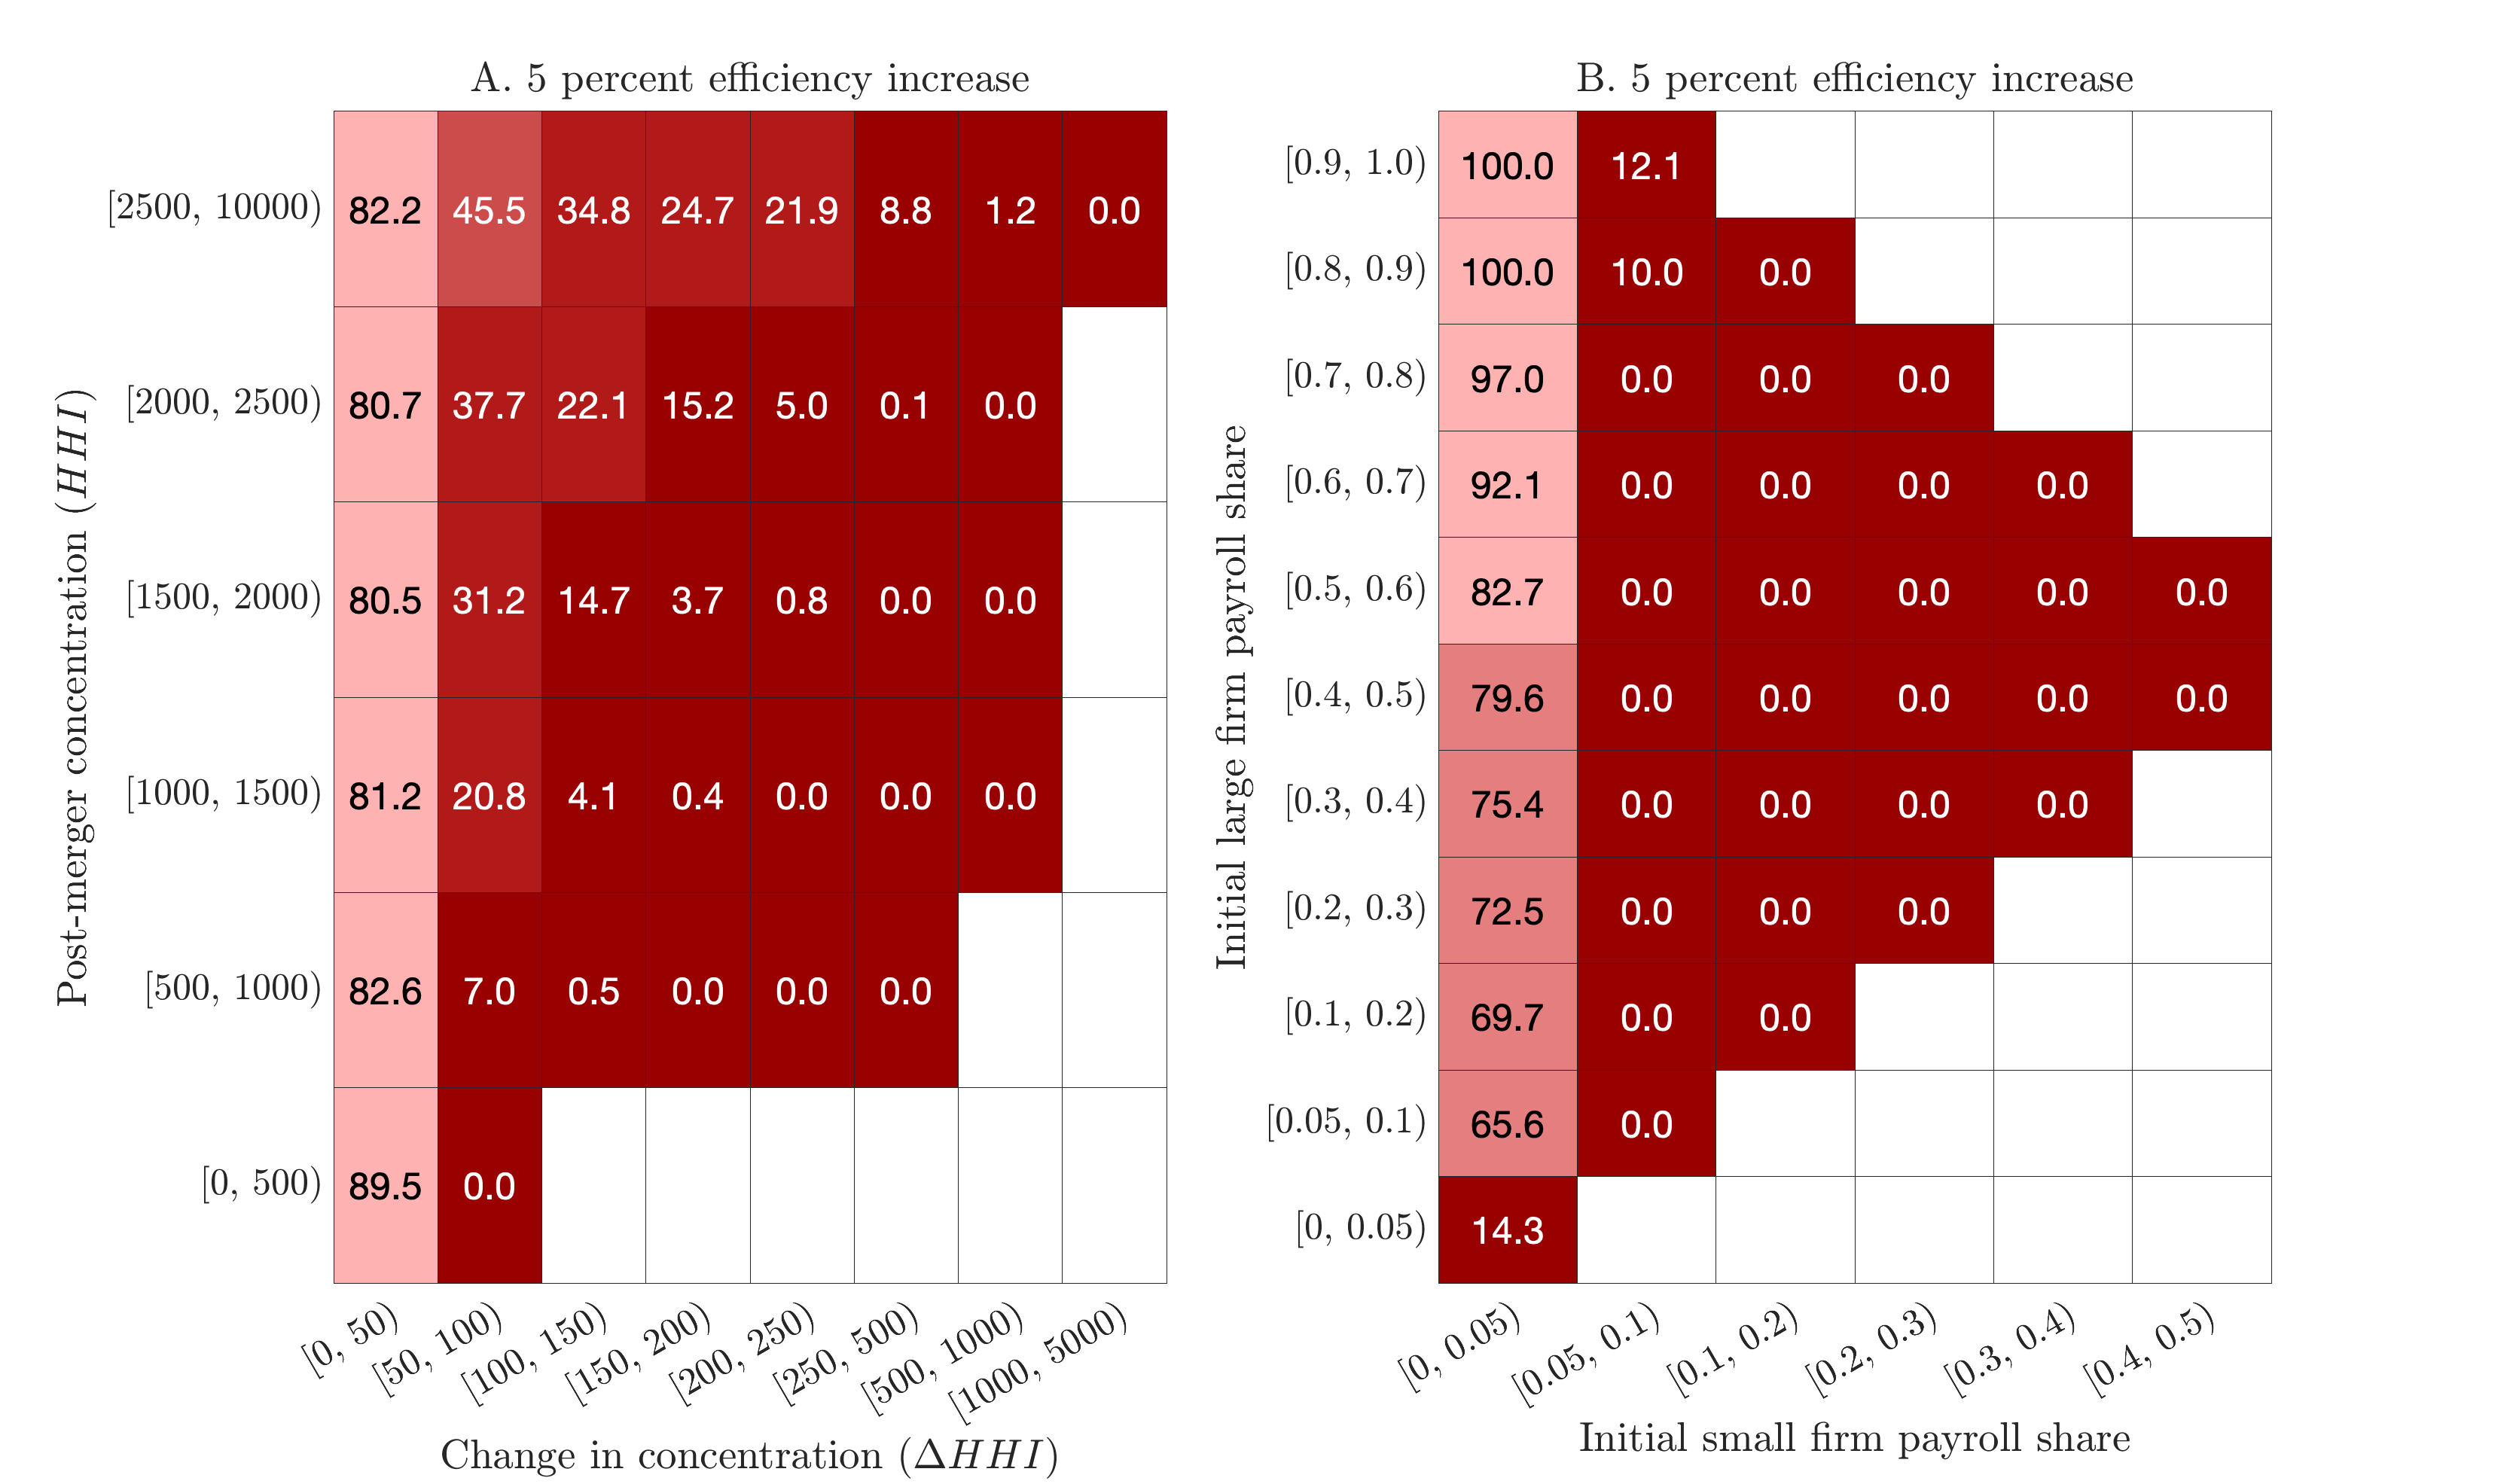
\includegraphics[width=18cm]{../results/figures/fig1_merger_simulation_heatmap}
	\caption{Fraction of mergers yielding worker surplus gain for 5 percent efficiency gain}
        \label{fig:hhi_cutoff_hm}
        \begin{footnotesize}
\begin{flushleft}
 \textit{Notes. Merger simulation designed to match representative set of firms based on \citet{Arnold}, see text for details. Post-merger $HHI$ (y-axis) and $\Delta HHI$ (x-axis) are computed naively using the combined pre-merger shares of the merging firms.  Panel A  reports the fraction of mergers that are worker surplus neutral  when the merger generates an efficiency gain of 5 percent at both plants, as defined by equation \eqref{eq:pi_delta_augmented}.  Panel B repeats the same exercise as Panel A, except Panel B stratifies by the merging firms' pre-merger local payroll market shares. The x-axis is the local payroll of the smaller of the two merging firms.  }   
 \end{flushleft}
\end{footnotesize}
\end{figure} 
 
For a given level of ``Type I'' error tolerance and a given level of assumed merger efficiency gains, regulators can use our figures to inform policy. 
Suppose a regulator is presented with a proposed merger with an initial small firm share of $4$ percent and a large firm share of $18$ percent. 
Figure \ref{fig:hhi_cutoff_hm}B says that under an assumed productivity gain of $5$ percent, there is a $69.7$ percent chance that the merger yields a worker surplus gain. 
First, depending on the amount of risk the regulator is prepared to accept, relative to this 69.7 percent chance of gain, the regulator can permit or block the merger. 
Second, depending on the assumed efficiency gain the regulator may also behave differently. 
Appendix Figure \ref{fig:shares_cutoff_hm2} shows that under an efficiency gain of 10 percent, the chance of gains increases to a $97.7$ percent.  
Hence, based on the regulator's tolerance for risk and priors on merger efficiency gains, regulators may use Appendix Figures \ref{fig:hhi_delta_hm} and \ref{fig:shares_delta_hm} to determine which mergers should be reviewed. 

\section{Downward wage pressure}\label{sec:dwp}

In the product market,   \textit{upwards price pressure} and \textit{gross upwards price pressure indexes} are commonly referenced metrics to evaluate the effects of mergers on consumers \citep[e.g.][]{farrell2010antitrust,naidu2018antitrust}. 
In this section, we mirror the product market approach. 
We define and then derive closed-form share-based formulas for \textit{downwards wage pressure} and \textit{gross downwards wage pressure}.
 
\paragraph{Downward wage pressure.} 
To derive the first of our formulas, we combine and rearrange the first order conditions of the merged firm's optimal employment choice at Plant 1 (equation \ref{eq:merger_foc}). 
This yields the following expression for wages (a symmetric equation exists for Plant 2):
{\vspace{-.2cm}\begin{align}
	\label{eq:diversion_dwp}
	w_{1j} & = \Bigg(\frac{\varepsilon_{1j}}{\varepsilon_{1j} + 1}\Bigg) \Bigg( z_{1j} - \underbrace{n_{2j} \frac{\partial w_{2j}}{\partial n_{1j}}}_{:=\text{Downward wage pressure}}\Bigg)
\vspace{-.2cm}\end{align}}

We formally define downward wage pressure to be the term $n_{2j} \frac{\partial w_{2j}}{\partial n_{1j}}$. 
This term is equivalent to a per-worker,  lump-sum \emph{labor cannibalization tax}.\footnote{
    To see this, consider a single plant that chooses $n_{1j}$ to maximize 
    $\pi_{1j} = z_{1j} n_{1j} - (w_{1j}+\overline{\tau})n_{1j}$,
    where $\overline{\tau}$ is a per-worker payroll tax. 
    When the first order condition is evaluated at $\overline{\tau}=n_{2j} \frac{\partial w_{2j}}{\partial n_{1j}}$, the equivalence of the first order conditions at Plant 1 follows immediately.} 
What generates this tax?
When the newly merged firm hires at Plant 1, it must pay higher wages at Plant 2 to keep employment constant at Plant 2. 
Since there are $n_{2j}$ workers employed at Plant 2, the total increase in costs for Plant 2 is $n_{2j} \frac{\partial w_{2j}}{\partial n_{1j}}$. 
Before the merger, this does not enter either firm's wage-setting decision. 
After the merger, the merged firm's objective is to maximize the combined profits of Plants 1 and 2, in which case it internalizes this effective tax, thus lowering the marginal benefit of hiring at both plants.

Using the labor supply system, we can express the Downward Wage Pressure term in \eqref{eq:diversion_dwp} as a share-based formula (a symmetric equation defines $DWP_{2j}$ at Plant 2):
\begin{align}\label{eq:dwp}
	\text{DWP}_{1j}:=n_{2j}\frac{\partial w_{2j}}{\partial n_{1j}}=w_{1j}\left(\frac{1}{\theta}-\frac{1}{\eta}\right)s_{2j}
\end{align}%
Thus downward wage pressure at Plant 1 is a simple function of Plant 2's payroll share of the local labor market, Plant 1's wage rate, and labor substitutability parameters  $\eta$ and $\theta$ (of which estimates are provided in Table \ref{tab:param_summary}). 
Intuitively, the larger the share of Plant 2 in the labor market, the greater the downward wage pressure. 
Likewise, the larger the degree of substitutability across plants within the market (i.e., higher $\eta$), the greater the downward wage pressure. 
High values of $\eta$ imply high degrees of head-to-head competition. 
When firms that engage in more head-to-head competition merge, small wage changes more aggressively reallocate employment, increasing this `tax'. 

\paragraph{Gross downward wage pressure.}  
The DWP defined in equation \eqref{eq:dwp} is in wage units, making its cardinal value difficult to interpret in practice. 
This leads  us to  define the gross downward wage pressure index. 
To derive the gross downward wage pressure index (GDWPI), we simply divide equation \eqref{eq:dwp} by $w_{1j}$:
\begin{align}\label{eq:gdwp}
	\text{GDWPI}_{1j}:=	\frac{\text{DWP}_{1j}}{w_{1j}} = \left(\frac{1}{\theta}-\frac{1}{\eta}\right)s_{2j}, \qquad \text{GDWPI}_{1j}\in \Big[0, \theta^{-1}-\eta^{-1}\Big]
\end{align}%
The GDWPI yields a particularly simple interpretation of downward wage pressure as a tax rate on the wages of workers at Plant 1.\footnote{
    To see this, consider a single plant that chooses $n_{1j}$ to maximize 
	$$z_{1j} n_{1j} - (w_{1j}+\overline{\tau})n_{1j}.$$
	Taking FOCs, we have $z_1-\overline{\tau}-w_1(\varepsilon^{-1}+1)=0$. 
    This can be rearranged to see $z_1-\overline{\tau}\frac{w_1}{w_1}-w_1(\varepsilon^{-1}+1)=z_1-w_1(\varepsilon^{-1}+1+\frac{\overline{\tau}}{w_1})=0$.
    Hence $\overline{\tau}/w_1$ has the interpretation of a tax on worker wages. Letting   $\overline{\tau}=n_{2j} \frac{\partial w_{2j}}{\partial n_{1j}}$ yields the GDWPI.}  
When Plant 1 hires, market wages increase, causing the labor costs at Plant 2 to increase. 
$\text{GDWPI}_{1j}$ summarizes this extra cost of wages at Plant 2  as a fraction of wages at Plant 1. 
Hence, we treat $\text{GDWPI}_{1j}$ as a wage tax and express it in percentage terms.
Given its sole dependence on the merging plants' local labor market shares, this formula can be readily applied to any industry with appropriate estimates of within- and across-market substitutability ($\eta$ and $\theta$). 
We view our economy-wide estimates of $\eta$ and $\theta$ as a good initial benchmark, while acknowledging that obtaining industry and geography specific estimates should be a priority of future work.\footnote{
    Recall from Table \ref{tab:param_summary}, $\theta=0.45$, and $\eta=10.85$, giving $\theta^{-1}-\eta^{-1}=2.29$.}

\begin{figure}[t!]
	\begin{center}
		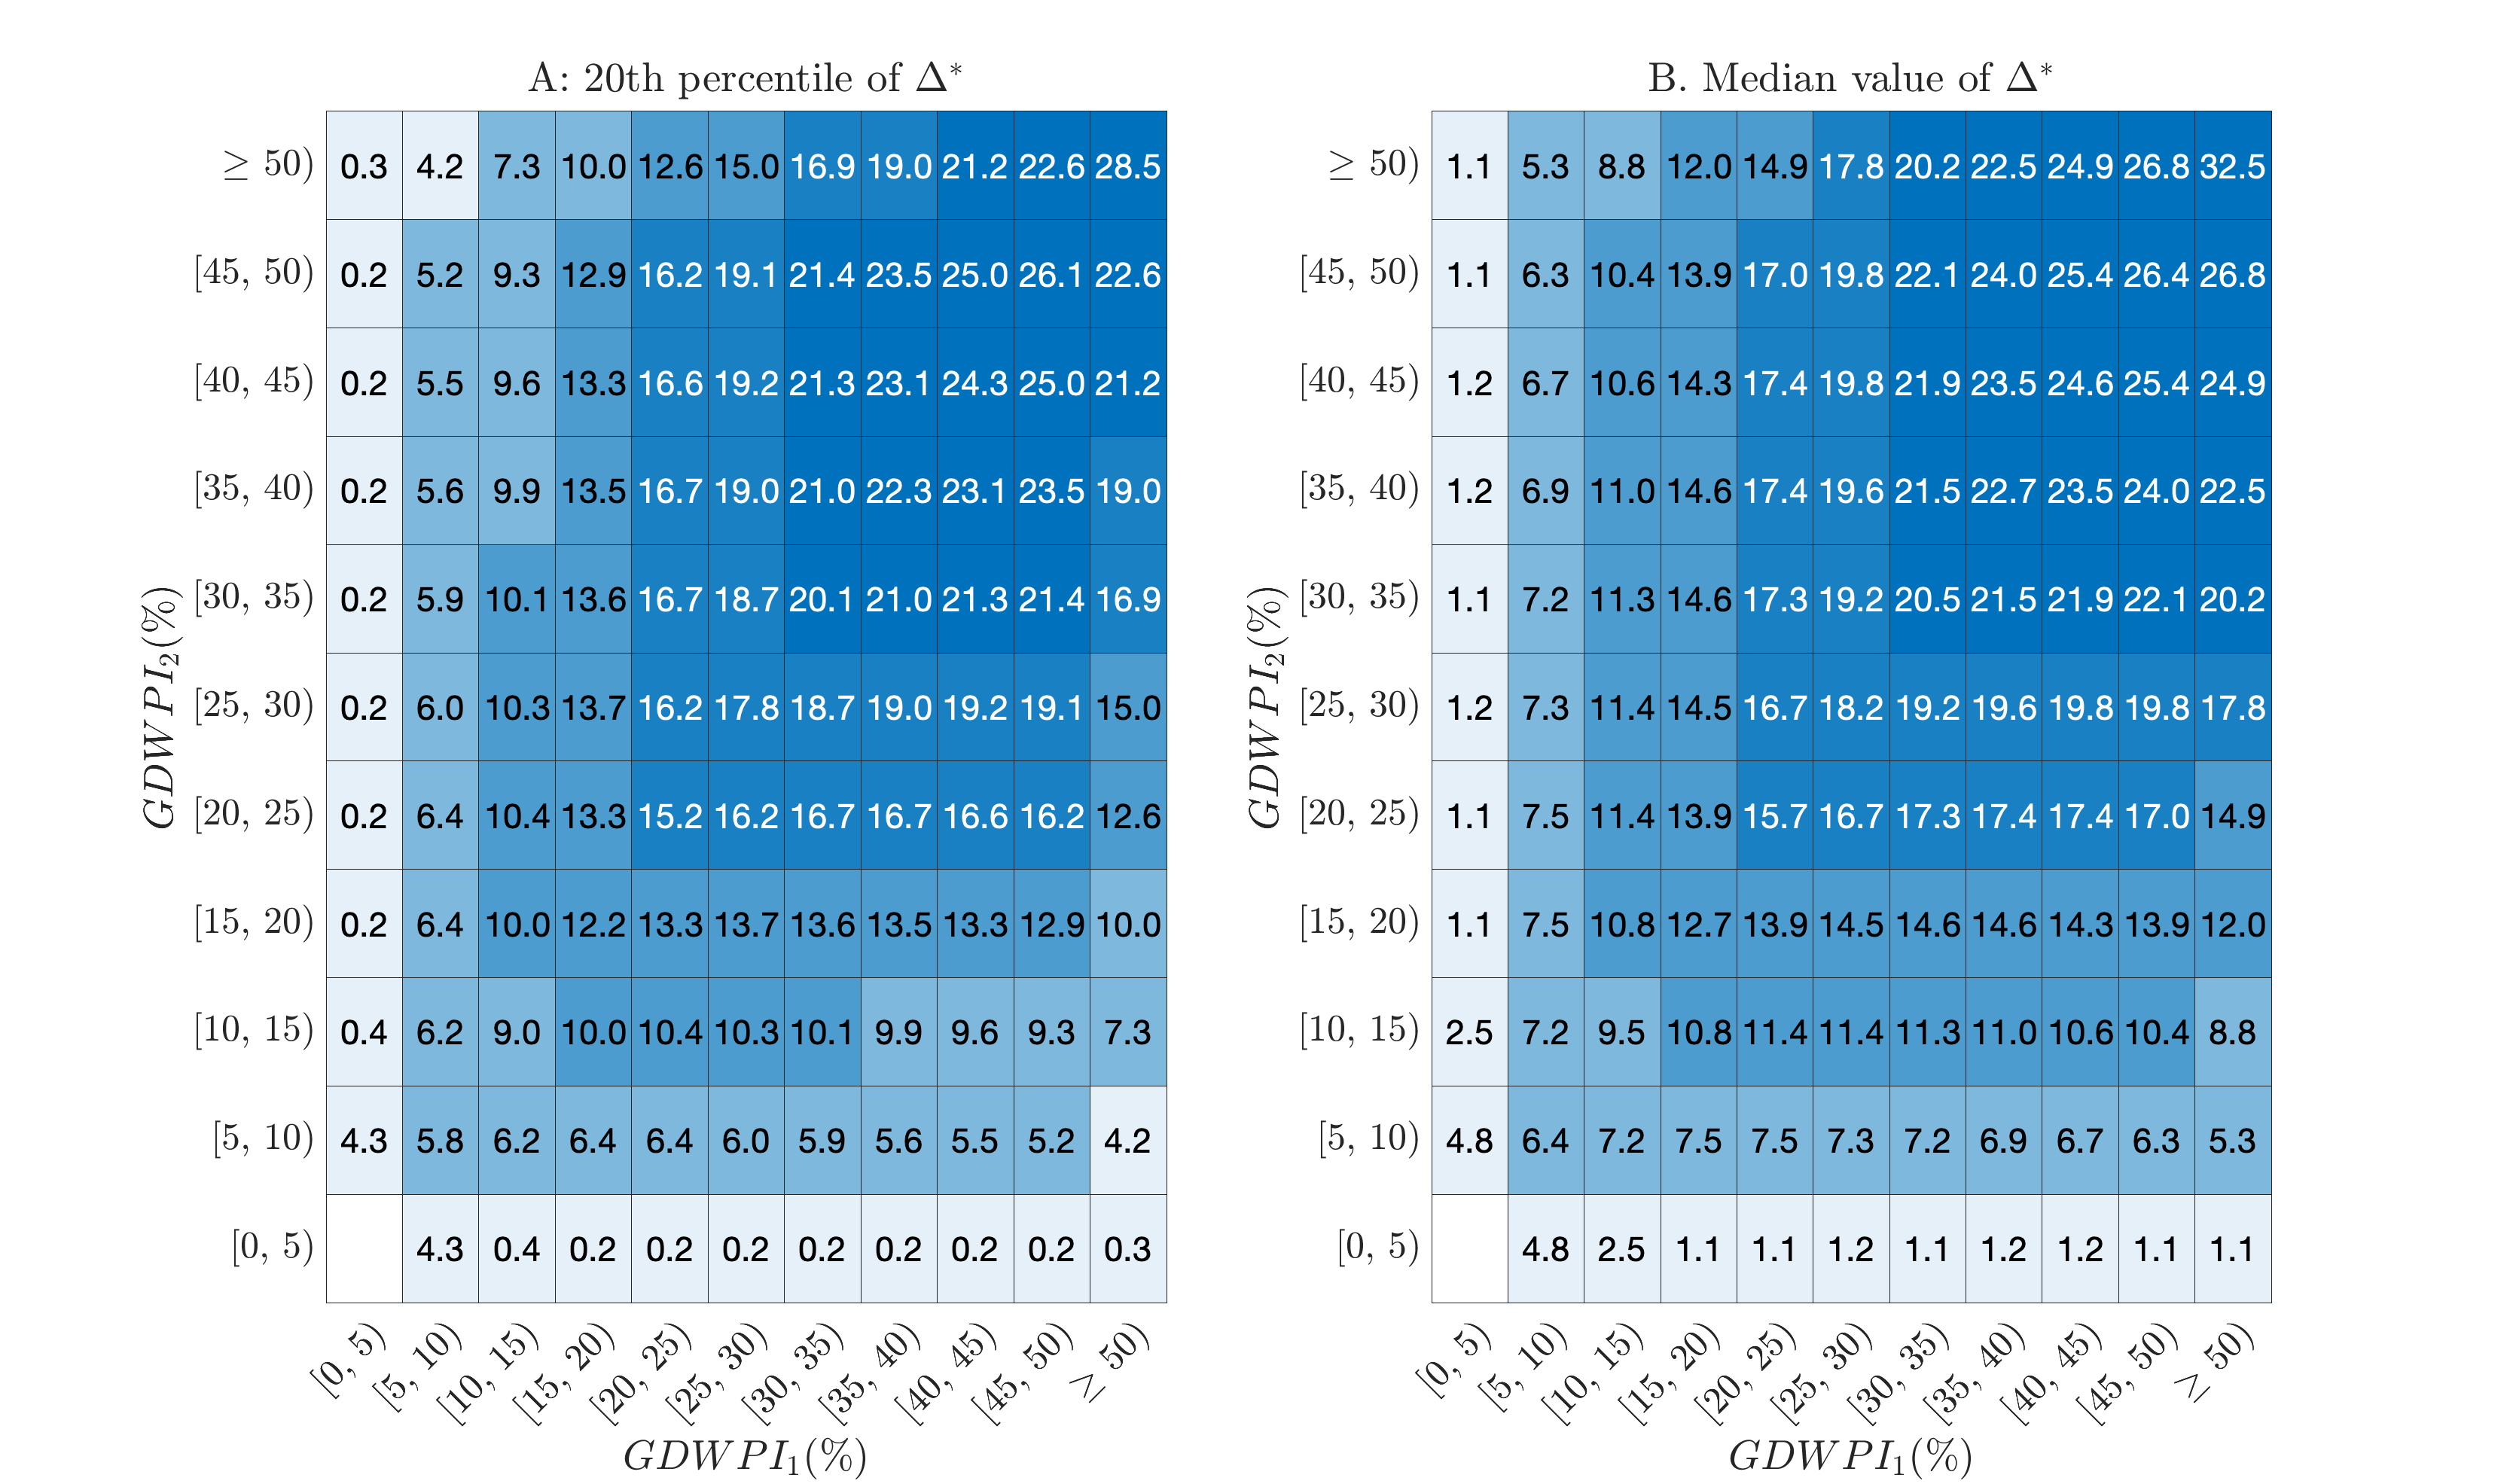
\includegraphics[width=19cm]{../results/figures/fig2_dwp_heatmap}
		\caption{Productivity gains necessary to yield worker surplus neutrality stratified by gross downward wage pressure at each of the merging plants. The gross downward wage pressure is defined by equation \eqref{eq:gdwp}, and multiplied by 100}\label{fig:gdwp}
		\vspace*{-.25cm}
	\end{center}
 \begin{flushleft}
 	\textit{Notes. Merger simulation designed to match representative set of firms based on \citet{Arnold}, see text for details. Post-merger $GDWPI_1$  (x-axis) is gross downward wage pressure at plant 1. Post-merger $GDWPI_2$  (y-axis) is gross downward wage pressure at plant 2.  Panel A reports the 20th percentile of required efficiency gains for worker surplus neutrality.   Panel B reports the 50th percentile (median) of required efficiency gains for worker surplus neutrality. }   
 \end{flushleft}
\end{figure}

 
Figure \ref{fig:gdwp} plots the required efficiency gains (REGs) for worker surplus neutrality ($\Delta^*$) as a function of both plants' gross downward wage pressure (defined by equation \ref{eq:gdwp}).  
Figure \ref{fig:gdwp} is constructed as follows:\vspace*{-.2cm}
{\small\begin{enumerate}
	\item For each of the $N=200,000$ simulated mergers Section \ref{sec:Guidelines}, we index the merger by $n\in\{1,\ldots,200,000\}$ and compute the gross downward wage pressure index (GDWPI) for each plant involved in the merger using equation \eqref{eq:gdwp}.\footnote{
            As in  Section \ref{sec:Guidelines}, we only  consummate the merger if $i$ and $i'$'s average pre-merger employment is greater than $\tilde{n}=46$ in order to match the observed median merger size in \citet{Arnold}'s representative sample of mergers in the U.S. }
 \vspace*{-.2cm}
	\item Additionally, for each merger,  compute the REG, $\Delta^*_n$, necessary for worker surplus neutrality and store these in a vector $\{\Delta_n^\ast\}$.\vspace*{-.2cm}
	\item Bin mergers based on the recorded GDWPI value at each plant. Without loss of generality, the $x$-axis is the GDWPI at Plant 1, the $y$-axis is the GDWPI at Plant 2.\vspace*{-.2cm}
	\item For all mergers that have a given GDWPI combination at Plant 1 ($x$-axis) and Plant 2 ($y$-axis), Figure \ref{fig:gdwp}A reports the 20th percentile of the  REG distribution, $\{\Delta_n^\ast\}$, while  Figure \ref{fig:gdwp}B reports the median of the  REG distribution.\vspace*{-.2cm}
\end{enumerate}}
%For example, the southwest-most cell of  Panels A and B isolate all mergers in which GDWPI at Plant 1 is less than 5 percent and GDWPI at Plant 2 is less than 5 percent. 

%Among all of those mergers, Panel A  of Figure \ref{fig:gdwp} reports the 20th percentile REG $\Delta_n^*$  and  Panel B  of Figure \ref{fig:gdwp} reports the median  $\Delta_n^*$. 
%The median REG is 0.13 in Panel B. 
%This implies that the majority of mergers with gross downwards wage pressure indexes less than 5 percent generate a worker surplus gain as long as merger efficiency gains are at least 0.13\%.
%\redSM{[This doesn't quite sound right / too aggressive. I think we want to say something like:
%\emph{When the GDWP for both firms is more than 5 percent, the REG thershold is at least 5 percent}.
%The issue is that we are merging all firms, so there are so many tiny mergers, so we don't want to focus on something like the median.} 

For example, consider the second diagonal element of Figure \ref{fig:gdwp}A, which corresponds to mergers in which the GDWPI lies between 5 percent and 10 percent at both plants. 
There are thousands of simulated mergers for which $\text{GDWPI}_{1j}\times100\in[5,10)$ and $\text{GDWPI}_{2j}\times100\in[5,10)$.
Among all those mergers, Panel A  of Figure \ref{fig:gdwp} reports the 20th percentile REG $\Delta^*$  and  Panel B  of Figure \ref{fig:gdwp} reports the median  $\Delta^*$. 
In Panel A, the 20th percentile REG among those mergers is 5.8 percent. 
This means that if regulators assumed that firms' productivity increased by 5.8 percent following a merger, worker surplus neutrality only occurs in 20 percent of consummated mergers in which both firms' GDWPI is between 5 and 10 percent.  
Panel B shows that the \textit{median} $\Delta_n^*$ among those mergers is 6.4 percent. 
If regulators assumed that firms' productivity increased by 6.4 percent following a merger, 50 percent of mergers in which firms' GDWPI is between 5 and 10 percent yield worker surplus neutrality and leave workers unharmed.  
 
Consider mergers in which the GDWPI is more than 10 percent at both plants. 
Among all mergers in the upper quadrant of Panel A  of Figure \ref{fig:gdwp}, the 20th percentile of  $\Delta^*$ is bound below by 7.30 percent.
In other words, if we take mergers that induce gross downward wage pressure of 10 percent or more at both plants, more than 80 percent of these mergers would generate a welfare loss under an assumed efficiency gain of 5 percent.
 
\subsection{Aggregate effects of mergers}

Under our assumption of ex-ante identical markets, mergers will occur in all markets in the long-run. Therefore, we treat the aggregate effects of \textit{allowed mergers} on output and labor's share of income as the \textit{long-run economy-wide effects}. Table \ref{tab:agg_effects} reports our results. In Panel I, we compute total output in affected markets pre-merger and compare that to total output post-merger.  We find that in the absence of efficiency gains from mergers, output falls for both sets of guidelines. For efficiency gains greater than 1\%, output increases after the merger for both sets of guidelines. Beyond efficiency gains of 5\%, output gains are greater for looser guidelines. Panel II repeats this exercise for labor's share of income. Across all potential efficiency gains, labor's share of income falls. The decline in labor's share of income is greatest when productivity gains are larger. This is because firms with large productivity gains experience the greatest increase in labor market power. They produce more, and they pay workers more, but their markdowns widen, lowering workers' share of the ``economic pie.'' For any level of efficiency gains, the downward pressure from mergers on labor's share of income is mitigated by stricter guidelines. Panel III shows the opposite pattern for the share of profit income, implying that the decline in the labor share is offset by an increase in the profit share, while the capital share remains largely unchanged.
	
Figure \ref{fig:agg_graph}	plots the aggregate output, payroll, and profit effects of mergers in affected markets. We see that efficiency gains must exceed $\approx$4.5\% before worker payroll increases (consistent with our earlier worker surplus analysis). However, output gains are always positive when efficiency gains exceed $\approx$1\%. Thus, there is a range of mergers (with efficiency gains between $\approx$1\% and $\approx$4.5\%) that hurt workers but generate output gains. This exercise highlights the tradeoffs inherent in the adoption of a worker surplus metric: stricter guidelines prevent worker harm at the expense of lost output.
 
 \begin{table}[p!]
    \centering
    %\resizebox{\textwidth}{!}

    \begin{tabular}{l @{\hspace{2em}} c @{\hspace{1.5em}}c}
\toprule
 & \multicolumn{1}{l}{\textbf{{------1982/2023 guidelines------ $\quad$ }}} & \multicolumn{1}{l}{\textbf{{------2010 guidelines------}}} \\ 
DOJ/FTC Market Classification & \textit{Highly Concentrated} & \textit{Highly Concentrated} \\ 
Threshold (HHI, $\Delta$HHI) & (1800, 100) & (2500, 200) \\ 
 & (1) & (2) \\ 
\midrule
\multicolumn{3}{l}{\textbf{I. Percentage Change in Output Relative to No-Merger Baseline}} \\ 
0 Percent Efficiency Gain & -0.16 & -0.24 \\ 
1 Percent Efficiency Gain & 0.03 & -0.03 \\ 
2 Percent Efficiency Gain & 0.23 & 0.19 \\ 
3 Percent Efficiency Gain & 0.44 & 0.42 \\ 
4 Percent Efficiency Gain & 0.65 & 0.65 \\ 
5 Percent Efficiency Gain & 0.87 & 0.89 \\ 
\midrule
\multicolumn{3}{l}{\textbf{II. Change in Labor Share Relative to No-Merger Baseline}} \\ 
0 Percent Efficiency Gain & -0.29 & -0.40 \\ 
1 Percent Efficiency Gain & -0.31 & -0.43 \\ 
2 Percent Efficiency Gain & -0.34 & -0.46 \\ 
3 Percent Efficiency Gain & -0.37 & -0.50 \\ 
4 Percent Efficiency Gain & -0.40 & -0.53 \\ 
5 Percent Efficiency Gain & -0.44 & -0.57 \\ 
\midrule
\multicolumn{3}{l}{\textbf{III. Change in Profit Share Relative to No-Merger Baseline}} \\ 
0 Percent Efficiency Gain & 0.29 & 0.40 \\ 
1 Percent Efficiency Gain & 0.31 & 0.43 \\ 
2 Percent Efficiency Gain & 0.34 & 0.46 \\ 
3 Percent Efficiency Gain & 0.37 & 0.50 \\ 
4 Percent Efficiency Gain & 0.40 & 0.53 \\ 
5 Percent Efficiency Gain & 0.44 & 0.57 \\ 
\bottomrule 
\end{tabular} 
    \caption{Aggregate effects of applying the 1982/2023 and 2010 guidelines. \label{tab:agg_effects}}
    \begin{footnotesize}
        \begin{flushleft}
            \textit{Notes. Merger simulation designed to match representative set of merging firms based on \citet{Arnold} (see text for details). Column (1) applies the 1982/2023 guidelines.  In Column (1), all mergers with post-merger concentration/change in concentration above ($HHI=1800, \Delta HHI=100$) are blocked. Column (2)  applies 2010 guidelines.   In Column (2), all mergers with post-merger concentration/change in concentration above ($HHI=2500, \Delta HHI=200$) are blocked. Panel I  reports the change in aggregate output pre-merger relative to post-merger  when the merger generates an efficiency gain of $\{0\%, 1\%,2\%,3\%,4\%,5\%\}$  at both plants, as defined by equation \eqref{eq:pi_delta_augmented}. Panel II repeats this exercise for labor's share of income. Panel III repeats this exercise for the profit share.  }   
        \end{flushleft}
    \end{footnotesize}
\end{table}
 
\begin{figure}[t!]
    \begin{center}
        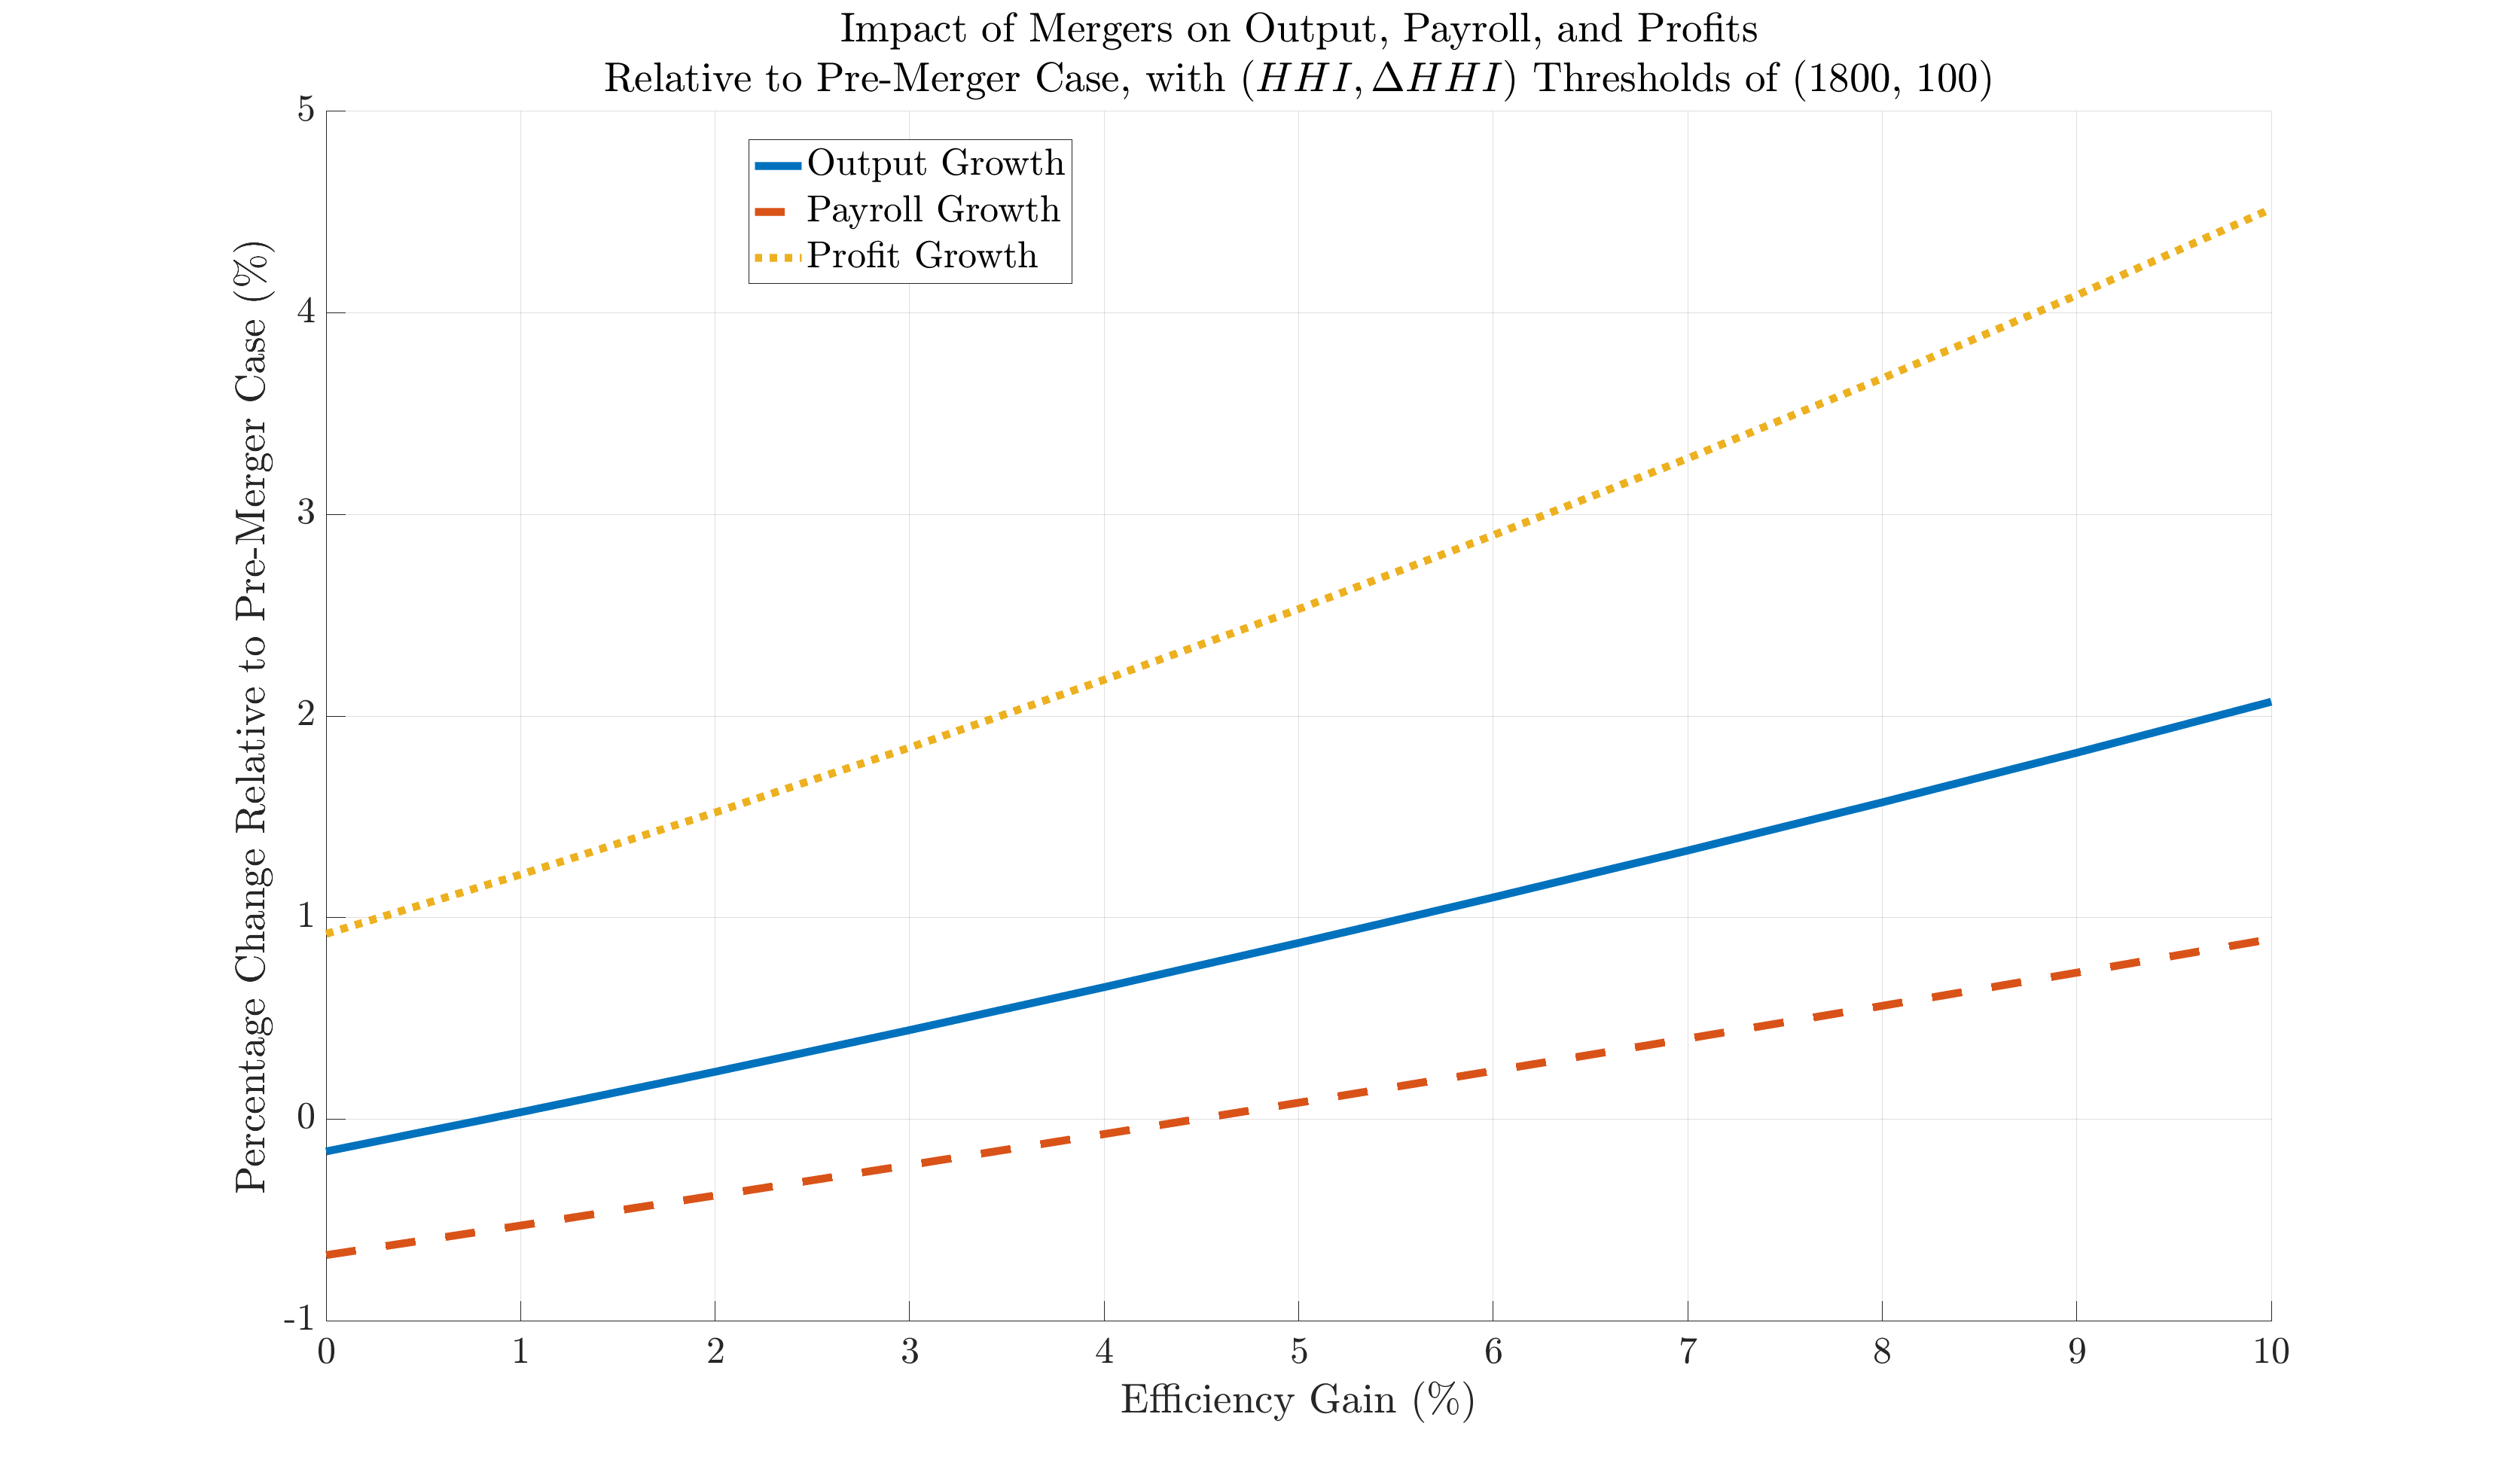
\includegraphics[width=18cm]{../results/figures/fig3_aggregates}
        \caption{Aggregate effects of mergers on output, payroll, and profits under 1982/2023 guidelines. }\label{fig:agg_graph}
        \vspace*{-.25cm}
    \end{center}
    \begin{flushleft}
        \textit{Notes. Merger simulation designed to match representative set of firms based on \citet{Arnold}, see text for details. The x-axis is the assumed efficiency gains from merger   at both plants, as defined by equation \eqref{eq:pi_delta_augmented}. The y-axis plots the aggregate output/payroll/profit gains among affected markets relative to the pre-merger economy. }   
    \end{flushleft}
\end{figure}
 
\section{Robustness and Caveats}
\label{sec:robust}

\paragraph{Labor redundancy.} 
Our benchmark model assumes that there are decreasing returns to scale, implying no scope for labor redundancy.
To introduce a labor redundancy channel,  we allow for increasing returns to scale production functions in Section \ref{app:irs}.
We borrow estimates from the spatial literature (\citet{ciccone1993productivity}, \citet{davis2014macroeconomic}, and \citet{herkenhoff2018tarnishing} among others) and assume an increasing returns parameter of 3\%, i.e. $\alpha=1.03$.  
With increasing returns, pre-merger production can be achieved at a single consolidated plant using fewer workers than previously employed pre-merger, yielding endogenous efficiency gains from merging. 
In other words, some of the initial labor used to produce would become redundant if the plants were to merge and maintain identical output. 
This exercise also approximates the effects of explicitly modeling fixed costs of labor (i.e. each company needs one accountant, regardless of the number of plants operated), which gives rise to a similar notion of increasing returns and labor redundancy. 
Accounting for labor redundancy reduces the required efficiency gains for worker surplus neutrality. 
The REG for permitted mergers under the 1982/2023 guidelines falls from 4.68\% (Table 3) to 1.80\%.
The REG for permitted mergers under the 2010 guidelines falls from 5.96\% (Table 3) to 2.85\%. 
Hence, in both cases worker surplus gains are achieved at much lower assumed levels of efficiency gains, in particular at levels less than the standard 5\% assumption. 

\paragraph{Market structure.} 
Our model assumes that differences in productivities and numbers of firms are the only traits that differentiate markets. 
Markdowns differ because the market shares of firms differ, but the underlying parameters governing markdowns ($\eta,\theta$) are common across markets. 
There are a number of reasons to believe markets differ beyond these attributes.
In Appendix \ref{app:eta_theta_robust}, we  recompute our main quantitative exercises under the assumption that $\eta$ and $\theta$ are 10\% higher or lower than our estimated values. 
In all cases, the 2010 guidelines yield permitted mergers with an average REG above 5\%. 
With one exception, the 1982/2023 guidelines yield permitted mergers with an average REG less than 5\%.
The only exception is the case where only $\theta$ is reduced by 10\%, which delivers much more market power to the largest firms. 

Another concern is that more data-driven methods of classifying markets would yield different results. 
Our paper defines markets as NAICS 3-digit industries within a commuting zone. We assume workers are free to move across markets. 
This market definition only determines the boundary of firm wage competition. 
In island models such as \citet{berger2023anatomy}, \citet{bagga2023firm}, and \citet{jarosch2024granular} workers are fixed in a single market, and so the market definition determines \textit{both} worker mobility and the boundary of firm wage competition. 
These authors attempt to cluster workers into markets so as to minimize leakage rates in one way or another. 
In the case of Norway, \citet{berger2023anatomy} compare leakage rates across market definitions and find that industry, occupation and flow based methods perform similarly (all leakage rates based on industry, occupation, or flow clustering range from 50\% to 70\%). 
Despite different economic settings, \citet{berger2023anatomy} also estimate a similar degree of monopsony power and markdowns using occupation based clustering methods to the current paper. 
Since comparable data does not exist for the United States, we cannot determine how alternate market definitions would alter our results. 
 
\paragraph{Wage discrimination.} Models based on \citet{Robinson1933}, such as ours, typically assume that workers are homogeneous and paid a common wage. Several quantitative papers have relaxed the worker homogeneity assumption.  Recently, \citet{deb2022drives}  extended \citet{berger2022labor} to include multiple worker types. They estimate the model using matched employer-employee data in the U.S. and find evidence in support of oligopsony. They estimate markdowns in the range of 30\% to 40\%, similar to the current paper. Others have modeled worker-firm specific contracts in search and matching settings (e.g. \citet{bagga2023firm}, \citet{berger2023anatomy} and \citet{jungerman2023dynamic}). Unlike the firm-level data employed in this paper, these frameworks typically require matched employer-employee data in order to be estimated, and these frameworks have not yet been integrated with theories of multi-plant ownership. We believe such extensions will yield important insights; however, they lie beyond the scope of the current paper.
 

\paragraph{Product market power.}  
When assessing the merger guidelines, our approach was to keep product market power fixed. 
Through the lens of the merger guidelines, this is the correct counterfactual to assess worker welfare and worker harm. The 2023 merger guidelines make this explicit: 
\emph{``If the merger may substantially lessen competition or tend to create a monopoly in upstream
		markets, that loss of competition is not offset by purported benefits in a separate downstream product
		market.''}
In other settings, researchers may want to understand the interaction between product and labor market power. 
To facilitate those discussions, we demonstrate how our  framework can be modified to incorporate monopolistic pricing  in Appendix \ref{app:product_market}.
Recent work by \citet{deb2022drives} incorporates an even richer theory of variable product markups into  \citet{berger2022labor}.

\paragraph{Employee market power.}   In our theory, employees are atomistic and have no market power. 
While the share of unions is small and declining in the U.S., roughly 6\% of private sector workers remain unionized in 2024.\footnote{\url{https://www.bls.gov/news.release/pdf/union2.pdf} }
	Recent work by \citet{azkarate2020aggregate} develops a theory in which unions interact with strategic oligopsonists. 
They model unions using Nash bargaining between the firm and the collective set of employees. 
Models of search and matching also give rise to a notion of hold-up power among employees (e.g. \citet{bagga2023firm} and \citet{berger2023anatomy}).
Either of these approaches (unions and search) can, in theory, be integrated into a model of multi-plant ownership.
However, a number of assumptions regarding the post-merger union structure and the  post-merger search technologies at the combined plants must be made and justified.  
We leave such an endeavor to future work. 
 
\paragraph{Alternate thresholds, employment, and output.} 
Lastly, the Appendix to this paper provides a number of more detailed tables and merger thresholds based on alternative efficiency gains.
Appendix \ref{app:uni} provides uni-dimensional merger guidelines based on $HHI$s alone or $\Delta HHI$'s alone. 
Appendix \ref{app:output} analyzes the output response to mergers. 
Appendix \ref{app:emp} analyzes the employment response to mergers. 
Finally, in Appendix \ref{app:error}, we provide Type I and Type II error rates for the 1982/2023 and 2010 merger guidelines.
 

\section{Conclusion}
 
This paper provides a quantitative framework of multi-plant ownership and monopsony. 
We use the framework to theoretically characterize the effects of mergers on employment, wages, and worker welfare. 
We calibrate our model economy to the United States and show that the model generates empirical patterns consistent with recent causal analysis of the labor market effects of mergers \citep{Arnold}, including how post-merger employment and wage losses vary by observable characteristics like concentration. Having validated our model, we then simulate a representative set of mergers in the United States and conduct a variety of merger review exercises. 

Our main exercise compares the 1982/2023 and 2010 product market merger review guidelines when applied to the labor market. 
Under a standard assumed efficiency gain of 5 percent, our framework suggests that more stringent 1982/2023 guidelines in the labor market are required for worker surplus neutrality.
If the DOJ and FTC are sufficiently concerned with conserving resources by reviewing only those mergers most likely to harm workers while ensuring that workers are unharmed by permitted mergers, then the 1982/2023 guidelines in which mergers are presumed anticompetitive whenever post-merger concentration exceeds $(HHI=1800, \Delta HHI=100)$ achieve that goal. 
On the other hand, the 2010 guidelines in which mergers are presumed anticompetitive whenever post-merger concentration exceeds  $(HHI=2500, \Delta HHI=200)$ do not achieve that goal.  
Moreover, if efficiency gains are less than 5\%---as argued by recent empirical studies---then labor markets would require guidelines tighter than the 1982/2023 guidelines. 
%As this paper was being written and revised, the 2023 Merger Guidelines ultimately adopted the 1982 thresholds for the labor markets. 

Our paper stops short of computing the optimal policy -- such an exercise requires information not available publicly, including merger review costs, and it also requires a stance on the ``objective function'' of the agencies as a whole. 
However, the results we present in this paper allow researchers and regulators to compare the probability of a merger generating a worker surplus loss under the different cut-offs for merger review that constitute current policy:
local payroll Herfindahls, merger-induced Herfindahl changes, and downward wage pressure.  
For a given level of ``Type I'' error tolerance---i.e. reviewing mergers that would increase worker surplus---our results allow a regulator to  formulate a locus of cut-offs for merger efficiency gains and concentration statistics.
For example, a less risk-averse or resource-poor regulator would only want to review a small number of mergers. 
Given an assumed efficiency gain, that regulator may use our tables and figures to choose a concentration threshold for merger review above which they expect only 20 percent of mergers to yield worker surplus gains. 
A more risk-averse or resource-rich regulator would want to review many mergers, hence setting lower concentration cut-offs for merger review.  
Our framework can be used to aid the determination of such thresholds in future work. 

 
Our paper provides several avenues for future work.  
First,  estimates of between-firm and between-market elasticities of substitution, $\eta$ and $\theta$, by industry or geographic market are an important input for future analysis. 
Second, several key theoretical predictions of the model---in particular, equalization of markdowns across merged firms---can be tested using estimates of firms' markdowns (for which one could follow the approach in 
\citet{yeh2022monopsony}). 
Third, directed mergers may give rise to moral hazard (changes in proposed mergers due to policy) that alter the tradeoffs outlined above. 
Important recent work attempts to model   directed mergers in product markets \citep{ThomasJMP,FilipJMP}. 
Similarly, we abstract from mergers across markets. 
Finally, we parallel the traditional practice of applying the consumer welfare standard when evaluating mergers. 
This traditional approach abstracts from questions of the effects of mergers on the level and distribution of profits, and instead focuses on consumers, or in our case, workers. 
Alternative views suggest higher profits should be given a positive weight. 
%We leave assessment of welfare under alternative approaches to future work. 

%We believe a number of avenues for future research exist. How are gains and losses from mergers distrbuted across households? How do non-wage aspects of jobs change? And is there a realiable empirical metho

%Why are tighter merger guidelines necessary in the labor market versus the product market? Our estimated across-market labor substitutability is lower than what is typically estimated in product markets. This implies greater scope for anticompetitive effects and therefore more stringent labor market merger review thresholds are required for workers to be just as well off after the merger.

%The tables in this paper and associated appendices can be combined with regulators' priors on efficiency gains to form optimal policy prescriptions. For a given level of ``Type I'' error tolerance and merger efficiency gain, regulators can use our figures to compute what fraction of mergers would yield worker surplus losses or gross downward wage pressure. 
%Based on the regulator's tolerance for risk and priors on merger efficiency gains, the results provided in this paper can inform regulators as to which mergers should be reviewed based on thresholds for observable local labor market Herfindahls, changes in local labor market Herfindahl mergers, and the degree of gross downward wages pressure induced by the merger.
%
% Lastly, the framework for merger analysis developed in this paper can also be used in other areas of antitrust law where defendants are accused of imposing restraints on labor markets. Section 1 of the Sherman Act prohibits anticompetitive restraints of trade like wage-fixing and market division. In recent years, section 1 lawsuits have been brought against numerous firms that have entered no-poach and wage-fixing agreements, including major franchises like McDonald’s, poultry processing firms like Perdue, and sports leagues like the NCAA. Cases have also been brought under section 2 of the Sherman Act against firms that engage in ``monopolization'' (or, here, monopsonization). For example, a Saudi-backed golf tour called LIV sued the PGA Tour for preventing its members from participating in LIV’s tournaments  (see \citet{posner2023new} for a survey of the cases). In both section 1 and section 2 cases, plaintiffs must usually establish that defendants have market power within a clearly defined market, and prove that the restraint or conduct in question reduces worker compensation. The methods used in this paper can be further developed to improve analysis in both instances.

%Lastly, we  provide guidance for using the Gross Downward Wage Pressure method for evaluating the impact of mergers on labor markets.

%Our finding support the extension of existing product market guidelines to labor markets may be rationalized under various regulator objectives. 

%Our main contribution is to estimate what we call the \emph{required efficiency gains} (REGs) necessary for a merger to make workers at least as well off as they were before the merger (worker surplus neutral) and to characterize how REGs vary with local labor market statistics (Herfindahls) and properties of the merging firms (their combined share of the market pre-merger).
%We view the REG as a useful benchmark as it provides a standard for merging firms to meet in terms of explaining the productivity benefits of the merger.
%It does not rely on measures of concentration, nonetheless we can link measures of concentration---used in current merger guidelines---to provide guidelines for policy. 

%We find that, under an assumed merger efficiency gain of 2 percent, more than 80 percent of mergers with a (naive) predicted concentration increase of $\Delta HHI_j$ of more than $100$ would in fact generate a worker surplus loss.  
%That is, a higher REG than 2 percent in needed to avoid worker surplus losses for the vast majority of mergers in which $\Delta HHI_j$ is greater than $100$. 
%This potentially rationalizes an extension of existing product market merger review guidelines for labor markets. 

%%%%%%%%%%%%%%%%%%%%%%%
%%BIBLIO
%%%%%%%%%%%%%%%%%%%%%%%
\clearpage \newpage
\begin{small}
	\bibliographystyle{econometrica}
	\bibliography{bib_12_14_22}
\end{small}

%%%%%%%%%%%%%%%%%%%%%%%
%% PUBLICATION APPENDIX
%%%%%%%%%%%%%%%%%%%%%%%
\newpage\clearpage
\setcounter{page}{1}

\appendix

\begin{center}
	\textsc{{\Large {Online Appendix}}}
\end{center}
\vspace*{.5cm}


\section{Proof - Proposition 3.1}
%\setcounter{section}{0}\renewcommand{\thesection}{A} \setcounter{equation}{0}
%\setcounter{table}{0} \setcounter{figure}{0} \renewcommand{\theequation}{A\arabic{equation}}
%\renewcommand{\thetable}{A\arabic{table}} %
%\renewcommand{\thefigure}{A\arabic{figure}}
%\renewcommand{\thesubsection}{\thesection.\arabic{subsection}}
\label{app:Math_merger}

\begin{itemize}
	\item In this section we prove the claims in Proposition 3.1. These are
	listed in a different order in Proposition 3.1, but here listed in
	the order that they are proved:
	\begin{enumerate}
		\item Following a merger, the markdowns at the merged firms are equalized
		and depend on the total market share, $\mu_{1j}=\mu_{2j}=\mu\left(s_{1j}+s_{2j}\right)$.
		\item Under either monopsony limit a merger has no effect on any labor market
		variables.
		\item The individual shares $s_{ij}$ of all non-merging firms increase.
		Therefore the total market share of merging firms falls.
		\item The wage index of non-merging firms \uline{decreases} and employment
		index \uline{increases}.
		\item Market wage $\mathbf{W}_{j}$ and employment $\mathbf{N}_{j}$
		decline, so total market pay $\mathbf{W}_{j}\mathbf{N}_{j}=\sum_{i\in j}w_{ij}n_{ij}$
		declines.
		\item The wages of both merging firms $w_{1j}$ and $w_{2j}$ decline. The
		wage index of merging firms \uline{decreases} and employment index
		\uline{decreases}.
	\end{enumerate}
	\item Parts 1 and 2 we prove under decreasing returns to scale. The remainder
	we establish under constant returns to scale. The proof of Part 3
	is the most involved, and remaining parts follow from Part 3 in a
	straight-forward manner.
\end{itemize}

\bigskip


\paragraph{\underline{Proposition 3.1, Part 1}: Common markdown.}
\begin{itemize}
	\item Throughout we assume $M_{j}\geq3$, and assign $i=1$ and $i^{\prime}=2$
	to the two merging firms.
	\item A merged firm chooses employment at both firms to maximize profits,
	where without loss of generality for this proof we can consider the
	case of a production function $f$$\left(\cdot\right)$ that already
	incorporates the (competitive) intermediate and capital choices
	\[
	\max_{n_{1j},n_{2j}}\:\left[f\left(z_{1j},n_{1j}\right)-w\left(n_{1j},\mathbf{N}_{-1j}\right)n_{1j}\right]+\left[f\left(z_{2j},n_{2j}\right)-w\left(n_{2j},\mathbf{N}_{-2j}\right)n_{2j}\right]
	\]
	\item When taking the first order condition, the firm understands that $n_{2j}$
	appears in $\mathbf{N}_{-1j}$ and vice versa.
	\item The first order condition for $n_{1j}$ is as follows, where we use
	$mrpl_{1j}=f_{n}\left(z_{1j},n_{1j}\right)$ to denote the marginal
	revenue product of labor
	\[
	\left(mrpl_{1j}-\frac{\partial w_{2j}}{\partial n_{1j}}n_{2j}\right)=\frac{\partial w_{1j}}{\partial n_{1j}}n_{1j}+w_{1j}
	\]
	\item Written this way we can see that in understanding that increasing
	$n_{1j}$ increases the wage at Firm 2, maps into an effective reduction
	in productivity at Firm 1.
	\item Recall that
	\begin{align*}
		w_{1j} & =n_{1j}^{\frac{1}{\eta}}\mathbf{N}_{j}^{\frac{1}{\theta}-\frac{1}{\eta}}\boldsymbol{X}\\
		w_{2j} & =n_{2j}^{\frac{1}{\eta}}\mathbf{N}_{j}^{\frac{1}{\theta}-\frac{1}{\eta}}\boldsymbol{X}
	\end{align*}
	\item Using this expression
	\begin{align*}
		mrpl_{1j}-w_{1j} & =\left(\frac{1}{\eta}+\left(\frac{1}{\theta}-\frac{1}{\eta}\right)s_{1j}\right)w_{1j}+\left(\frac{1}{\theta}-\frac{1}{\eta}\right)s_{1j}\frac{w_{2j}n_{2j}}{n_{1j}}\\
		mrpl_{1j}-w_{1j} & =\left(\frac{1}{\eta}+\left(\frac{1}{\theta}-\frac{1}{\eta}\right)s_{1j}\right)w_{1j}+\left(\frac{1}{\theta}-\frac{1}{\eta}\right)s_{2j}w_{1j}\\
		mrpl_{1j}-w_{1j} & =\left[\frac{1}{\eta}+\left(\frac{1}{\theta}-\frac{1}{\eta}\right)\left(s_{1j}+s_{2j}\right)\right]w_{1j}
	\end{align*}
	\item Therefore $w_{1j}=\mu\left(s_{1j}+s_{2j}\right)mrpl_{1j}$. Note that
	the same algebra can be applied to Firm 2. Therefore this establishes
	the first result:
	\[
	\mu_{1j}^{\prime}=\mu_{2j}^{\prime}=\mu\left(s_{1j}^{\prime}+s_{2j}^{\prime}\right)
	\]
	\item Note that the above algebra generalizes in a straight-forward way
	to the case of an arbitrary set of firms merging. Let the set of merging
	firms be $A$, then
	\[
	\mu_{ij}^{\prime}=\mu\left(\boldsymbol{s}_{jA}^{\prime}\right)\quad\boldsymbol{s}_{jA}^{\prime}=\sum_{i\in A}s_{ij}^{\prime}.
	\]
\end{itemize}
 \begin{flushright}
      $\square$
 \end{flushright}

\bigskip

\paragraph{\underline{Proposition 3.1, Part 2}: No effect of mergers in monopsony }
\begin{itemize}
	\item Consider the above problem of the merged firm in a monopsonistically
	competitive labor market
	\[
	\max_{n_{1j},n_{2j}}\:\left[f\left(z_{1j},n_{1j}\right)-w\left(n_{1j}\right)n_{1j}\right]+\left[f\left(z_{2j},n_{2j}\right)-w\left(n_{2j}\right)n_{2j}\right]
	\]
	\item Here the wage depends on $\mathbf{N}_{j}$ but since the firm
	is infinitesimal, it does not internalize its effect on $\mathbf{N}_{j}$.
	\item The first order condition for Firm 1 employment is:
	\[
	mrpl_{1j}=w^{\prime}\left(n_{1j}\right)n_{1j}+n_{1j}
	\]
	\item This is identical to the first order condition of Firm 1 in the pre-merger
	economy. Therefore there is no effect at all on employment and wages.
\end{itemize}
 \begin{flushright}
      $\square$
 \end{flushright}
\bigskip



\paragraph{\underline{Definitions required for Proposition 3.1, Parts 3 through 6}: }
We begin by defining \textbf{Groups }- A useful concept is that of a grouping within a
market. Split the firms in the market into those that merge $i\in A$,
and those that don't merge $i\in B$.
\begin{itemize}
	\item Define the group-level employment and wage indexes:
	\[
	\mathbf{N}_{jG}=\left[\sum_{i\in G}n_{ij}^{\frac{\eta+1}{\eta}}\right]^{\frac{\eta}{\eta+1}}\quad,\quad\mathbf{W}_{jG}=\left[\sum_{i\in G}w_{ij}^{\eta+1}\right]^{\frac{1}{\eta+1}}\quad,\quad G\in\left\{ A,B\right\}
	\]
	\item It is straight-forward to use these definitions to show that the market
	indices are
	\[
	\mathbf{N}_{j}=\left[\mathbf{N}_{jA}^{\frac{\eta+1}{\eta}}+\mathbf{N}_{jB}^{\frac{\eta+1}{\eta}}\right]^{\frac{\eta}{\eta+1}}\quad,\quad\mathbf{W}_{j}=\left[\mathbf{W}_{jA}^{\eta+1}+\mathbf{W}_{jB}^{\eta+1}\right]^{\frac{1}{\eta+1}}
	\]
	\item These can then be used to derive \emph{group level }supply curves
	and share relationships:
 \begin{small}
	\[
	\mathbf{N}_{jG}=\left(\frac{\mathbf{W}_{jG}}{\mathbf{W}_{j}}\right)^{\eta}\mathbf{N}_{j}\:\:,\:\:\mathbf{W}_{jG}\mathbf{N}_{jG}=\sum_{i\in G}w_{ij}n_{ij}\:\:,\:\:\boldsymbol{s}_{jG}:=\frac{\sum_{i\in G}w_{ij}n_{ij}}{\sum_{i\in j}w_{ij}n_{ij}}=\sum_{i\in G}s_{ij}=\left(\frac{\mathbf{W}_{jG}}{\mathbf{W}_{j}}\right)^{\eta+1}=\left(\frac{\mathbf{N}_{jG}}{\mathbf{N}_{j}}\right)^{\frac{\eta+1}{\eta}}
	\]
 \end{small}
	\item For individual firms, then we can allocate labor relative to the group,
	and derive a \emph{relative share $\widetilde{s}_{iG}$ }of group
	wages, which we can show is equal to overall market share divided
	by group market share.
	\[
	n_{ij}=\left(\frac{w_{ij}}{\mathbf{W}_{jG}}\right)^{\eta}\mathbf{N}_{jG}\:\:,\:\:\widetilde{s}_{iG}:=\frac{w_{ij}n_{ij}}{\sum_{i\in G}w_{ij}n_{ij}}=\left(\frac{w_{ij}}{\mathbf{W}_{jG}}\right)^{\eta+1}=\frac{s_{ij}}{\boldsymbol{s}_{jG}}
	\]
\end{itemize}
 

\bigskip


\paragraph{\underline{Lemmas required for Proposition 3.1, Parts 3 through 6}: } We can use these definitions to establish three
Lemmas that will be useful in proving the remaining content of the
proposition. Proofs for each Lemma is at the end of this appendix.
\begin{itemize}
	\item \textbf{Lemma 1 - }\emph{Consider some change in a market that }\textbf{\emph{directly
	}}\emph{effects some group of firms $i\in A$. Then the shares of
	}\textbf{\emph{all other}}\emph{ firms $i\in B=\mathcal{I}\backslash A$,
		change in the same direction. }\textbf{\emph{(Proof at the end of
			this appendix)}}
	\item \textbf{Lemma 2 }- \emph{Assume  ${z_{1j}>z_{2j}}$, then merging firms satisfy the following properties} \textbf{\emph{(Proof at the
			end of this appendix)}}:
	\begin{enumerate}
		\item \emph{In terms of wage changes: $ \ \ \Delta\log w_{1j}>\Delta\log w_{2j}$} (Lemma 2.1)
		\item \emph{The relative share of the most productive  merging firm increases $\  \widetilde{s}_{1A}^{\prime}>\widetilde{s}_{1A}$.} (Lemma 2.2)
	\end{enumerate}
	\item \textbf{Lemma 3 }- \emph{For non-merging firms, if $s_{ij}^{\prime}>s_{ij}$
		then $n_{ij}^{\prime}>n_{ij}$. }\textbf{\emph{(Proof at the end of
			this appendix)}}
\end{itemize}

 \bigskip

 

\paragraph{\underline{Proposition 3.1, Part 3}: Shares of all non-merging firms increase. Therefore the combined
	share of merging firms falls. } 
\begin{itemize}
	\item Applying \textbf{Lemma 1}, we know that the shares of non-merging
	firms either (i) \emph{all decrease}, or (ii) \emph{all increase}.
	We proceed by contradiction. \textbf{Suppose}: All non-merging firms'
	shares \emph{decrease}: $s_{ij}^{\prime}<s_{ij}$ for all $i\in B$.
	\begin{enumerate}
		\item Since all non-merging firms' shares decrease then $\boldsymbol{s}_{jB}^{\prime}<\boldsymbol{s}_{jB}$.
		Since $\boldsymbol{s}_{jA}+\boldsymbol{s}_{jB}=1$, then the total
		share of merging firms increases: $\boldsymbol{s}_{jA}^{\prime}>\boldsymbol{s}_{jA}$.
		From \textbf{Lemma 2.2} we know that the relative share of the most
		productive merging firm increases: $\widetilde{s}_{1A}^{\prime}>\widetilde{s}_{1A}$.
		Since $s_{1j}=\widetilde{s}_{1A}\boldsymbol{s}_{jA}$, and $\boldsymbol{s}_{jA}$
		increases, then $s_{1j}^{\prime}>s_{1j}$ $\left(\ast\right)$. Since
		$\boldsymbol{s}_{jA}^{\prime}>\boldsymbol{s}_{jA},$ then by definition
		\[
		s_{1j}^{\prime}+s_{2j}^{\prime}>s_{1j}+s_{2j}
		\]
		therefore
		\begin{align*}
			\mu\left(s_{1j}^{\prime}+s_{2j}^{\prime}\right)z_{1j} & <\mu\left(s_{1j}+s_{2j}\right)z_{1j}\\
			w_{1j}^{\prime} & <w_{1j}\quad\left(\ast\ast\right)
		\end{align*}
		Combined $\left(\ast\right)$ and $\left(\ast\ast\right)$ imply that
		Firm 1's wage is falling, while its share is increasing. Since $s_{ij}=\left(w_{ij}/\mathbf{W}_{j}\right)^{1+\eta}$,
		this requires the market wage to be falling: $\mathbf{W}_{j}^{\prime}<\mathbf{W}_{j}$
		$\left(\#\right)$.
		\item By our supposition, all non-merging firms shares decrease, $s_{ij}^{\prime}<s_{ij}$,
		which since $w_{ij}^{\prime}=\mu\left(s_{ij}^{\prime}\right)z_{ij}$,
		implies that $w_{ij}^{\prime}>w_{ij}$ for all non-merging firms.
		But since $s_{ij}=\left(w_{ij}/\mathbf{W}_{j}\right)^{1+\eta}$,
		then if $s_{ij}^{\prime}<s_{ij}$ and $w_{ij}^{\prime}>w_{ij}$, then
		it must be that $\mathbf{W}_{j}^{\prime}>\mathbf{W}_{j}$
		$\left(\#\#\right)$.
	\end{enumerate}
	\item \textbf{Contradiction}. The market wage can not be increasing $\left(\#\right)$
	and decreasing $\left(\#\#\right)$.
	\item Therefore all non-merging firms' shares \emph{increase. }It is then
	immediate that the \emph{combined }share of the merging firms decrease:
	$\boldsymbol{s}_{jA}^{\prime}<\boldsymbol{s}_{jA}$.
\end{itemize}
 \begin{flushright}
      $\square$
 \end{flushright}

\bigskip

\paragraph{\underline{Proposition 3.1, Part 4}:  Wage index of non-merging firms $\mathbf{W}_{jB}$ decreases,
	and employment index $\mathbf{N}_{jB}$ increases}

Consider a non-merging firm $i\in B$. Since $z_{ij}$ is fixed, and
by the above $s_{ij}^{\prime}>s_{ij}$, then $\mu\left(s_{ij}^{\prime}\right)<\mu\left(s_{ij}\right)$,
so $w_{ij}^{\prime}<w_{ij}$. Since $\mathbf{W}_{jB}^{1+\eta}=\sum_{i\in B}w_{ij}^{1+\eta},$
then the wage index of non-merging firms decreases: $\mathbf{W}_{jB}^{\prime}<\mathbf{W}_{jB}$.
From \textbf{Lemma 3}, since $s_{ij}^{\prime}>s_{ij}$, then $n_{ij}^{\prime}>n_{ij}$.
Since $\mathbf{N}_{jB}^{(\eta+1)/\eta}=\sum_{i\in B}n_{ij}^{\left(\eta+1\right)/\eta}$,
then $\mathbf{N}_{jB}^{\prime}>\mathbf{N}_{jB}$.
 \begin{flushright}
      $\square$
 \end{flushright}


\bigskip

\paragraph{\underline{Proposition 3.1, Part 5}: Market wage $\mathbf{W}_{j}$ and market employment $\mathbf{N}_{j}$
	both decrease}

Since for non-merging firms their share is increasing $s_{ij}^{\prime}>s_{ij}$
while their wages are falling $w_{ij}^{\prime}<w_{ij}$, and $s_{ij}=\left(w_{ij}/\mathbf{W}_{j}\right)^{1+\eta}$,
then it must be that the market wage is falling: $\mathbf{W}_{j}^{\prime}<\mathbf{W}_{j}$.
Since $\mathbf{W}_{j}^{\prime}<\mathbf{W}_{j}$, then by market
labor supply $\mathbf{N}_{j}^{\prime}<\mathbf{N}_{j}$.
 \begin{flushright}
      $\square$
 \end{flushright}

\bigskip

\paragraph{\underline{Proposition 3.1, Part 6}: The wages of both merging firms $w_{1j}$ and $w_{2j}$ fall. The
	merging firms' index $\mathbf{W}_{jA}$ and employment index $\mathbf{N}_{jA}$
	falls.}
\begin{itemize}
	\item From \textbf{Lemma 2.1}, we know that $\Delta\log w_{1j}>\Delta\log w_{2j}$.
	\begin{itemize}
		\item Suppose that $w_{2j}^{\prime}>w_{2j}$. Then the above implies that
		$w_{1j}^{\prime}>w_{1j}$. Since $\mathbf{W}_{j}^{\prime}<\mathbf{W}_{j}$
		 while the merging firms' wages are increasing, then both merging
		firms' shares increase because $s_{ij}=\left(w_{ij}/\mathbf{W}_{j}\right)^{1+\eta}$.
		This would imply that $\boldsymbol{s}_{jA}^{\prime}>\boldsymbol{s}_{jA}$.
		\textbf{Contradiction} (Since we have already shown that the total
		share of merging firms decreases). Therefore $w_{2j}^{\prime}<w_{2j}.$
		\item Suppose that $w_{1j}^{\prime}>w_{1j}$, this requires $\mu\left(s_{1j}^{\prime}+s_{2j}^{\prime}\right)>\mu\left(s_{1j}\right)$,
		which requires that $s_{1j}^{\prime}+s_{2j}^{\prime}<s_{1j}$. This requires
		$s_{1j}^{\prime}<s_{1j}$. But we have shown that $\mathbf{W}_{j}^{\prime}<\mathbf{W}_{j}$,
		so if $w_{1j}^{\prime}>w_{1j}$, then $s_{1j}^{\prime}>s_{1j}$. \textbf{Contradiction}.
		Therefore $w_{1j}^{\prime}<w_{1j}.$
	\end{itemize}
	\item Therefore $w_{1j}^{\prime}<w_{1j}$ and $w_{2j}^{\prime}<w_{2j}$.
	Since both firms' wages fall, then $\mathbf{W}_{jA}^{\prime}<\mathbf{W}_{jA}$.
	Since the market employment index $\mathbf{N}_{j}^{\prime}<\mathbf{N}_{j}$,
	but the employment index of non-merging firms increases $\mathbf{N}_{jB}^{\prime}>\mathbf{N}_{jB}$,
	then it must be that $\mathbf{N}_{jA}^{\prime}<\mathbf{N}_{jA}$.
\end{itemize}
 \begin{flushright}
      $\square$
 \end{flushright}

\bigskip

\paragraph{Proofs of Lemmas}

\bigskip

\textbf{Lemma 1 - }\emph{Consider some change in a market that }\textbf{\emph{directly
}}\emph{effects some group of firms $i\in A$. Then the shares of
}\textbf{\emph{all other}}\emph{ firms $i\in B=\mathcal{I}\backslash A$,
	change in the same direction.}
\begin{itemize}
	\item \textbf{Proof}: Suppose not. Then there are two firms $i,k\in B$
	such that $s_{ij}^{\prime}>s_{ij}$ and $s_{kj}^{\prime}<s_{kj}$.
	\item For firm $i$, since $s_{ij}^{\prime}>s_{ij}$, then $\mu\left(s_{ij}^{\prime}\right)<\mu\left(s_{ij}\right),$
	so $w_{ij}^{\prime}<w_{ij}$. From $s_{ij}=\left(w_{ij}/\mathbf{W}_{j}\right)^{1+\eta}$,
	the only way that $s_{ij}^{\prime}>s_{ij}$ while $w_{ij}^{\prime}<w_{ij}$
	is if the market wage decreased: $\mathbf{W}_{j}^{\prime}<\mathbf{W}_{j}$.
	\item For firm $k$, arguing the opposite implies $\mathbf{W}_{j}^{\prime}>\mathbf{W}_{j}$.
	This is a contradiction: $\mathbf{W}_{j}$ can not have increased
	and decreased. 
 \begin{flushright}
      $\square$
 \end{flushright}

\end{itemize}

\bigskip

\textbf{Lemma 2 }- \emph{Assume  ${z_{1j}>z_{2j}}$, then merging firms satisfy the following properties :}
\begin{enumerate}
	\item \emph{In terms of wage changes:  $\ \ \Delta\log w_{1j}>\Delta\log w_{2j}$}
	\begin{itemize}
		\item Since both firms' productivity is constant and both have the same
		markdown post-merger:
		\[
		\Delta\log w_{1j}-\Delta\log w_{2j}=\underbrace{\log\mu\left(s_{2j}\right)-\log\mu\left(s_{1j}\right)>0}_{\text{Since \ensuremath{z_{1j}>z_{2j}}then \ensuremath{\mu\left(s_{1j}\right)<\mu\left(s_{2j}\right)}}}
		\]
	\end{itemize}
	\item \emph{The relative share of the most productive of the merging firms
		increases $\widetilde{s}_{1A}^{\prime}>\widetilde{s}_{1A}$.}
	\begin{itemize}
		\item Here we omit $j$ subscripts for clarity. Since $\mu\left(s_{1}\right)<\mu\left(s_{2}\right)$, then
		\[
		\frac{w_{1}^{\prime}}{w_{1}}>\frac{w_{2}^{\prime}}{w_{2}}\quad\implies\quad\frac{w_{2}^{\prime}}{w_{1}^{\prime}}<\frac{w_{2}}{w_{1}}
		\]
		\item Manipulating both sides
		\begin{align*}
			\frac{1}{1+\left(\frac{w_{2}^{\prime}}{w_{1}^{\prime}}\right)^{1+\eta}} & >\frac{1}{1+\left(\frac{w_{2}}{w_{1}}\right)^{1+\eta}}\\
			\frac{w_{1}^{\prime1+\eta}}{w_{1}^{\prime1+\eta}+w_{2}^{\prime1+\eta}} & >\frac{w_{1}^{1+\eta}}{w_{1}^{1+\eta}+w_{2}^{1+\eta}}\\
			\left(\frac{w_{1}^{\prime}}{\mathbf{W}_{A}}\right)^{1+\eta} & >\left(\frac{w_{1}}{\mathbf{W}_{A}}\right)^{1+\eta}\\
			\widetilde{s}_{1A}^{\prime} & >\widetilde{s}_{1A}
		\end{align*}
	\end{itemize}
\end{enumerate}
 \begin{flushright}
      $\square$
 \end{flushright}
\bigskip

\textbf{Lemma 3 }- \emph{For non-merging firms, if $s_{ij}^{\prime}>s_{ij}$
	then $n_{ij}^{\prime}>n_{ij}$.}
\begin{itemize}
	\item \textbf{Proof}: Firm profit is
	\begin{align*}
		\pi_{ij} & =z_{ij}n_{ij}-w_{ij}n_{ij}=z_{ij}n_{ij}-\left(n_{ij}^{\frac{1}{\eta}}\mathbf{N}_{j}^{\frac{1}{\theta}-\frac{1}{\eta}}X\right)n_{ij}
	\end{align*}
	\item First order condition for non-merging firms
	\begin{align*}
		z_{ij}-w_{ij} & =\left(\frac{1}{\eta}n_{ij}^{\frac{1}{\eta}-1}\mathbf{N}_{j}^{\frac{1}{\theta}-\frac{1}{\eta}}X+\left(\frac{1}{\theta}-\frac{1}{\eta}\right)n_{ij}^{\frac{1}{\eta}}\mathbf{N}_{j}^{\frac{1}{\theta}-\frac{1}{\eta}-1}X\frac{\partial\mathbf{N}_{j}}{\partial n_{ij}}\right)n_{ij}\\
		z_{ij}-w_{ij} & =\frac{1}{\eta}w_{ij}-\left(\frac{1}{\theta}-\frac{1}{\eta}\right)n_{ij}^{\frac{1}{\eta}}\mathbf{N}_{j}^{\frac{1}{\theta}-\frac{1}{\eta}}X\left(\frac{\partial\mathbf{N}_{j}}{\partial n_{ij}}\frac{n_{ij}}{\mathbf{N}_{j}}\right)\\
		z_{ij}-\left(\frac{\eta+1}{\eta}\right)w_{ij} & =\left(\frac{1}{\theta}-\frac{1}{\eta}\right)\left(n_{ij}^{\frac{1}{\eta}}\mathbf{N}_{j}^{\frac{1}{\theta}-\frac{1}{\eta}}X\right)s_{ij}\\
		\frac{\eta}{\eta+1}z_{ij}-w_{ij} & =\frac{\eta}{\eta+1}\left(\frac{1}{\theta}-\frac{1}{\eta}\right)n_{ij}^{\frac{1}{\eta}}\mathbf{N}_{j}^{\frac{1}{\theta}-\frac{1}{\eta}}Xs_{ij}
	\end{align*}
	\item Now use the fact that $s_{ij}=\left(n_{ij}/\mathbf{N}_{j}\right)^{\frac{\eta+1}{\eta}}$,
	which implied that $\mathbf{N}_{j}=n_{ij}s_{ij}^{-\frac{\eta}{\eta+1}}$.
	\begin{align*}
		\frac{\eta}{\eta+1}z_{ij}-w_{ij} & =\frac{\eta}{\eta+1}\left(\frac{1}{\theta}-\frac{1}{\eta}\right)n_{ij}^{\frac{1}{\eta}}\left(n_{ij}s_{ij}^{-\frac{\eta}{\eta+1}}\right)^{\frac{1}{\theta}-\frac{1}{\eta}}Xs_{ij}\\
		\frac{\eta}{\eta+1}z_{ij}-w_{ij} & =\frac{\eta}{\eta+1}\left(\frac{1}{\theta}-\frac{1}{\eta}\right)n_{ij}^{\frac{1}{\theta}}s_{ij}^{-\frac{\eta}{\eta+1}\left(\frac{1}{\theta}-\frac{1}{\eta}\right)+1}X\\
		\left[\frac{\eta}{\eta+1}z_{ij}-w_{ij}\right]s_{ij}^{\frac{\eta}{\eta+1}\left(\frac{1}{\theta}-\frac{1}{\eta}\right)-1} & =\frac{\eta}{\eta+1}\left(\frac{1}{\theta}-\frac{1}{\eta}\right)Xn_{ij}^{\frac{1}{\theta}}
	\end{align*}
	\item We can substitute in the wage given our closed form expression for
	$\mu\left(s_{ij}\right)$:
	\begin{align*}
		\left[\frac{\eta}{\eta+1}z_{ij}-\mu\left(s_{ij}\right)z_{ij}\right]s_{ij}^{\frac{\eta}{\eta+1}\left(\frac{\eta-\theta}{\theta\eta}\right)-1} & =\frac{\eta}{\eta+1}\left(\frac{\eta-\theta}{\theta\eta}\right)Xn_{ij}^{\frac{1}{\theta}}\\
		z_{ij}\left[\frac{\eta}{\eta+1}-\frac{\eta}{\eta+1}\frac{1}{1+\frac{\eta}{\eta+1}\left(\frac{\eta-\theta}{\theta\eta}\right)s_{ij}}\right]s_{ij}^{\frac{\eta}{\eta+1}\left(\frac{\eta-\theta}{\theta\eta}\right)-1} & =\frac{\eta}{\eta+1}\left(\frac{\eta-\theta}{\theta\eta}\right)Xn_{ij}^{\frac{1}{\theta}}\\
		z_{ij}\left[1-\frac{1}{1+\frac{\eta}{\eta+1}\left(\frac{\eta-\theta}{\theta\eta}\right)s_{ij}}\right]s_{ij}^{\frac{\eta}{\eta+1}\left(\frac{\eta-\theta}{\theta\eta}\right)-1} & =\left(\frac{\eta-\theta}{\theta\eta}\right)Xn_{ij}^{\frac{1}{\theta}}\\
		z_{ij}\left[\frac{\frac{\eta}{\eta+1}\left(\frac{\eta-\theta}{\theta\eta}\right)s_{ij}}{1+\frac{\eta}{\eta+1}\left(\frac{\eta-\theta}{\theta\eta}\right)s_{ij}}\right]s_{ij}^{\frac{\eta}{\eta+1}\left(\frac{\eta-\theta}{\theta\eta}\right)-1} & =\left(\frac{\eta-\theta}{\theta\eta}\right)Xn_{ij}^{\frac{1}{\theta}}\qquad\left(\#\right)
	\end{align*}
	\item \textbf{Sufficient }- \emph{If the LHS is }\emph{\uline{increasing}}
	\emph{in $s_{ij}$, then the RHS is increasing in $n_{ij}$. Since
		we have already shown that non-merging firms' shares increase, then
		$n_{ij}$ increases.}
	\item Note that $z_{ij}>0$, and the remainder of the LHS takes the form
	of a function $f\left(s\right)=\frac{as}{1+as}s^{a-1},$ $a>0$.
	\item Then
	\begin{align*}
		f^{\prime}\left(s\right) & =\frac{as^{a-1}}{1+as}\left[\frac{1}{1+as}+\left(a-1\right)\right]
	\end{align*}
	\item The first term is positive, and the second term implies that $f^{\prime}\left(s\right)>0$,
	if $s\left(1-a\right)<1.$
	\item Sufficient conditions are $a>0$, and $s\in\left[0,1\right]$. Since
	$s_{ij}$ is a share, then $s_{ij}\in\left[0,1\right]$. And $a=\frac{\eta}{\eta+1}\left(\frac{\eta-\theta}{\theta\eta}\right)>0$,
	since $\eta>\theta$.
\end{itemize}
 \begin{flushright}
      $\square$
 \end{flushright}
\clearpage 

%\setcounter{section}{0}\renewcommand{\thesection}{A} \setcounter{equation}{0}
\setcounter{table}{0} \setcounter{figure}{0} \renewcommand{\theequation}{B\arabic{equation}}
\renewcommand{\thetable}{B\arabic{table}} %
\renewcommand{\thefigure}{B\arabic{figure}}
\renewcommand{\thesubsection}{\thesection.\arabic{subsection}}

\section{Illustrative numerical example of mergers}
\label{sec:example}

%Before providing merger guidelines, we explore the implications of mergers in a stylized economy with identical, symmetric firms. 
To provide intuition for how the model works, we first explore the implications of mergers in a stylized economy with identical, symmetric firms. % These comparative statics illustrate the model's mechanisms and provide context for the numerical results below.  
We consider an economy with the same parameters as Table \ref{tab:param_summary}, except we remove all firm heterogeneity, i.e., $z_{ij}=\bar{z} \ \forall ij$. 
Markets still differ with respect to the number of firms-per-market, $M_j$. 
We then merge two firms in each market. 

\begin{figure}[h!]
	\begin{center}
	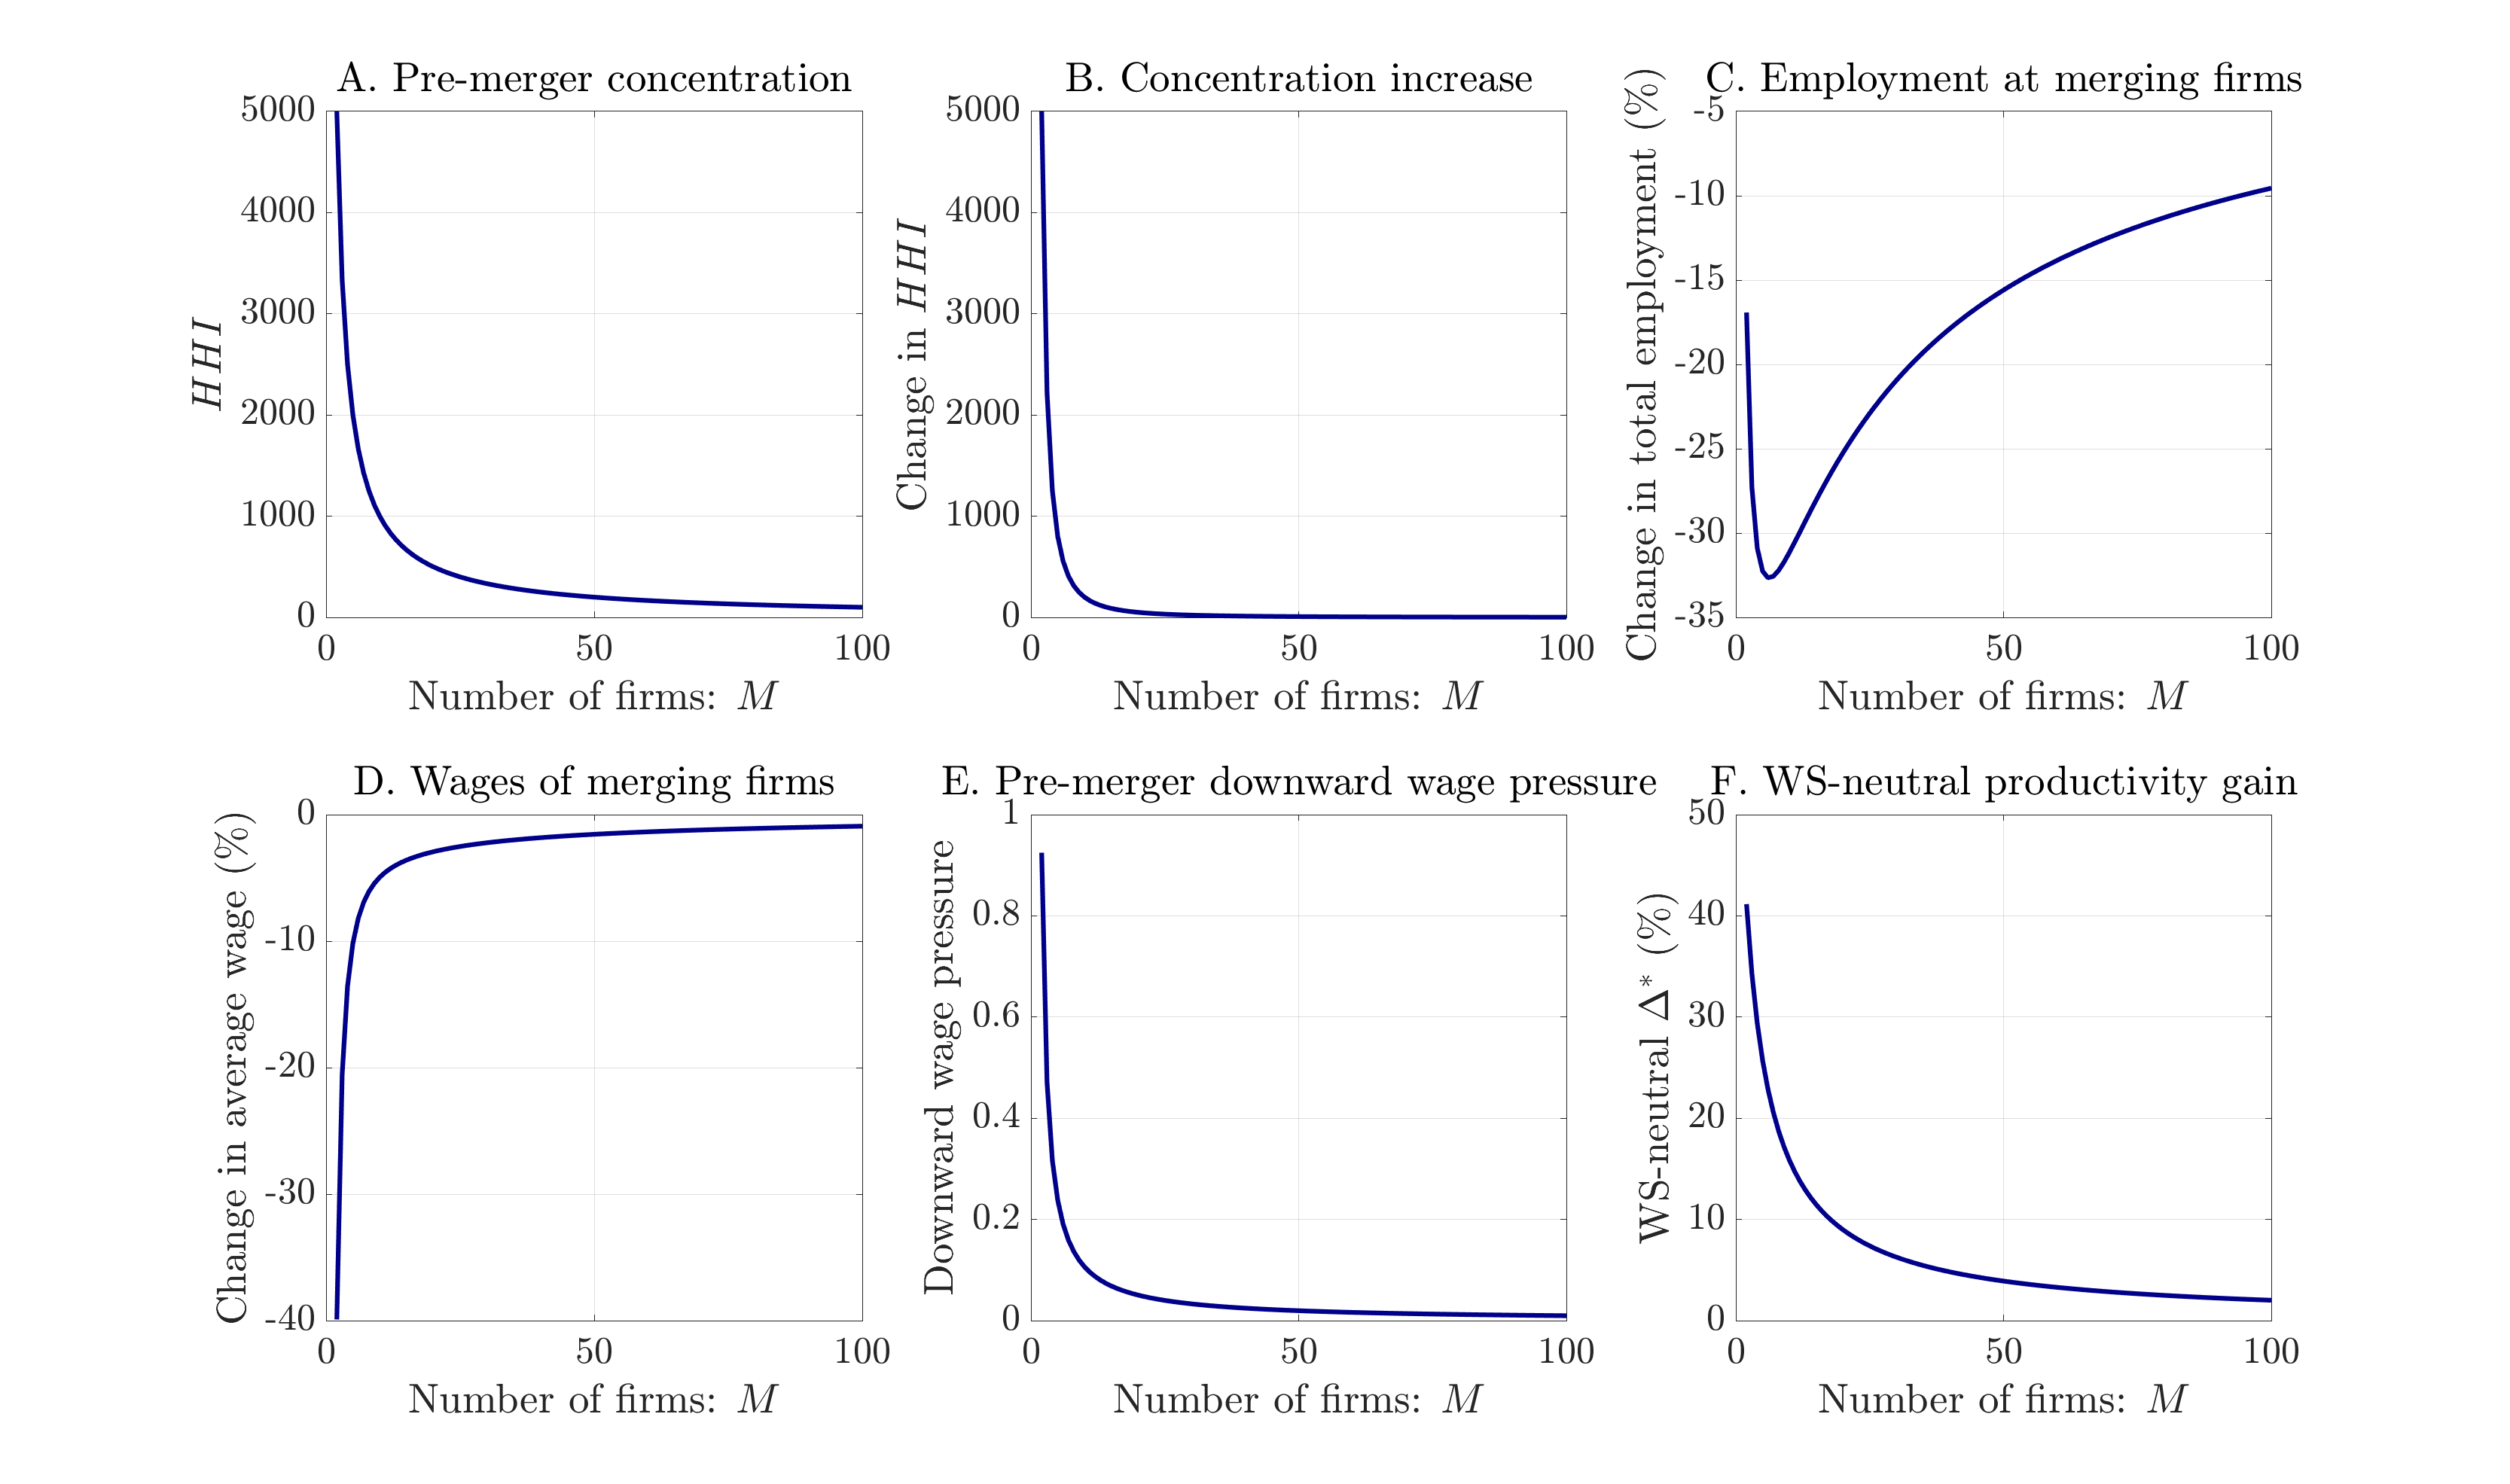
\includegraphics[width=18cm]{../results/figures/figb1_symmetric_mergers}
	\caption{Effects of symmetric mergers by firms-per-market $M_j$.}\label{fig:symmetric}
    \end{center}
\end{figure}

Figure \ref{fig:symmetric} shows how, in this simple example, the negative effects of a merger are much more pronounced in markets with initially fewer firms. 
We plot the effects on concentration, employment, wages, the diversion ratio, and the worker surplus neutral  productivity $\Delta^*$ defined in \emph{Proposition 2}.
Panel A shows that for $M_j=2$ concentration initially begins with a payroll Herfindahl of  $HHI_j=5,000$, corresponding to two identical and symmetric firms.\footnote{
    With two symmetric firms, $HHI_j=[(0.50\times 100)^2+(0.50\times 100)^2=5,000$.} 
Panel B shows that after the two symmetric firms merge, the Herfindahl reaches its maximum value of $HHI_j'=10,000$, implying a change in the Herfindahl of $\Delta HHI_j = HHI_j'-HHI_j=5000$. 
Panel C shows that this merger generates a 17 percent reduction in employment at the merging firms. 
In restricting quantities in this way, given the entity's new, higher level of market power, the monopsonist can \textit{lower} wages (Panel D).   
%\redSM{As described above, the diversion ratio describes how hiring at one firm increases overall marginal costs and reduces overall hiring [X] Make panel E DWP [X].}
Panel E plots the diversion ratio  (defined to be $-\frac{\partial n_{2j}}{\partial w_{1j}}/\frac{\partial n_{1j}}{\partial w_{1j}}$) and shows that it attains its highest value of 0.8 when duopsonists merge into a pure monopsonist.\footnote{Our model yields a convenient formula for diversion ratios as a function of parameters, shares and initial employment levels:
$$\text{Diversion ratio}=-\frac{\partial n_{2j}}{\partial w_{1j}}\left[\frac{\partial n_{1j}}{\partial w_{1j}}\right]^{-1}=\frac{\left(\eta-\theta\right)s_{1j}}{\left[\eta-\left(\eta-\theta\right)s_{1j}\right]}\left(\frac{n_{2j}}{n_{1j}}\right)$$.}  
A diversion ratio of 0.8 implies that for a hypothetical, partial equilibrium, wage hike sufficient to deliver one new worker to plant $i$, 0.8 workers leave plant $i'$. 

%Importantly, we structure our guidelines in Section \ref{sec:Guidelines} around the \emph{required efficiency gain} (REG), $\Delta^*$, that delivers either (i) worker surplus neutrality, (ii) output neutrality,  or (iii) employment neutrality. 
%We augment the merged firm's objective function with merger efficiency gains, $\Delta$, so that they solve
%\begin{equation}
%	\label{eq:pi_delta_augmented}
%	\pi_{ij} = \max_{n_{ij}, n_{i'j}}\:\: z_{ij} e^{\Delta}  n_{ij}  -w_{ij}n_{ij} +z_{i'j} e^{\Delta}  n_{i'j}  -w_{i'j}n_{i'j},
%\end{equation}
%subject to the labor supply curves for both $i$ and $i'$, given by \eqref{eq:n_inv}.

Panel F plots the post-merger \emph{required efficiency gain} (REG), $\Delta^*$,  required to deliver worker surplus neutrality (see Proposition 2). Following Proposition 2, we augment the merged firm's objective function with merger efficiency gains, $\Delta^*$, so that they solve
\begin{equation}
	\label{eq:pi_delta_augmented}
	\pi_{ij} = \max_{n_{ij}, n_{i'j}}\:\: z_{ij} e^{\Delta^*}  n_{ij}  -w_{ij}n_{ij} +z_{i'j} e^{\Delta^*}  n_{i'j}  -w_{i'j}n_{i'j},
\end{equation}
subject to the labor supply curves for both $i$ and $i'$, given by \eqref{eq:n_inv}. By definition of $\Delta^*$, the resulting employment and wage decisions of the newly merged firm yield constant sectoral wage and employment indexes, thus achieving worker surplus neutrality.

Panel F shows that when duopsonists merge into a pure monopsonist, the merge must yield efficiency gains of 40 percent in order for worker surplus neutrality. 
For markets with more than 35 identical firms, the REG for worker surplus neutrality lies below 5 percent, a commonly assumed value of merger efficiency gains \citep{farrell2010antitrust}. 

While Figure \ref{fig:symmetric} is a useful illustrative exercise, it is insufficient for merger analysis. 
In reality, firms within markets are not symmetric.  
Markets with 35 firms, like in the above example, may have three or four highly productive and relatively large firms while the remaining firms are small.
In practice, the market power accruing to these firms will be much more like that accruing to a firm in a market with five or six identically sized firms. 
A key contribution of our framework is to account for the across-market heterogeneity in the distribution of firms. 
Therefore, we next turn to our quantitative model.
Consistent with the data, in the quantitative model the average market has more than 100 firms, but the average $HHI$ is $1,100$. 
The latter is consistent with an $HHI$ that would be observed in a market with around 10 symmetric firms.
Comparing markets with 100 or 10 symmetric firms in Figure \ref{fig:symmetric}, required efficiency gains for worker surplus neutrality are enormously different.
%Accounting for where local labor markets lie between these extremes is therefore essential for calibrating merger policy.


%~~~~~~~~~~~~~~~~~~~~~~~~~~~~~~~~~~~~~~~~~~~~~~~~~~~~~~~~~~~~~~~~~~~~~~~~~~~~~~~~~~~~~~~~~~~~~~~~~~~~~~~~~~~~~~~~~
%~~~~~~~~~~~~~~~~~~~~~~~~~~~~~~~~~~~~~~~~~~~~~~~~~~~~~~~~~~~~~~~~~~~~~~~~~~~~~~~~~~~~~~~~~~~~~~~~~~~~~~~~~~~~~~~~~


\clearpage

\setcounter{table}{0} \setcounter{figure}{0} \renewcommand{\theequation}{C\arabic{equation}}
\renewcommand{\thetable}{C\arabic{table}} %
\renewcommand{\thefigure}{C\arabic{figure}}
\renewcommand{\thesubsection}{\thesection.\arabic{subsection}}


\section{Distribution of required efficiency gains}

 
In this section, we study the distribution of required efficiency gains for worker surplus neutrality. Similar to Section \ref{sec:Guidelines}, we simulate a representative set of mergers in the U.S. following the procedure outlined below: \vspace*{-.2cm}
{\small
\begin{enumerate}
	\item Draw $N=200,000$ markets from the empirical distribution of markets in the United States. This includes the number of firms, distributed $G(M_j)$, and the productivity of firms within each market, distributed $F(z_{ij})$.\vspace*{-.2cm}
	\item Randomly choose two candidate merging firms $i$ and $i'$. Only consummate the merger if $i$ and $i'$'s average pre-merger employment is greater than $\tilde{n}=46$. Imposing this size cutoff allows us to match the observed median merger size in \citet{Arnold}'s representative sample of mergers in the U.S. (see Section \ref{sec:validation} for additional details).\footnote{Note that the lower employment threshold of $\tilde{n}=46$ in this section is estimated so that the median pre-merger employment of the merging firms is 116. }
 \vspace*{-.2cm}
	\item Compute the REG for worker surplus neutrality, $\Delta^*$,  defined by Proposition 2.\vspace*{-.2cm}
	\item Index each REG, $\Delta^*$, by its simulation number $n\in\{1,\ldots,N\}$  and store the vector  $\{\Delta^*_n\}_{n=1}^N$.\vspace*{-.2cm}
	\item Compute moments of the distribution of  REGs, $\{\Delta^*_n\}_{n=1}^N$.\vspace*{-.2cm}
\end{enumerate}}

Figure \ref{fig:hhi_delta_hm} reports various moments of the distribution of REGs, $\{\Delta^*_n\}_{n=1}^N$.\footnote{
	Before moving on to the next figure, a notable feature of Figure \ref{fig:hhi_delta_hm} and subsequent figures,  is the missing cell values. 
	Mathematically, it is impossible to have certain combinations of $HHI$ and $\Delta HHI$ and certain target/acquirer shares. 
	To see this, notice that each component of $\Delta HHI_j= (s_{ij}+s_{i'j})^2-s_{ij}^2-s_{i'j}^2$ can be bound by the initial $HHI$. 
	Likewise shares are bound and must sum to less than one, $s_{i'j}+s_{ij}\leq 1$.  
	In competitive markets where $HHI\in[0,500)$, no merger between firms can produce a change in $HHI$ above a value of 50.}
%Since our aim is to parallel the existing horizontal merger guidelines provided by the \citet{doj2010guidelines}, we bin mergers based on their initial market concentration, $HHI_j=\sum_{i=1}^{M_j} s_{ij}^2$, as well as their (naive) change in concentration based on pre-merger shares, $\Delta HHI_j= (s_{ij}+s_{i'j})^2-s_{ij}^2-s_{i'j}^2$. 
Panel A reports the $20^{th}$ percentile of the REG distribution in each $\{HHI_j, \Delta HHI_j\}$ bin. 
Panel B reports the median value of the REG distribution in each $\{HHI_j, \Delta HHI_j\}$ bin.

\begin{figure}[t!]
	\centering
	\centering
	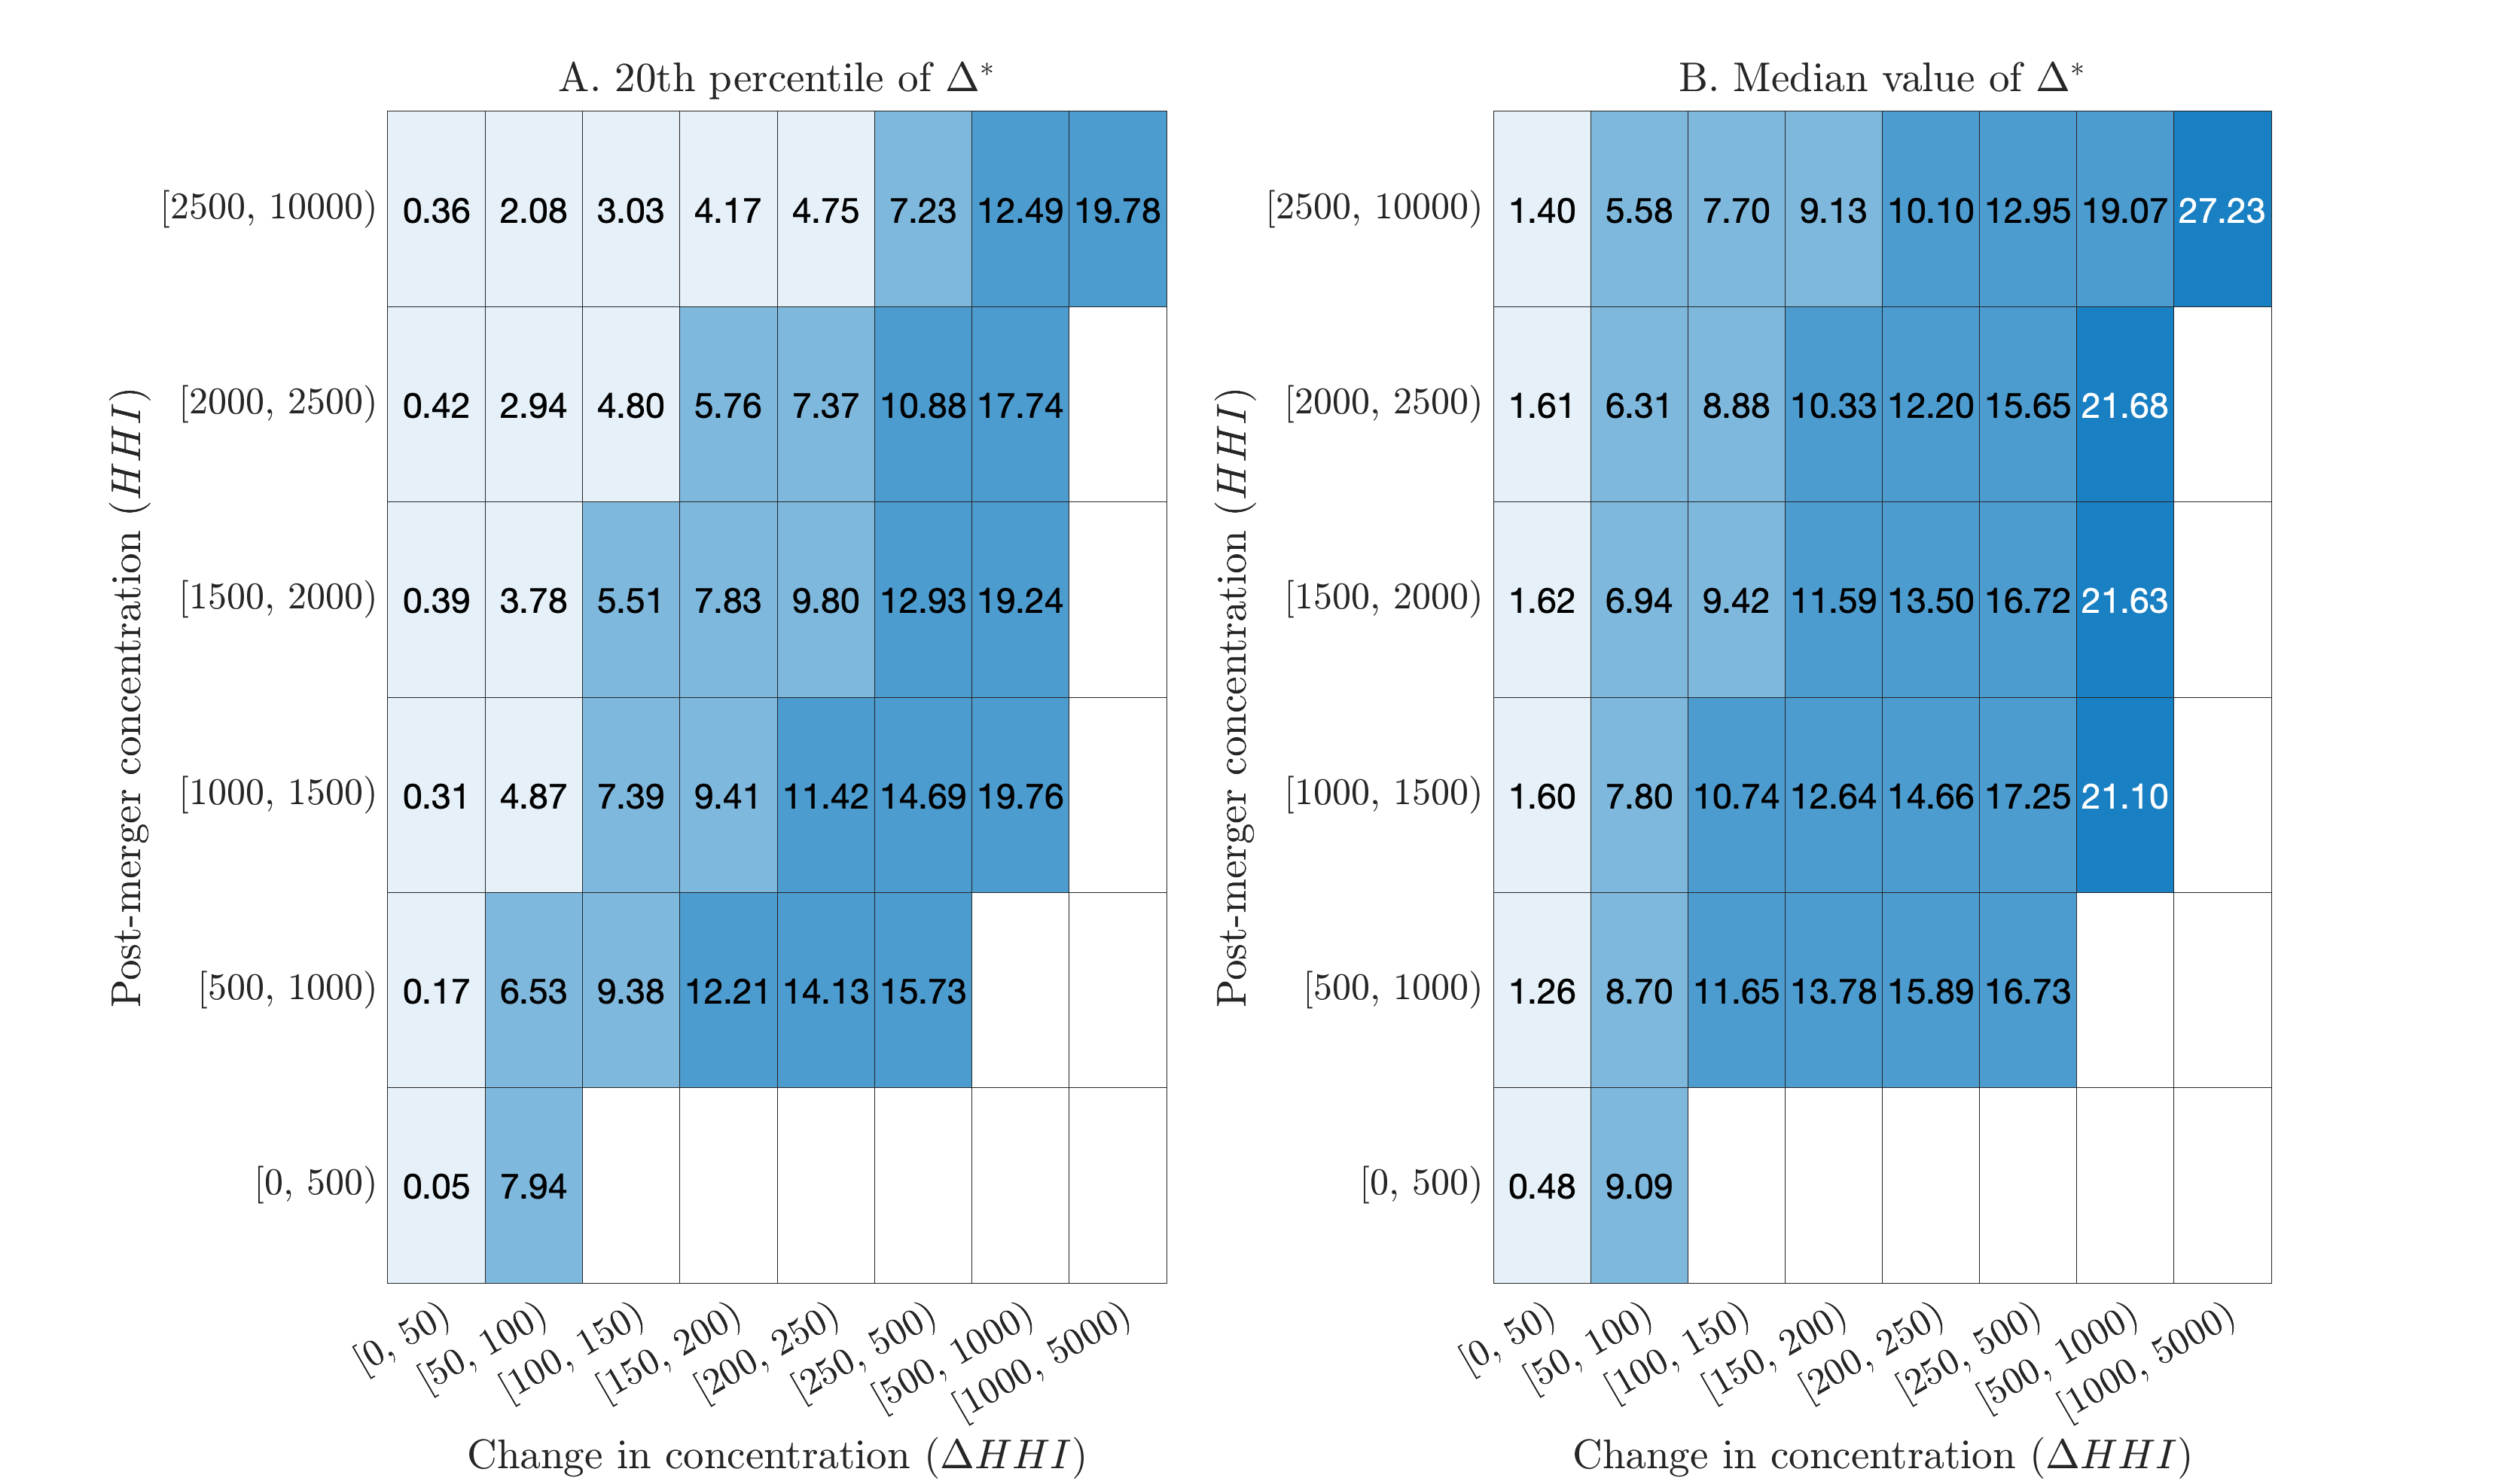
\includegraphics[width=18cm]{../results/figures/figC1_REGs_percentiles_heatmap.png}
	\caption{Percentiles of the distribution of worker surplus neutral efficiency gains $\{\Delta^*_n\}$}
	\label{fig:hhi_delta_hm}
\end{figure}

To interpret Figure \ref{fig:hhi_delta_hm}, consider the bottom left most cell of Panel A which corresponds to mergers in markets where $HHI_j\in[0,500)$ and $\Delta HHI_j \in [0,50)$. 
Within that cell, we have thousands of simulated mergers according to the procedure outlined above.  
The 20th percentile of the distribution of $\Delta_n^*$ within that cell is a 0.01 percent productivity gain. 
This can be interpreted in two ways. 
First, if presented with a merger with $HHI_j\in[0,500)$ and $\Delta HHI_j \in [0,50)$,  and merger efficiency gains are assumed to be 0.01 percent, then 80 percent of those mergers would yield worker surplus neutrality, or better. 
Second, if the regulator believed efficiency gains were near-zero and approved all mergers in which $HHI_j\in[0,500)$ and $\Delta HHI_j \in [0,50)$, the regulator would only mergers that harm workers 20 percent of the time. 
%Alternatively, among all simulated mergers where $HHI_j\in[0,500)$ and $\Delta HHI_j \in [0,50)$,  if merger efficiency gains are assumed to be 0.01 percent, 20 percent of permitted mergers would end up violating WS-neutrality and generate a worker surplus loss.

Panel A of Figure \ref{fig:hhi_delta_hm} shows that---holding initial concentration fixed---the 20th percentile of REGs monotonically increases in $\Delta HHI_j$.
 If merger efficiency gains are assumed to be 5 percent, \textit{less than} 20 percent of simulated mergers where $\Delta HHI_j >250$ generate a worker surplus gain. 
 In other words,  if merger efficiency gains are assumed to be 5 percent, \textit{more than} 80 percent of simulated mergers where $\Delta HHI_j >250$ generate a worker surplus loss. 
If merger efficiency gains are assumed to be 3 percent, \textit{more than} 80 percent of simulated mergers where $\Delta HHI_j >100$ generate a worker surplus loss. 
 
Panel B of Figure \ref{fig:hhi_delta_hm} reports the 50th percentile of required efficiency gains for worker surplus neutrality, $\{\Delta^*_n\}_{n=1}^N$, conditional on $HHI_j$ and $\Delta HHI_j$. 
Many of the qualitative and quantitative features of Panel B mirror Panel A.   
 If merger efficiency gains are assumed to be 5 percent, \textit{more than} 50 percent of simulated mergers where $\Delta HHI_j >50$ generate a worker surplus loss. 
 

We repeat this exercise and compute the distribution of required efficiency gains for worker surplus neutrality stratified by the merging firms' initial payroll shares of the local labor market.  Figure \ref{fig:shares_delta_hm}A plots the 20th percentile of the distribution of required efficiency gains $\{\Delta^*_n\}$ for worker surplus neutrality stratified by the merging firms' initial payroll shares of the local labor market. If efficiency gains are 5 percent, then less than 20 percent of mergers yield worker surplus gains in which the smaller merging firm's local payroll share is greater 5 percent. In other words, even if we assume a standard efficiency gain of 5 percent, more than 80 percent of mergers in which the smaller firm's payroll share of the local labor market is greater than 5 percent yield worker surplus losses. Likewise, Figure \ref{fig:shares_delta_hm}B reports the 50th percentile of the distribution of required efficiency gains. Even if efficiency gains are 6 percent (larger than the standard assumption), the majority of  mergers yield worker surplus losses if the smaller merging firm's local payroll share is greater 5 percent.



\begin{figure}
	\begin{center}
		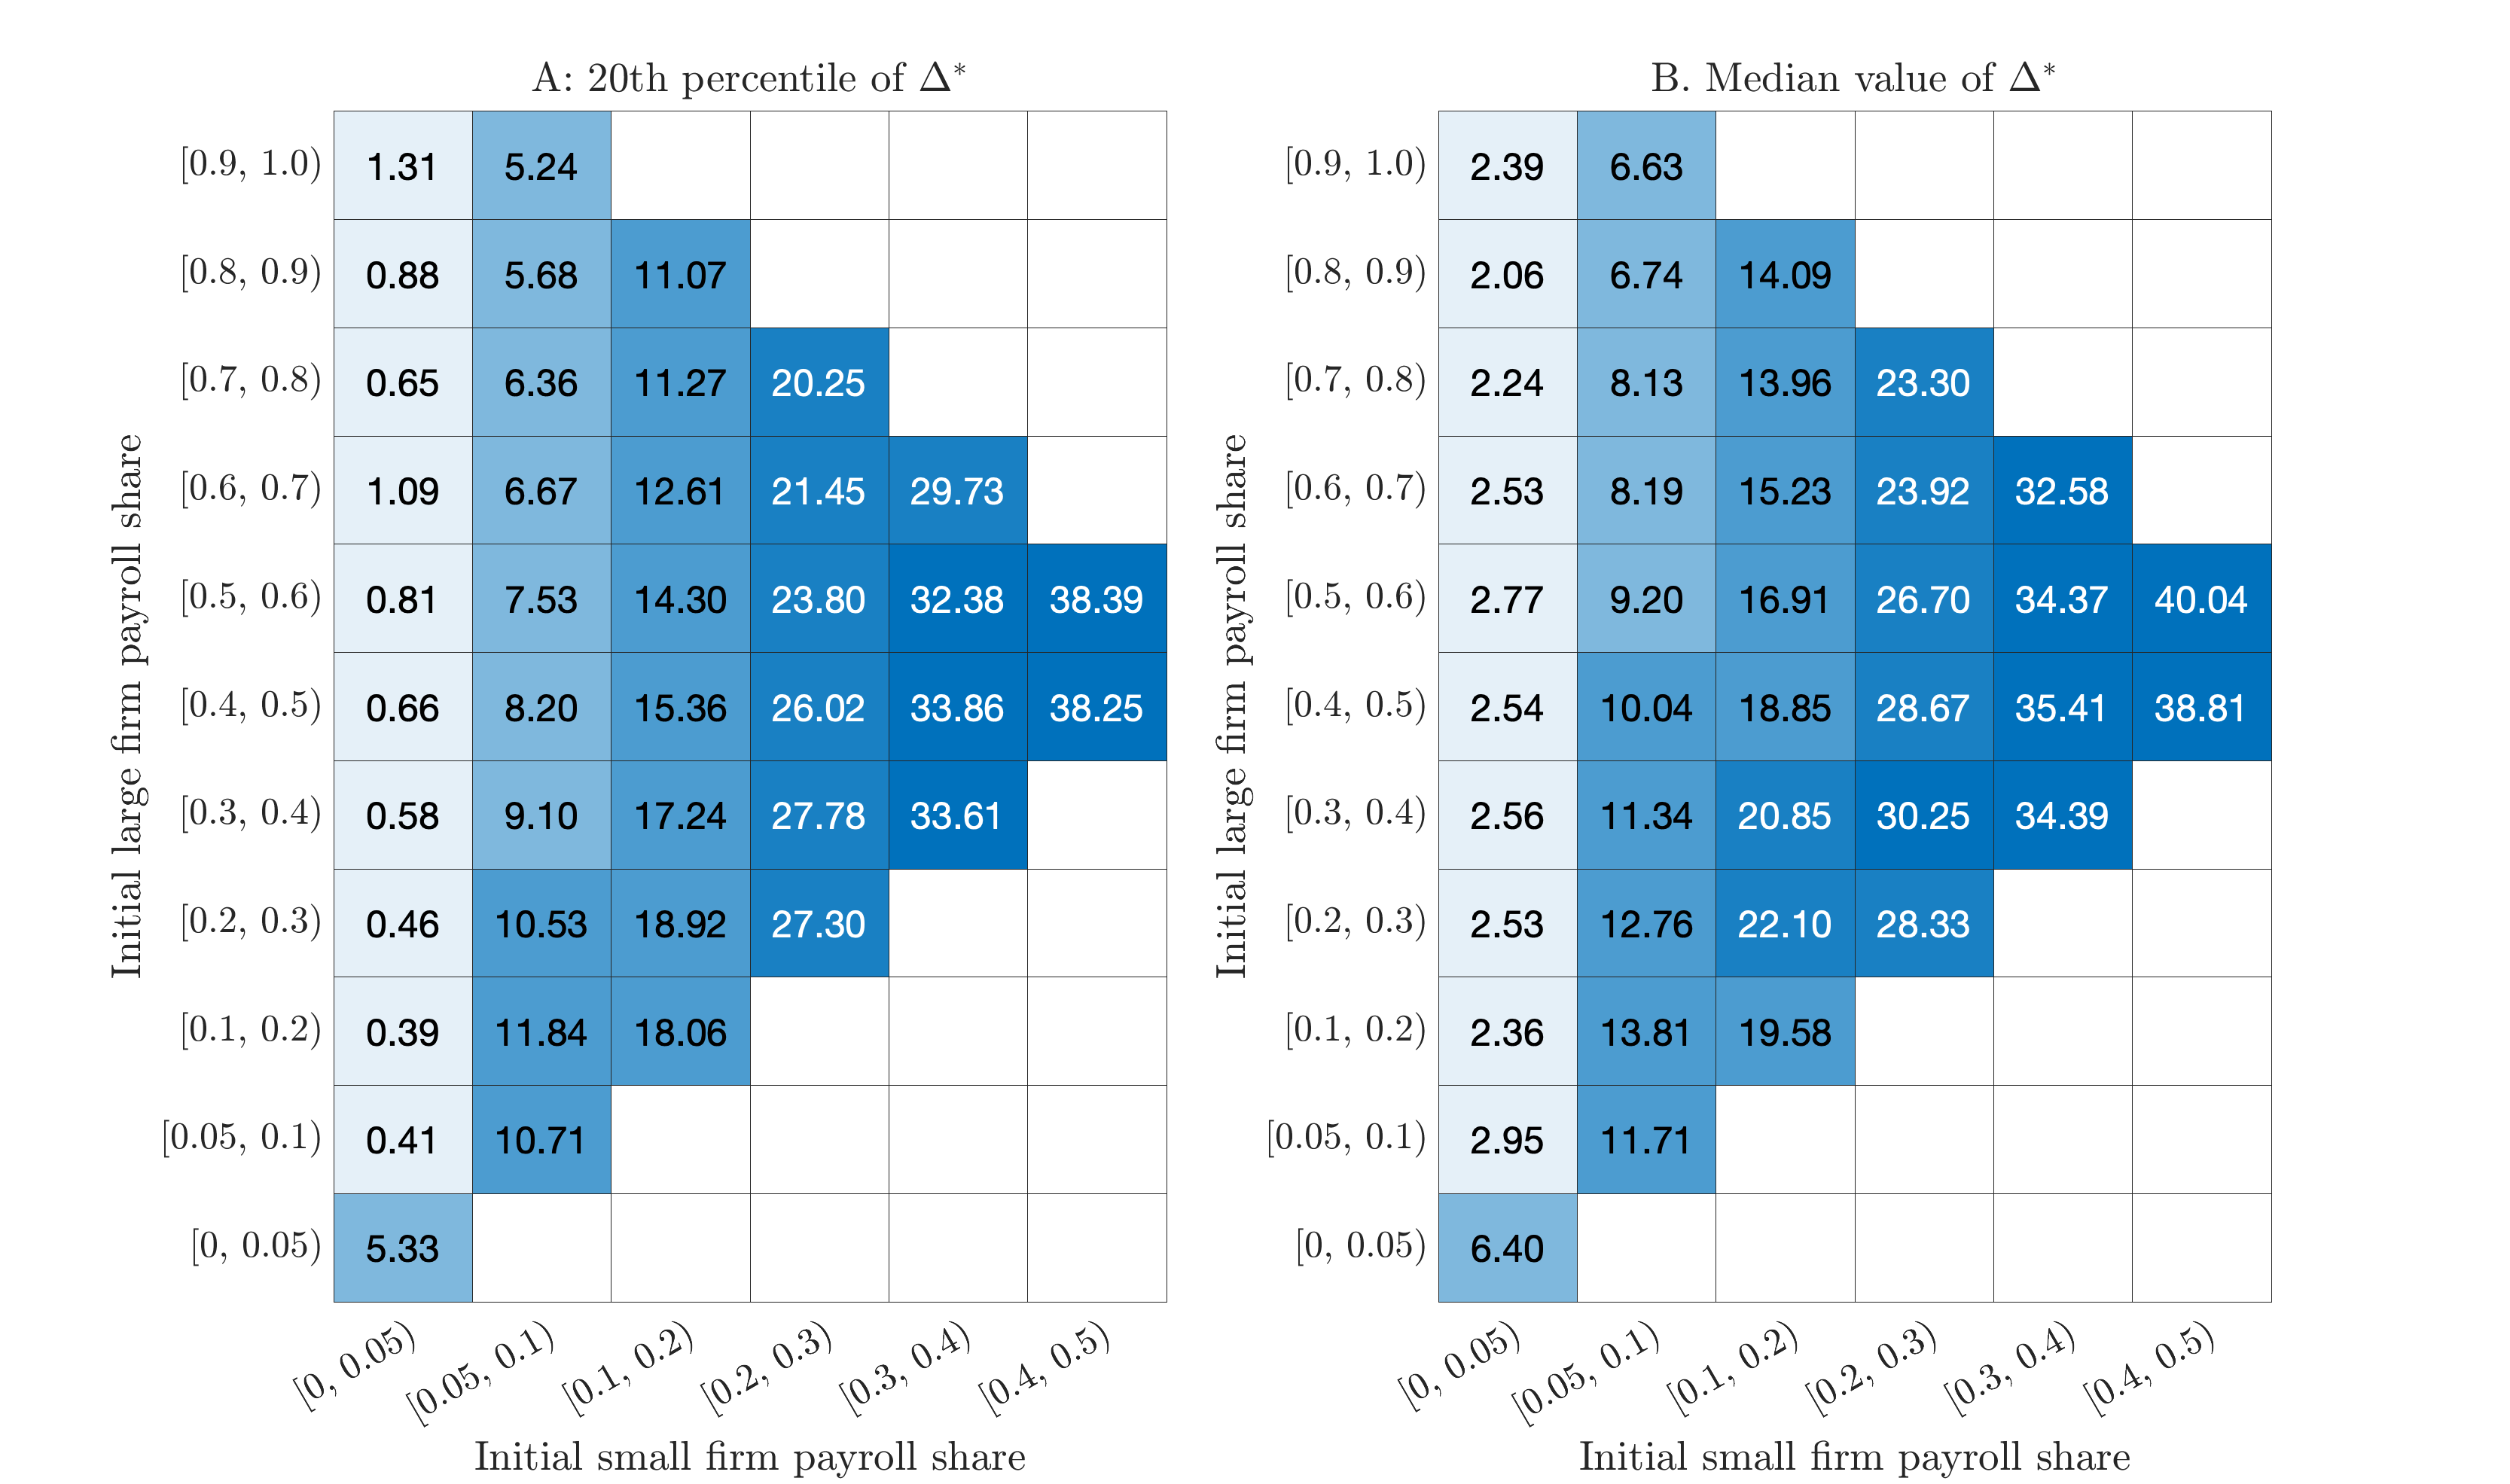
\includegraphics[width=18cm]{../results/figures/figC2_REGs_shares_heatmap}
		\caption{Percentiles of the distribution of required efficiency gains $\{\Delta^*_n\}$ for worker surplus neutrality - By shares}\label{fig:shares_delta_hm}
	\end{center}
\end{figure}



Figure \ref{fig:shares_cutoff_hm2} plots the fraction of mergers yielding worker surplus gains for efficiency gains of 5 percent (Panel A) and 10 percent (Panel B). Assuming a standard 5 percent efficiency gain, we find that if the smaller merging firm's local labor share is greater than 5 percent, less than 13 percent of all simulated mergers generate a worker surplus gain.  



\begin{figure}[h!]
	\begin{center}
		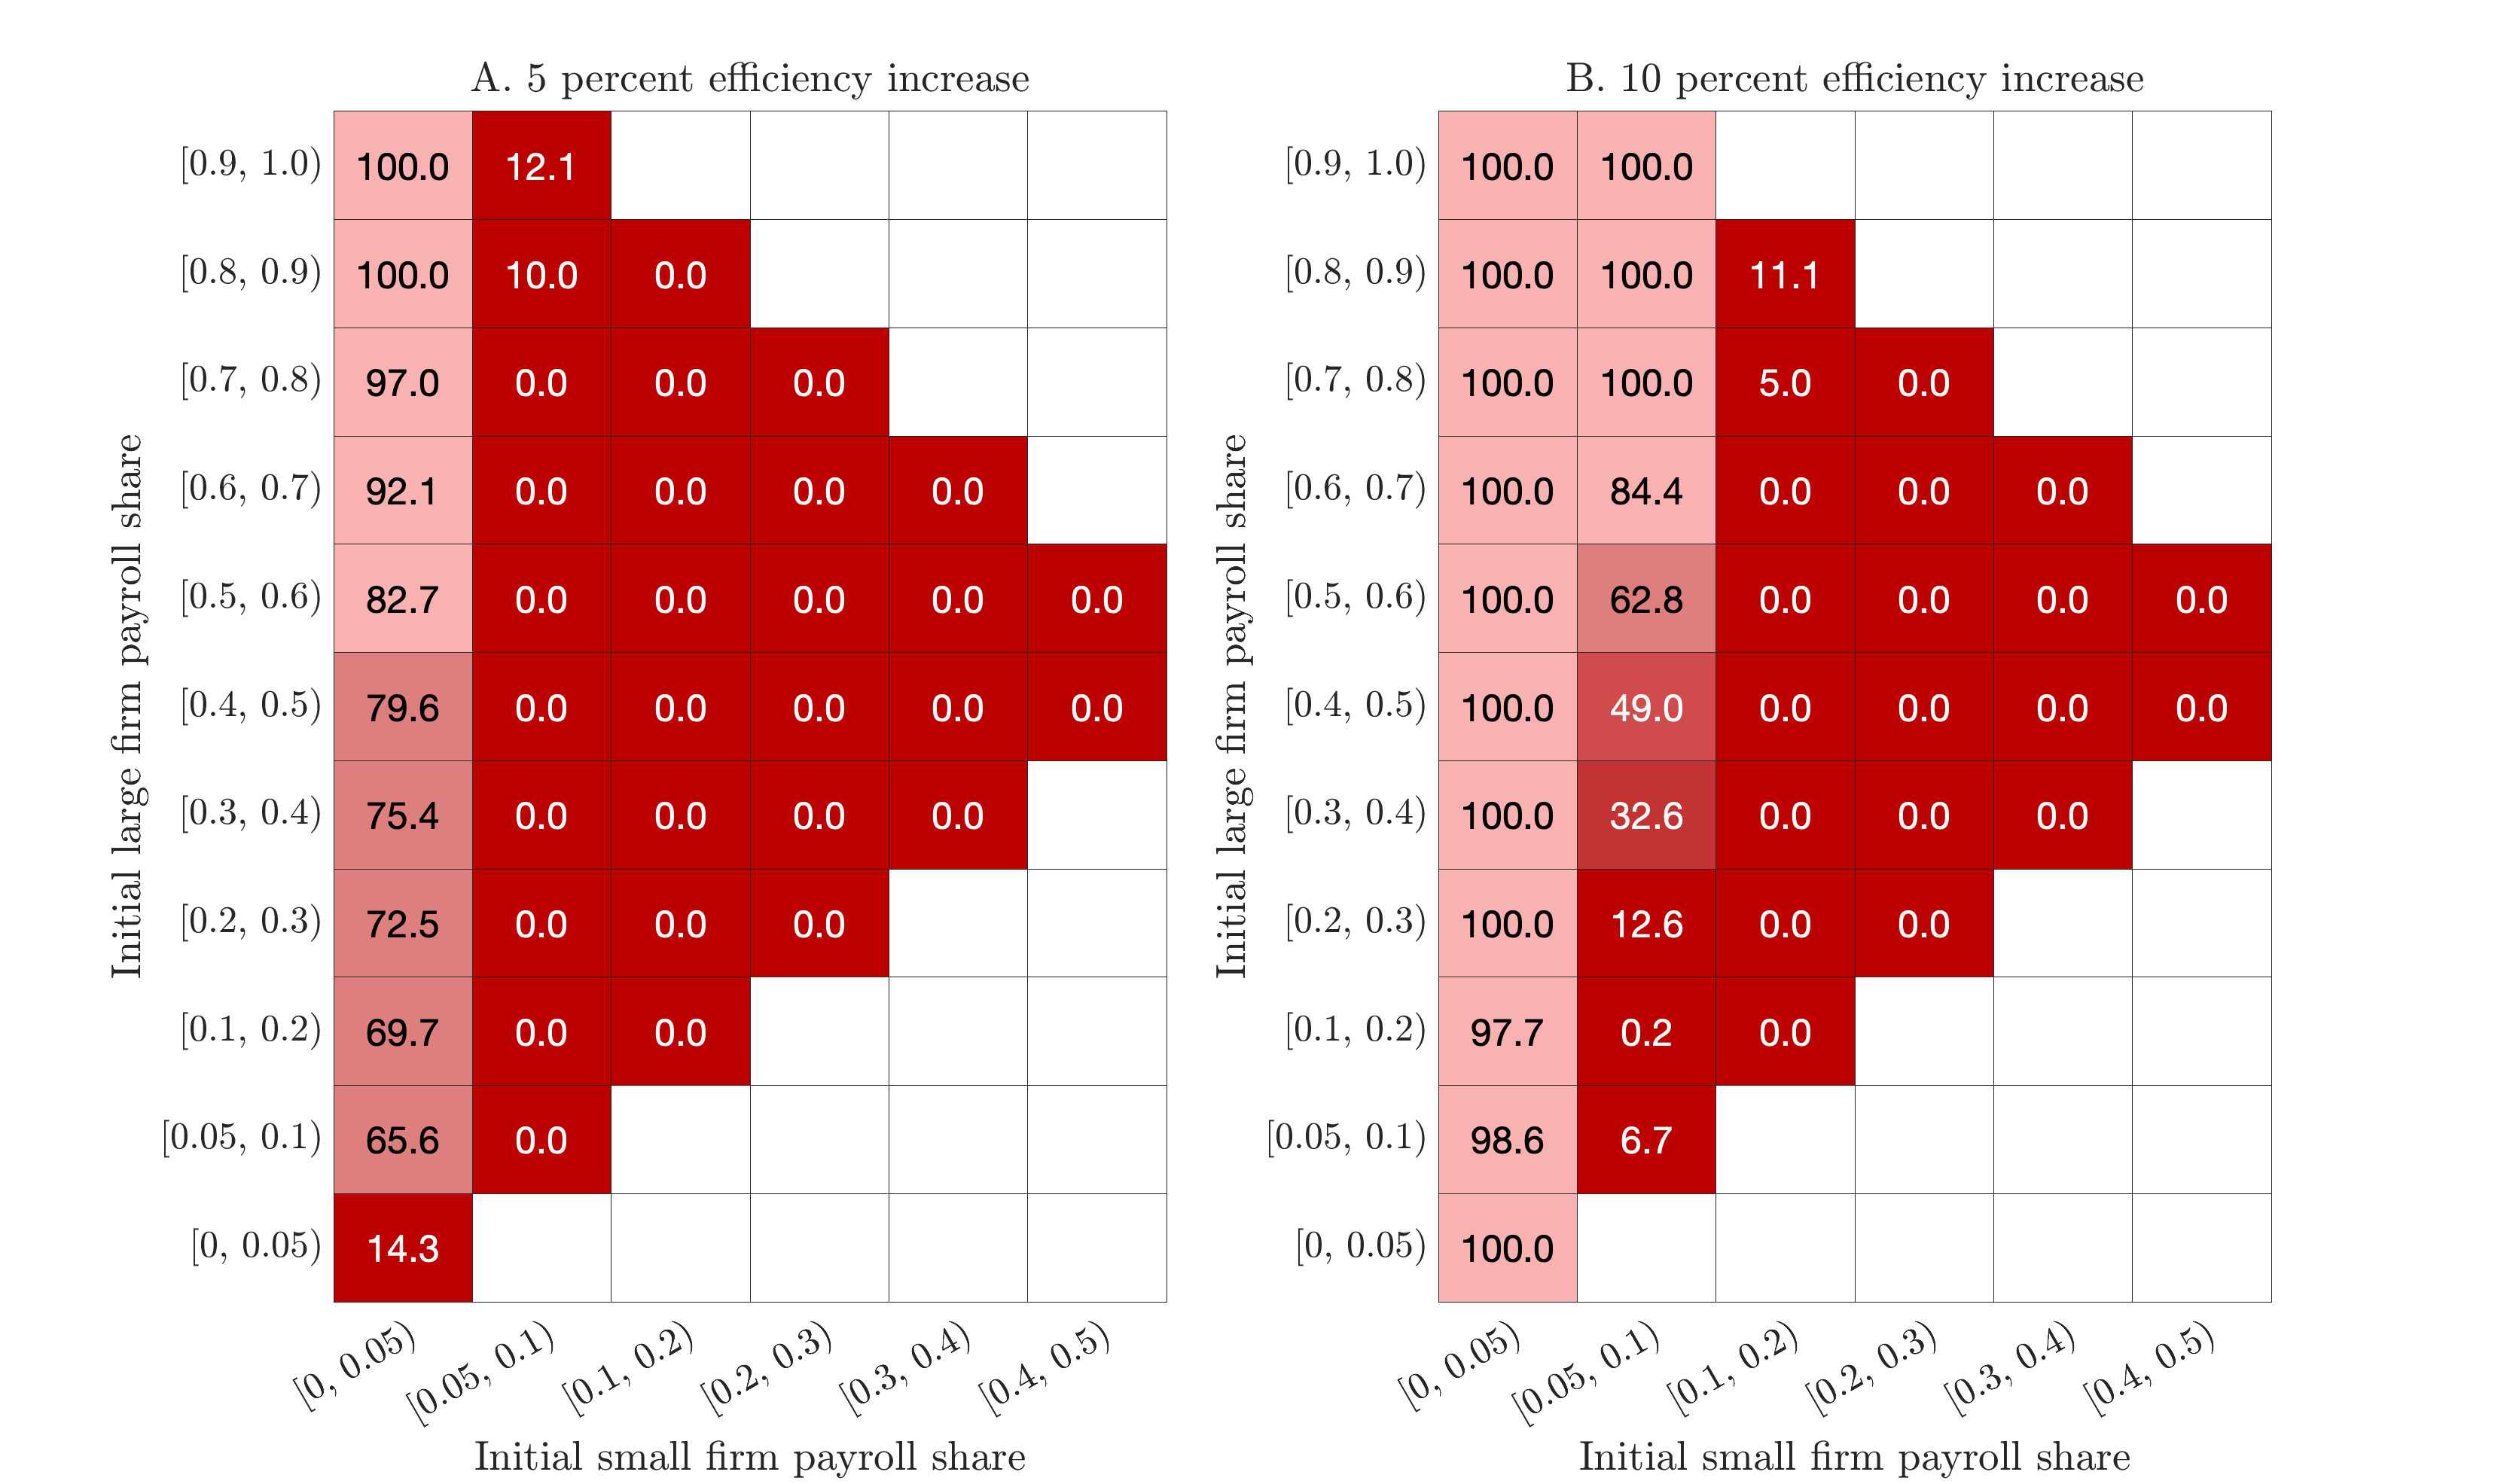
\includegraphics[width=18cm]{../results/figures/figC3_merger_fractions_heatmap}
		\caption{Fraction of mergers yielding worker surplus gains for efficiency gain $\Delta\in\{5\%,10\%\}$ - By shares}\label{fig:shares_cutoff_hm2}
	\end{center}
\end{figure}







\clearpage

\setcounter{table}{0} \setcounter{figure}{0} \renewcommand{\theequation}{D\arabic{equation}}
\renewcommand{\thetable}{D\arabic{table}} %
\renewcommand{\thefigure}{D\arabic{figure}}
\renewcommand{\thesubsection}{\thesection.\arabic{subsection}}

\section{Uni-dimensional merger guidelines}
\label{app:uni}
Next, we evaluate uni-dimensional merger guidelines  based on $HHI$s alone or $\Delta HHI$'s alone and applied to our simulated $N=200,000$ representative mergers.  


Figure \ref{fig:hhi_rules}  plots the expected change in the market-level wage index under the assumption of various uni-dimensional merger guidelines.
The $x$-axis varies the assumed level of efficiency gains  from 0 to 15 percent. 
Each line corresponds to a different  uni-dimensional merger guideline.

Figure \ref{fig:hhi_rules}A shows that under an assumed efficiency gain of 0 percent (light-blue, triangles), allowing mergers yields an average market-level wage reduction of -2.4 percent. 
Merging firms cut employment to lower wages, and thus the mergers are not worker surplus neutral. 
Keeping the assumed efficiency gain at 0 percent and moving up to the next darkest line (circles), we see that a policy in which all mergers are blocked in extremely concentrated markets $(HHI_j>5,000)$ mitigates the average market-level wage loss to -1.7 percent.
The expected drop in the wage index is mitigated because mergers with the largest negative impact on wages are now blocked.
 
If a regulator aims to have an expected zero decline in wages, and assumes a 5 percent efficiency gain, then Figure \ref{fig:hhi_rules}A shows that a policy of blocking mergers with an $HHI>1,500$ is necessary. 
 

Figure \ref{fig:hhi_rules}B yields a similar set of results for $\Delta HHI$ thresholds. If a regulator aims to have an expected zero decline in wages, and assumes a 5 percent efficiency gain, then Figure \ref{fig:hhi_rules}A shows that a policy of blocking mergers with an $\Delta HHI>300$ would need to be implemented. 


\begin{figure}[t!]
	\begin{center}
	\hspace*{-.5cm}\includegraphics[width=18cm]{../results/figures/figD1_unidimensional}
	\caption{Expected change in market wage under alternative merger policies}\label{fig:hhi_rules}\vspace*{-.3cm}
    \end{center}
    \footnotesize{\underline{Notes}:
    Figures plots the Expected change in market-level wage $\mathbf{W}_j$ post-merger as a function of the assumed efficiency gain and merger policy. Efficiency gain on the x-axis is applied to both merging plants in all cases.
    }
\end{figure}

\subsection{Confidence levels}
\label{app:confidence}


Table \ref{tab:hhi_cutoffs} reports the necessary uni-dimensional $HHI$ and $\Delta HHI$ thresholds necessary to guarantee a certain fraction of approved mergers yield a worker surplus gain. 



\begin{table}[ht!]
\centering
\resizebox{1\width}{!}{\begin{tabular}{lcccccc}
\toprule
 & \multicolumn{5}{c}{\textbf{Probability of WS gain}} \\ 
 & 30$\%$ & 35$\%$ & 40$\%$ & 45$\%$ & 50$\%$ \\ 
\midrule
\multicolumn{6}{l}{\textbf{HHI}} \\ 
1$\%$ Efficiency gain & 1694 & 1313 & 1049 &  863 &  726\\ 
2$\%$ Efficiency gain & 3524 & 2301 & 1734 & 1372 & 1107\\ 
3$\%$ Efficiency gain & 9990 & 4150 & 2643 & 1959 & 1548\\ 
4$\%$ Efficiency gain & 10000 & 9990 & 4316 & 2800 & 2086\\ 
5$\%$ Efficiency gain & 10000 & 10000 & 9990 & 4316 & 2878\\ 
\midrule
\multicolumn{6}{l}{\textbf{$\Delta$ HHI}} \\ 
1$\%$ Efficiency gain &  140 &   80 &   55 &   40 &   30 \\ 
2$\%$ Efficiency gain &  751 &  305 &  170 &  105 &   75 \\ 
3$\%$ Efficiency gain & 4850 & 1066 &  440 &  240 &  150 \\ 
4$\%$ Efficiency gain & 5000 & 4645 & 1156 &  511 &  285 \\ 
5$\%$ Efficiency gain & 5000 & 5000 & 4209 & 1176 &  556 \\ 
\bottomrule 
\end{tabular}}
\caption{Uni-dimensional $HHI$ and $\Delta HHI$ cutoffs necessary so that $\{30\%,35\%,40\%,45\%,50\%\}$ of mergers yield a worker surplus gain.  \label{tab:hhi_cutoffs}}
\end{table}



\clearpage




\section{Output-based merger guidelines} 
\label{app:output}
We provide output-based guidance on mergers in Figure \ref{fig:output_losses}. In this section, we simulate a random set of mergers from all pairwise combinations of firms, and -- unlike the main text --  we consummate all mergers regardless of firm size: \vspace*{-.2cm}
{\footnotesize
\begin{enumerate}
	\item Draw $N=200,000$ markets from the empirical distribution of markets in the United States. This includes the number of firms, distributed $G(M_j)$, and the productivity of firms within each market, distributed $F(z_{ij})$.\vspace*{-.2cm}
	\item Randomly choose two candidate merging firms $i$ and $i'$. In this section -- unlike the main text --  we consummate all mergers regardless of employment. 
 \vspace*{-.2cm}
	\item Compute the probability of an output loss from the merger, and if the merger results in a loss, compute the magnitude of the output. \vspace*{-.2cm}
\end{enumerate}}




Panel A shows the fraction of simulated mergers that yield an output loss \emph{at the market level} for a given level of efficiency gain $\Delta$ in equation \eqref{eq:pi_delta_augmented}. 
When the merging firms' combined pre-merger payroll shares are less than 20 percent and the efficiency gains from the merger are assumed to be 5 percent, all simulated mergers generate output gains. 
That is, a 5 percent efficiency gain more than offsets the output losses due to the merging firms contracting employment. 
%If merging firms' combined initial shares are around 0.60 (as in the case of PRH and Simon \& Schuster),
%then only 50 percent of mergers have output gains if productivity is assumed to increase at both firms by 5 percent.
%When assumed efficiency gains are 10 percent, losses occur when the combined merging firms' payroll shares exceed 60 percent.


Panel B shows the median output loss conditional on the merger generating an output loss. 
If the efficiency gain from a merger is 5 percent, the median total market-level output loss from a merger is upwards of 2 percent whenever the combined merging firms' payroll shares exceed 60 percent. 
\begin{figure}[h!]
	\begin{center}
		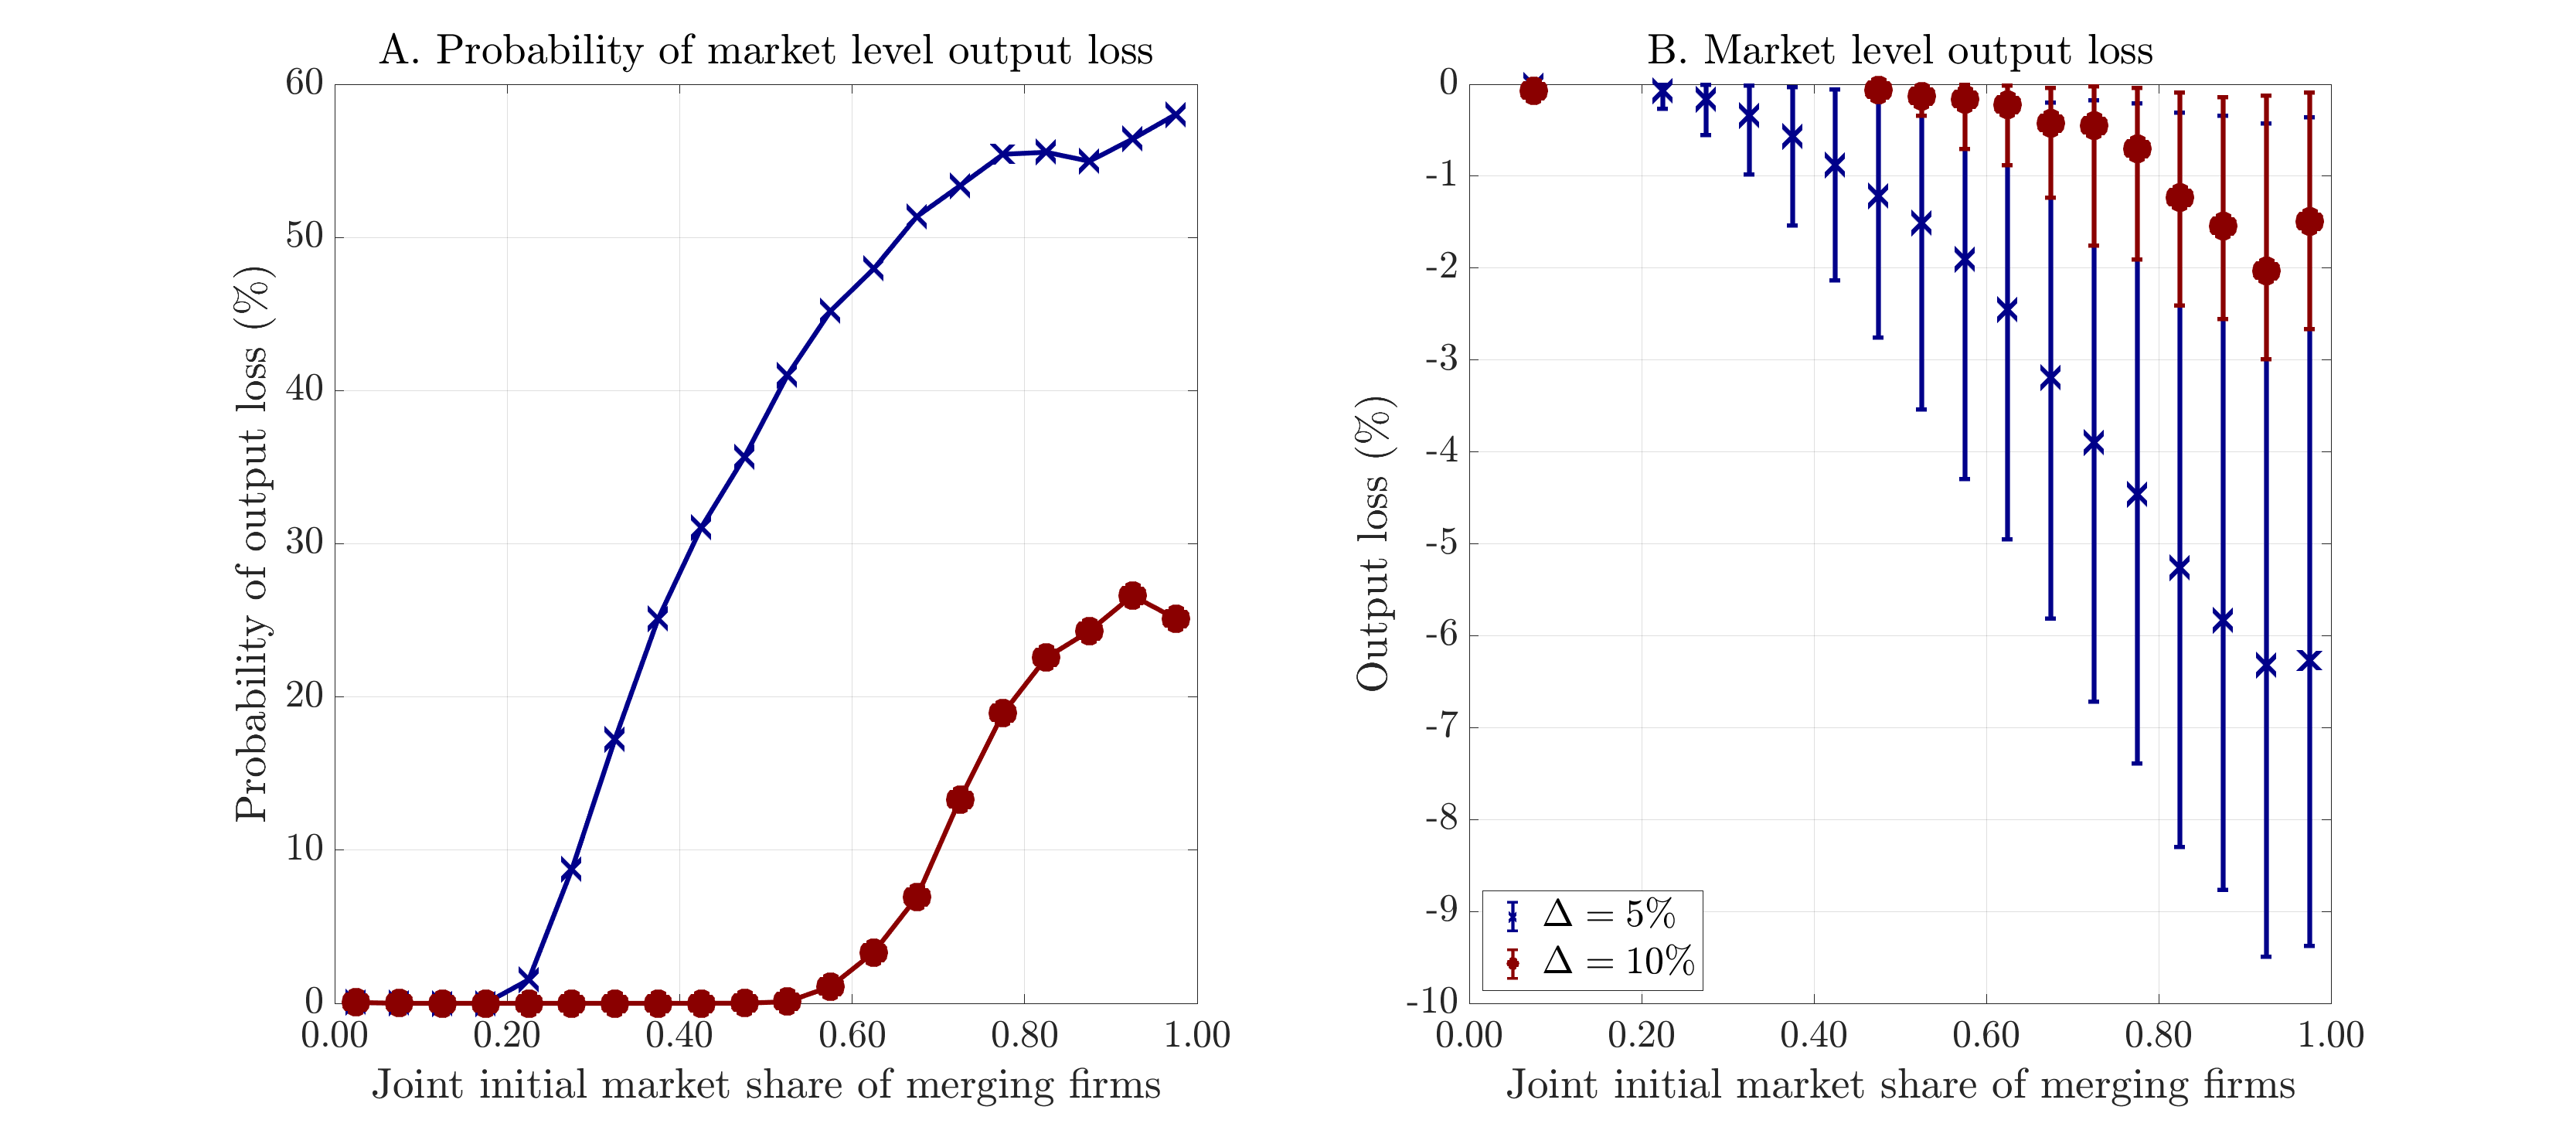
\includegraphics[width=18cm]{../results/figures/figd2_output_losses}
		\caption{Output losses for a merger efficiency gain of $\Delta^+\in\{5\%,10\%\}$}\label{fig:output_losses}
		\vspace*{.5cm}
	\end{center}
 
\end{figure}
\clearpage  

\section{Employment-based merger guidelines}
\label{app:emp}
Following the same procedure in Appendix \ref{app:output}, Figure \ref{fig:employment_losses}A plots the probability that a merger generates an employment loss, and if there is an employment loss, Figure \ref{fig:employment_losses}B computes the magnitude of that loss.
Since productivity gains increase output, conditional on employment, employment losses are larger and more significant than output losses, even for smaller mergers. 
When merging firms' payroll shares are above 20 percent, even if efficiency gains are 5 percent, a majority of our simulated mergers generate employment losses at the market level (i.e. taking into account reallocation of workers to other firms in the market). 
Panel B shows the median employment loss at the market level, conditional on the merger generating an employment loss. 
If efficiency gains are 5 percent, the median employment loss is upwards of 1 percent whenever the combined merging firms' payroll shares exceed 30 percent. 
Greater efficiency gains from mergers are required to mitigate employment losses than output losses.

\begin{figure}[h!]
 
	\begin{center}
		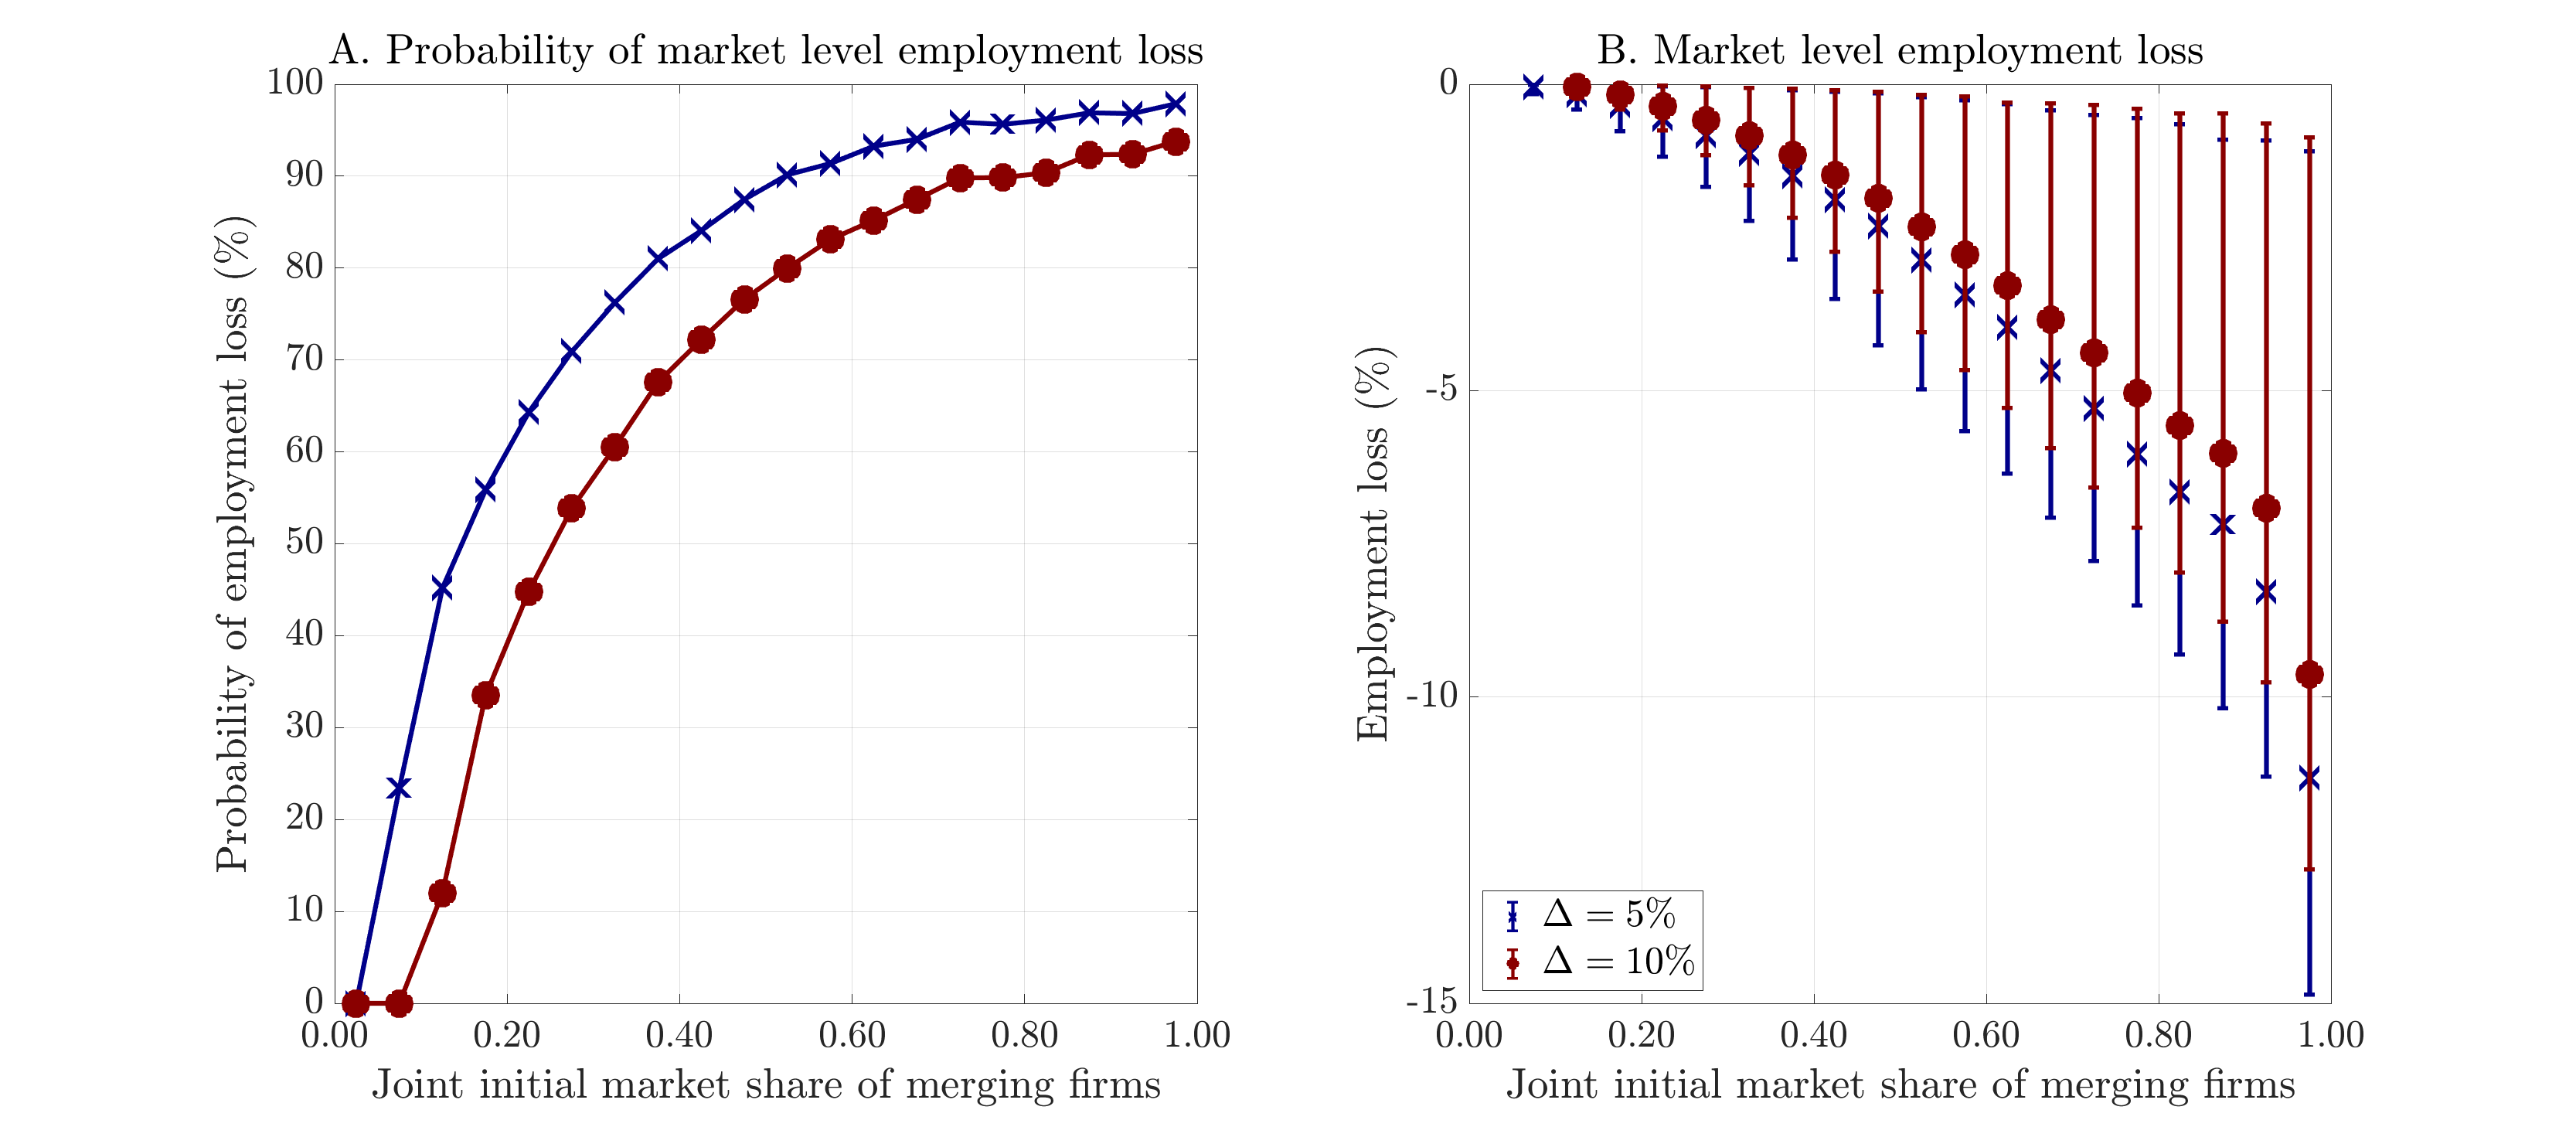
\includegraphics[width=18cm]{../results/figures/figd3_employment_losses}
		\caption{Employment losses for a merger efficiency gain of $\Delta^+\in\{5\%,10\%\}$}\label{fig:employment_losses}
	\end{center}
\end{figure}
\clearpage 
%
%\section{Additional Results on the Penguin Random House Merger}
%\label{app:prh_appendix}
%
%\begin{figure}[t!]
%	\begin{center}
%	\includegraphics[width=11cm]{img/prh_firmlevel.eps}
%	\caption{Expected change in wages in Penguin-Random-House \& Simon-Schuster merger}\label{fig:prh_firmlevel}\vspace*{-.3cm}
%    \end{center}
%    \footnotesize{
%    \underline{Notes}:
%    Figures plots the merger-induced changes in wages at PRH and SS as a function of the assumed efficiency gain. The market structure mimics the \textit{Penguin Random House} (PRH) and \textit{Simon \& Schuster} (SS) merger case based on  Exhibit 963 \citep[][p. 27]{penguin2022}.  The efficiency gain on the x-axis is applied to both merging plants as defined by equation \eqref{eq:pi_delta_augmented}. 
%    } 
%\end{figure}
%
%Panel A in Figure \ref{fig:prh_firmlevel} plots the change in the wage offered by Penguin Random House for various efficiency gains following a merger in the publishing market. Without any efficiency gain, the PRH and SS merger reduces PRH wages by approximately $4.5$ percent. The efficiency gains required for workers at PRH to earn the same wage as before the merger is 10\%. In comparison, the government witness in the judicial option \citep[][p. 57]{penguin2022} estimated wage losses at PRH of $3.7-7.4$ percent.
%
%Panel B in Figure \ref{fig:prh_firmlevel} plots the change in the wage offered by Simon \& Schuster. Without any efficiency gain, the PRH and SS merger reduces wages at SS by approximately $26$ percent. The efficiency gains required for workers at SS to earn the same wage as before the merger is $55$ percent. In comparison, the government witness in the judicial option \citep[][p. 57]{penguin2022} estimated wage losses at SS of $6.4-19.2$ percent.
%
%
%Why are our wage losses larger? The expert in the case adopted a second-price auction.\footnote{See the expert's slides here: \url{https://www.justice.gov/d9/case-documents/attachments/2022/08/08/408636.pdf}} The optimal strategy is to bid one's true value. So competitors' bids do not respond to the PRH/SS merger, i.e. the 2nd/4th/5th etc. largest publishing houses have some exogenous values of winning the auction and they continue to bid those values. In our model, however, we have competitors cutting wages.
%
%Since wages are strategic complements in our model, when the competitors cut wages, that feeds back into merging firms cutting wages further. There is much evidence for such spillovers (\citet{Staiger2010}, \citet{engbom2017earnings} among others), and so we believe our framework is a better approximation of what would have transpired had PRH and SS merged.

\section{Welfare approximation}
\label{app:welfare}


 Table \ref{tab:merger_guidelines_welfare} reports the welfare implications of various merger guidelines. We derive these welfare metrics as follows. We assume that mergers occur in a positive measure $\overline{J}$ of  identical markets, where we organize market indexes such that  $j\in[0,\overline{J}]$ markets are involved in the merger. We use a first-order Taylor expansion to approximate the welfare effects: 
\begin{scriptsize}
\begin{equation*}
\begin{aligned}
U\left(\mathbf{C},\mathbf{N}\right) \approx U\left(\mathbf{C}_{0},\mathbf{N}_{0}\right) &+\left[\frac{d}{dC}U\left(\mathbf{C},\mathbf{N}\right)\frac{d\mathbf{C}}{d\mathbf{W}\mathbf{N}}\frac{d\mathbf{W}\mathbf{N}}{d\int_{0}^{\overline{J}}\mathbf{W}_{j}\mathbf{N}_{j}dj}\right]\Bigg|_{\mathbf{C}=\mathbf{C}_{0},\mathbf{N}=\mathbf{N}_{0}}\underbrace{d\int_{0}^{\overline{J}}\mathbf{W}_{j}\mathbf{N}_{j}dj}_{\text{merger induced}} +\left[\frac{d}{d\mathbf{N}}U\left(\mathbf{C},\mathbf{N}\right)\frac{d\mathbf{N}}{d\int_{0}^{\overline{J}}\mathbf{N}_{j}^{\frac{\theta+1}{\theta}}dj}\right]\Bigg|_{\mathbf{C}=\mathbf{C}_{0},\mathbf{N}=\mathbf{N}_{0}}\underbrace{d\int_{0}^{\overline{J}} \mathbf{N}_{j}^{\frac{\theta+1}{\theta}}dj}_{\text{merger induced}}
\end{aligned}
\end{equation*}
\end{scriptsize}
The household budget constraint is given by
\begin{footnotesize}
\begin{equation*}
\begin{aligned}
    \mathbf{C}  & =  	  \int_0^1 \mathbf{W}_{j} \mathbf{N}_{j} dj
\end{aligned}
\end{equation*}
\end{footnotesize}
Thus, we can compute
\begin{footnotesize}
\begin{equation*}
\begin{aligned}
\frac{d\mathbf{C}}{d\mathbf{W}\mathbf{N}} = 1, \qquad \frac{d\mathbf{W}\mathbf{N}}{d\int_{0}^{\overline{J}}\mathbf{W}_{j}\mathbf{N}_{j}dj} = 1.
\end{aligned}
\end{equation*}
\end{footnotesize}
Next, we use a first-order Taylor approximation to approximate aggregate labor supply $\mathbf{N}$:
\begin{footnotesize}
\begin{equation*}
\begin{aligned}
    \mathbf{N}  =  \left[\int_0^1 \mathbf{N}_{j}^{\frac{\theta+1}{\theta}}dj\right]^{\frac{\theta}{\theta+1}}  
                \approx \mathbf{N}_{0} + \frac{\theta}{\theta+1} \mathbf{N}_{0}^{-\frac{1}{\theta}} \left(\int_{0}^{1} \left(\mathbf{N}_j^{\frac{\theta + 1}{\theta}} - \mathbf{N}_0^{\frac{\theta + 1}{\theta}}\right) dj\right).
\end{aligned}
\end{equation*}
\end{footnotesize}
Thus, we can compute the derivative of $\mathbf{N}$ with respect to the contribution of market $j$ to $\mathbf{N}$: 
\begin{footnotesize}
\begin{equation*}
\begin{aligned}
\frac{d\mathbf{N}}{d\int_{0}^{\overline{J}}\mathbf{N}_{j}^{\frac{\theta+1}{\theta}}dj} = \frac{\theta}{\theta+1} \mathbf{N}_{0}^{-\frac{1}{\theta}}.
\end{aligned}
\end{equation*}
\end{footnotesize}
%Preferences are GHH and are given by
%\begin{footnotesize}
%\begin{equation*}
%\begin{aligned}
%U(\mathbf{C},\mathbf{N}) = \mathbf{C} - \bar{\psi}^{-\frac{1}{\psi}} \frac{\mathbf{N}^{1+\frac{1}{\psi}}}{1 + \frac{1}{\psi}}. 
%\end{aligned}
%\end{equation*}
%\end{footnotesize}
With the GHH preferences in the main text, the marginal utility of consumption and marginal disutility of labor evaluated at the pre-merger levels of $\mathbf{C}$ and $\mathbf{N}$ are 
\begin{footnotesize}
\begin{equation*}
\begin{aligned}
    &\frac{d}{d\mathbf{C}} U(\mathbf{C}, \mathbf{N})\Big|_{\mathbf{C}=\mathbf{C}_{0},\mathbf{N}=\mathbf{N}_{0}} = 1, \qquad \frac{d}{d\mathbf{N}} U(\mathbf{C}, \mathbf{N})\Big|_{\mathbf{C}=\mathbf{C}_{0},\mathbf{N}=\mathbf{N}_{0}} = -\bar{\psi}^{-\frac{1}{\psi}} \mathbf{N}_0^{\frac{1}{\psi}}.
\end{aligned}
\end{equation*}
\end{footnotesize}
Then, welfare following a merger in a market with measure $[0,\overline{J}]$ is approximated by
\begin{footnotesize}
\begin{equation}
\begin{aligned}
\label{eq:welfare}
U\left(\mathbf{C},\mathbf{N}\right) \approx U\left(\mathbf{C}_{0},\mathbf{N}_{0}\right)+ d\int_{0}^{\overline{J}}\mathbf{W}_{j}\mathbf{N}_{j}dj
-\bar{\psi}^{-\frac{1}{\psi}} \frac{\theta}{\theta+1} \mathbf{N}_0^{\frac{1}{\psi} - \frac{1}{\theta}}d\int_{0}^{\overline{J}} \mathbf{N}_{j}^{\frac{\theta+1}{\theta}}dj.
\end{aligned}
\end{equation}
\end{footnotesize}
%\begin{table}[p!]
%\centering
%\resizebox{\textwidth}{!}{\input{./tables/table2_arnold_welfare}}
%\caption{Average worker welfare change \underline{per-market}, in 2014 dollars. \label{tab:merger_guidelines_welfare2}}
%\begin{footnotesize}
%\begin{flushleft}
% \textit{Notes. Welfare metrics computed using equation \eqref{eq:welfare} and expressed in 2014 dollars, and enter in Panels II through VI. is an average welfare change per-market. Merger simulation designed to match a representative set of firms based on \citet{Arnold}; see text for details. Panel A applies the 1982 guidelines. In Column (1), all mergers with post-merger concentration/change in concentration above ($HHI=1000, \Delta HHI=100$) are blocked.  In Column (2), all mergers with post-merger concentration/change in concentration above ($HHI=1800, \Delta HHI=100$) are blocked. Panel B applies 2010 guidelines. In Column (3), all mergers with post-merger concentration/change in concentration above ($HHI=1500, \Delta HHI=100$) are blocked.  In Column (4), all mergers with post-merger concentration/change in concentration above ($HHI=2500, \Delta HHI=200$) are blocked. Panel I  reports the average required efficiency gain for worker surplus neutrality. Panels II through VI report average change in welfare (in dollars) when the merger generates an efficiency gain of $\{1\%,2\%,3\%,4\%,5\%\}$  at both plants, as defined by equation \eqref{eq:pi_delta_augmented}.  }   
% \end{flushleft}
%\end{footnotesize}
%\end{table}

\section{Type I and type II error rates}
\label{app:error}

Table \ref{tab:merger_guidelines_errorrates} assesses the $HHI$ and $\Delta HHI$ cutoffs from the merger guidelines in \cite{doj1982guidelines} and \cite{doj2010guidelines} by comparing type I and II error rates. A type I error occurs if a merger that generates worker surplus gains is blocked. A type II error occurs if a merger that generates a worker surplus loss is not blocked. A stringent merger review guideline that blocks many mergers generates a large type I error but a small type II error; that is, the probability that a permitted merger yields worker surplus losses is small, but the probability that a blocked merger would have yielded worker surplus gains is large. A less stringent guideline yields low type I error rates but high type II error rates; that is, the probability of blocking a merger that would have generated worker surplus gains is low, but the probability of not blocking a merger that yields worker surplus losses is high. 

For example, column (2) applies the threshold from \cite{doj1982guidelines} that blocks mergers that generate post-merger $HHI$s above $1800$ and raise the $HHI$ by more than $100$. Under the standard assumed efficiency gain of 5 percent, there is a 4.88 percent probability of blocking a merger that would generate worker surplus gains and a 31.06 percent probability of permitting a merger that yields worker surplus losses. 

We can compare this to column (4), which applies the less stringent threshold from \cite{doj2010guidelines} that blocks mergers that generate post-merger $HHI$s above $2500$ and raise the $HHI$ by more than $200$. Under that threshold, there is a 2.47 percent probability of blocking a merger that generates gains. However, the probability of letting through a merger that generates losses is 47.53 percent, eight percentage points higher than under the 1982/2023 guidelines. 

\begin{table}[p!]
\centering
\resizebox{\textwidth}{!}{\begin{tabular}{l @{\hspace{1em}} cc @{\hspace{3em}} cc}
\toprule
 & \multicolumn{2}{c}{\textbf{A. 1982/2023 guidelines}} & \multicolumn{2}{c}{\textbf{B. 2010 guidelines}} \\ 
\cmidrule{2-3}
\cmidrule{4-5}
DOJ/FTC market classification & Moderate & High & Moderate & High \\ 
Threshold (HHI, $\Delta$HHI) & (1000,  100) & (1800, 100) & (1500, 100) & (2500, 200) \\ 
 & (1) & (2) & (3) & (4) \\ 
\midrule
\multicolumn{5}{l}{\textbf{I. Average REG}} \\ 
Permitted mergers & 3.50 & 4.68 & 4.16 & 5.96 \\ 
Blocked mergers & 18.73 & 19.97 & 19.35 & 22.88 \\ 
\midrule
\multicolumn{5}{l}{\textbf{II. Error rates assuming 1 percent efficiency gain ($\%$)}} \\ 
Probability that a blocked merger yields WS gain & 0.04 & 0.04 & 0.04 & 0.00 \\ 
Probability that a permitted merger yields WS loss & 67.33 & 71.61 & 69.75 & 76.10 \\ 
\midrule
\multicolumn{5}{l}{\textbf{III. Error rates assuming 2 percent efficiency gain ($\%$)}} \\ 
Probability that a blocked merger yields WS gain & 0.40 & 0.48 & 0.44 & 0.13 \\ 
Probability that a permitted merger yields WS loss & 54.47 & 60.44 & 57.84 & 66.51 \\ 
\midrule
\multicolumn{5}{l}{\textbf{IV. Error rates assuming 3 percent efficiency gain ($\%$)}} \\ 
Probability that a blocked merger yields WS gain & 1.34 & 1.57 & 1.46 & 0.62 \\ 
Probability that a permitted merger yields WS loss & 45.07 & 52.24 & 49.13 & 59.20 \\ 
\midrule
\multicolumn{5}{l}{\textbf{V. Error rates assuming 4 percent efficiency gain ($\%$)}} \\ 
Probability that a blocked merger yields WS gain & 2.72 & 3.07 & 2.94 & 1.37 \\ 
Probability that a permitted merger yields WS loss & 37.62 & 45.68 & 42.20 & 53.14 \\ 
\midrule
\multicolumn{5}{l}{\textbf{VI. Error rates assuming 5 percent efficiency gain ($\%$)}} \\ 
Probability that a blocked merger yields WS gain & 4.59 & 4.88 & 4.86 & 2.47 \\ 
Probability that a permitted merger yields WS loss & 31.06 & 39.69 & 36.02 & 47.53 \\ 
\bottomrule 
\end{tabular}}
\caption{Type I and Type II error rates. \label{tab:merger_guidelines_errorrates}}
\begin{footnotesize}
\begin{flushleft}
 \textit{Notes. The probability that a blocked merger yields worker surplus gains is computed as the fraction of blocked mergers that generate worker surplus gains. Similarly, the probability that a permitted merger yields worker surplus losses is computed as the fraction of permitted mergers that generate worker surplus losses. Merger simulation designed to match a representative set of firms based on \citet{Arnold}; see text for details. Panel A applies the 1982/2023 guidelines. In Column (1), all mergers with post-merger concentration/change in concentration above ($HHI=1000, \Delta HHI=100$) are blocked.  In Column (2), all mergers with post-merger concentration/change in concentration above ($HHI=1800, \Delta HHI=100$) are blocked. Panel B applies 2010 guidelines. In Column (3), all mergers with post-merger concentration/change in concentration above ($HHI=1500, \Delta HHI=100$) are blocked.  In Column (4), all mergers with post-merger concentration/change in concentration above ($HHI=2500, \Delta HHI=200$) are blocked. Panel I  reports the average required efficiency gain for worker surplus neutrality. Panels II through VI report the probability that a blocked merger yields worker surplus gains and the probability that a permitted merger yields worker surplus losses hen the merger generates an
efficiency gain of $\{1\%,2\%,3\%,4\%,5\%\}$ at both plants, as defined by equation \eqref{eq:pi_delta_augmented}.  }   
 \end{flushleft}
\end{footnotesize}
\end{table}

\clearpage


\section{Merger guidelines for moderately concentrated markets}
\label{app:moderate_concentration}

The 1982/2023 guidelines also state that the DOJ and FTC will sometimes, but not always, challenge mergers in markets with $HHI$s above $1000$ and $\Delta HHI$s above $100$. 
The 2010 guidelines also state that mergers in moderately concentrated markets with $HHI$s between $1500$ and $2500$ and $\Delta HHI$s above $100$ may be challenged. 
Table \ref{tab:moderate_merger_guidelines} extends our analysis to moderately concentrated markets. 


The first two columns of Table \ref{tab:merger_guidelines}  refer to the screening thresholds in the 1982/2023 merger guidelines. 
We begin with the most stringent guidelines in column (1) (i.e., thresholds that correspond to moderately concentrated markets).  
Panel I demonstrates that if we impose the most stringent threshold from \cite{doj1982guidelines} and block mergers that generate post-merger $HHI$s above $1000$ and that raise the $HHI$ by more than $100$, the average REG of permitted mergers is $3.50$ percent. 
Consequently, under this threshold rule, permitted mergers must generate an average efficiency gain of $3.50$ percent in order to yield worker surplus neutrality.  
On the other hand, blocked mergers must generate a much larger average REG of 18.73 percent for worker surplus neutrality. 

Panel II shows that under an assumed efficiency gain of $1$ percent at both plants of the newly merged firm, permitted mergers lower the market-level wage index  by $0.23$ percent. 
Under an assumed efficiency gain of $1$ percent, the blocked mergers lower the market-level wage index by $6.01$ percent.  
Recall that to achieve worker surplus neutrality, the market-level wage index must remain above its pre-merger level. 
Thus, under an assumed efficiency gain of $1$ percent, the permitted mergers yield worker surplus losses. 
This should not be surprising since $1$ percent is less than the associated REG. 
At the other extreme, Panel VI shows that under an assumed efficiency gain of $5$ percent, permitted mergers raise average wages by $0.19$ percent and therefore yield worker surplus gains, while blocked mergers still lower the market-level wage index by $4.82$ percent. 


In column (3), we apply the 2010 moderate concentration thresholds, and we block mergers that generate post-merger $HHI$s above $1500$ and that raise the $HHI$ by more than $100$. Under these guidelines, Panel I demonstrates that the average REG of permitted mergers is $4.16$ percent.   

\begin{table}[p!]
    \centering
    \resizebox{\textwidth}{!}{\begin{tabular}{l @{\hspace{1em}} cc @{\hspace{3em}} cc}
\toprule
 & \multicolumn{2}{c}{\textbf{A. 1982/2023 guidelines}} & \multicolumn{2}{c}{\textbf{B. 2010 guidelines}} \\ 
\cmidrule{2-3}
\cmidrule{4-5}
DOJ/FTC market classification & Moderate & High & Moderate & High \\ 
Threshold (HHI, $\Delta$HHI) & (1000,  100) & (1800, 100) & (1500, 100) & (2500, 200) \\ 
 & (1) & (2) & (3) & (4) \\ 
\midrule
\multicolumn{5}{l}{\textbf{I. Average REG}} \\ 
Permitted mergers & 3.50 & 4.68 & 4.16 & 5.96  \\ 
Blocked mergers & 18.73 & 19.97 & 19.35 & 22.88  \\ 
\midrule
\multicolumn{5}{l}{\textbf{II. Change in average $\mathbf{W}_j$ assuming 1 percent efficiency gain ($\%$)}} \\ 
Permitted mergers & -0.23 & -0.40 & -0.32 & -0.63\\ 
Blocked mergers & -6.01 & -7.39 & -6.71 & -10.37\\ 
\midrule
\multicolumn{5}{l}{\textbf{III. Change in average $\mathbf{W}_j$ assuming 2 percent efficiency gain ($\%$)}} \\ 
Permitted mergers & -0.13 & -0.29 & -0.21 & -0.51 \\ 
Blocked mergers & -5.71 & -7.04 & -6.39 & -9.93 \\ 
\midrule
\multicolumn{5}{l}{\textbf{IV. Change in average $\mathbf{W}_j$ assuming 3 percent efficiency gain ($\%$)}} \\ 
Permitted mergers & -0.02 & -0.18 & -0.11 & -0.39 \\ 
Blocked mergers & -5.42 & -6.70 & -6.07 & -9.49 \\ 
\midrule
\multicolumn{5}{l}{\textbf{V. Change in average $\mathbf{W}_j$ assuming 4 percent efficiency gain ($\%$)}} \\ 
Permitted mergers & 0.08 & -0.07 & 0.00 & -0.27 \\ 
Blocked mergers & -5.12 & -6.35 & -5.74 & -9.05 \\ 
\midrule
\multicolumn{5}{l}{\textbf{VI. Change in average $\mathbf{W}_j$ assuming 5 percent efficiency gain ($\%$)}} \\ 
Permitted mergers & 0.19 & 0.04 & 0.11 & -0.14 \\ 
Blocked mergers & -4.82 & -5.99 & -5.41 & -8.61 \\ 
\bottomrule 
\end{tabular}}
    \caption{Comparison of 1982/2023 and 2010 guidelines. \label{tab:moderate_merger_guidelines}}
    \begin{footnotesize}
    \begin{flushleft}
     \textit{Notes. Merger simulation designed to match representative set of firms based on \citet{Arnold}, see text for details. Panel A  applies the 1982/2023 guidelines. In Column (1), all mergers with post-merger concentration/change in concentration above ($HHI=1000, \Delta HHI=100$) are blocked.  In Column (2), all mergers with post-merger concentration/change in concentration above ($HHI=1800, \Delta HHI=100$) are blocked. Panel B  applies 2010 guidelines. In Column (3), all mergers with post-merger concentration/change in concentration above ($HHI=1500, \Delta HHI=100$) are blocked.  In Column (4), all mergers with post-merger concentration/change in concentration above ($HHI=2500, \Delta HHI=200$) are blocked. Panel I  reports the average required efficiency gain for worker surplus neutrality. $\mathbf{W}_j$ is the industry level wage index given by equation \eqref{eq:Windexes}. Panels II through VI report average change in $\mathbf{W}_j$  when the merger generates an efficiency gain of $\{1\%,2\%,3\%,4\%,5\%\}$  at both plants, as defined by equation \eqref{eq:pi_delta_augmented}.  }   
     \end{flushleft}
    \end{footnotesize}
\end{table}

\section{Model with market power in labor and product markets}
\label{app:product_market}

The model in the main text assumes that product markets are perfectly competitive. In this section, we consider a version of the model that features market power in labor markets and product markets. 

\paragraph{Households.} As in the model with perfectly competitive product markets, a representative household chooses the amount of labor to supply to each firm, $n_{ij}$, and how much of each firm's good to consume, $c_{ij}$, to maximize their flow utility, $U(\mathbf{C}, \mathbf{N})$, subject to their budget constraint. As before, the aggregate employment index, $\mathbf{N}$, is given by,

\begin{align*}
	\mathbf{N}  :=  \left[\int_0^1 \mathbf{N}_{j}^{\frac{\theta+1}{\theta}}\:dj\right]^{\frac{\theta}{\theta+1}}
    \quad,\quad 
	\mathbf{N}_{j} := \left[n_{1j}^{\frac{\eta+1}{\eta}}+\dots + n_{M_{j}j}^{\frac{\eta+1}{\eta}}\right]^{\frac{\eta}{\eta+1}}
 \quad,\quad
 \eta>\theta>0
\end{align*}

 To allow for market power in product markets, we redefine the aggregate consumption index $\mathbf{C}$ as a CES aggregate over the continuum of markets and goods $c_{ij}$ within each market:

\begin{align*}
	\mathbf{C} := \left(\int_0^1 \Big[c_{1j}^{\frac{\rho-1}{\rho}}+\dots + c_{M_{j}j}^{\frac{\rho-1}{\rho}}\Big] \:dj\right)^{\frac{\rho}{\rho-1}}.
\end{align*}

The household's budget constraint is given by

\vspace*{-.2cm}\begin{eqnarray*}
	\mathbf{P} \mathbf{C} &=& \int_0^1 \Big[p_{1j}c_{1j} + \ldots +\ldots p_{M_{j}j}c_{M_{j}j}\Big]=\int_0^1 \Big[w_{1j}n_{1j}+\dots + w_{M_{j}j}n_{M_{j}j}\Big]\:dj   + \Pi,
 \end{eqnarray*}

where $p_{ij}$ is the price of the good produced by firm $i$ in labor market $j$ and $\mathbf{P}$ is an aggregate price index given by

\begin{align*}
    \mathbf{P} = \left(\int_0^1 \Big[p_{1j}^{1-\rho}+\dots + p_{M_{j}j}^{1-\rho}\Big] \:dj\right)^{\frac{1}{1-\rho}}. 
\end{align*}

\paragraph{Product demand.} The household optimality conditions for consumption $c_{ij}$ yield the following inverse demand curve:

\begin{align*}
    p_{ij}(c_{ij}) = c_{ij}^{-\frac{1}{\rho}} \mathbf{C}^{\frac{1}{\rho}} \mathbf{P}. 
\end{align*}

Note that in the model with competitive product markets, every firm charges the same price for their product. In the model with product market power, every firm faces a demand curve for their product, and prices will vary across firms.

\paragraph{Firms.} We assume that firms are small with respect to the aggregate economy and take the indices $\mathbf{C}$ and $\mathbf{P}$ as given. As before, firms internalize their effects on the market-level indices $\mathbf{W}_{j}$ and $\mathbf{N}_{j}$.  

The firm's profit maximization problem is given by:

\begin{equation*}
    \begin{aligned}
        \max_{p_{ij}, c_{ij}, n_{ij}} \quad  & p_{ij}(c_{ij}) c_{ij} - w_{ij}(n_{1j}, \ldots, n_{M_{j}j}) n_{ij}\\
        \text{s.t.} \quad & p_{ij}(c_{ij}) = c_{ij}^{-\frac{1}{\rho}} \mathbf{C}^{\frac{1}{\rho}} \mathbf{P} \\
        &c_{ij} = z_{ij} n_{ij}\\
        &w_{ij}(n_{1j}, \ldots, n_{M_{j}j}) = n_{ij}^{\frac{1}{\eta}} \textbf{N}_{j}^{\frac{1}{\theta} - \frac{1}{\eta}} \textbf{N}^{\frac{1}{\theta}} \textbf{W}\\
    \end{aligned}
\end{equation*}

Substituting the constraints in yields 

\begin{equation} \label{eq:profitmax_productmarket}
    \begin{aligned}
        \max_{n_{ij}}\quad  & z_{ij}^{1-\frac{1}{\rho}} n_{ij}^{1-\frac{1}{\rho}} \mathbf{C}^{\frac{1}{\rho}} \mathbf{P} - n_{ij}^{1+\frac{1}{\eta}} \textbf{N}_{j}^{\frac{1}{\theta} - \frac{1}{\eta}} \textbf{N}^{\frac{1}{\theta}} \textbf{W}.
    \end{aligned}
\end{equation}

The first-order condition is given by

\begin{equation*}
    \begin{aligned}
        \left(1-\frac{1}{\rho}\right) z_{ij}^{1-\frac{1}{\rho}} n_{ij}^{-\frac{1}{\rho}} \mathbf{C}^{\frac{1}{\rho}} \mathbf{P} - \frac{\partial w_{ij}}{\partial n_{ij}} n_{ij} - w_{ij} = 0.
    \end{aligned}
\end{equation*}

Rearranging this expression and substituting the product demand curve in yields the following expression for wages: 

\begin{equation*}
    \begin{aligned}
        w_{ij} = \frac{\mu(s_{ij})}{\nu} p_{ij} z_{ij}, 
    \end{aligned}
\end{equation*}

where $\mu(s_{ij}) = \frac{\varepsilon(s_{ij})}{\varepsilon(s_{ij})+1}$ is the wage markdown and $\nu= \frac{\rho}{\rho-1}$ is the price markup. Note that markdowns vary across firms, but markups do not. 

\paragraph{Mergers.} 

Next, we consider a merger between firms $i$ and $i^\prime$ in market $j$. As before, the merged firm chooses employment at both plants $i$ and $i^\prime$ to maximize joint profits, internalizing any spillovers between the two newly merged plants. The profit maximization problem of the merged firm is given by:

\begin{equation*}
    \begin{aligned}
        \max_{n_{ij},n_{i^\prime j} }\quad  & \left[z_{ij}^{1-\frac{1}{\rho}} n_{ij}^{1-\frac{1}{\rho}} \mathbf{C}^{\frac{1}{\rho}} \mathbf{P} - n_{ij}^{1+\frac{1}{\eta}} \textbf{N}_{j}^{\frac{1}{\theta} - \frac{1}{\eta}} \textbf{N}^{\frac{1}{\theta}} \textbf{W}\right] + \left[z_{i^\prime j}^{1-\frac{1}{\rho}} n_{i^\prime j}^{1-\frac{1}{\rho}} \mathbf{C}^{\frac{1}{\rho}} \mathbf{P} - n_{i^\prime j}^{1+\frac{1}{\eta}} \textbf{N}_{j}^{\frac{1}{\theta} - \frac{1}{\eta}} \textbf{N}^{\frac{1}{\theta}} \textbf{W}\right]\\
        =\max_{n_{ij},n_{i^\prime j} }\quad  & \left(z_{ij}^{1-\frac{1}{\rho}} n_{ij}^{1-\frac{1}{\rho}} + z_{i^\prime j}^{1-\frac{1}{\rho}} n_{i^\prime j}^{1-\frac{1}{\rho}}\right) \mathbf{C}^{\frac{1}{\rho}} \mathbf{P} - \left(n_{ij}^{1+\frac{1}{\eta}} + n_{i^\prime j}^{1+\frac{1}{\eta}} \right)\textbf{N}_{j}^{\frac{1}{\theta} - \frac{1}{\eta}} \textbf{N}^{\frac{1}{\theta}} \textbf{W}.        
    \end{aligned}
\end{equation*}

The profit-maximization problem implies that post-merger wages are determined by a common markdown based on the combined market shares of the merged plants. For example, the wage at firm $i$ is given by 

\begin{equation*}
    \begin{aligned}
        w_{ij} = \frac{\mu_{ij}(s_{ij} + s_{i^\prime j})}{\nu} p_{ij} z_{ij}.      
    \end{aligned}
\end{equation*}

This result follows directly from the first-order condition with respect to $n_{ij}$ of the merged firm's profit maximization problem:

\begin{equation*}
    \begin{aligned}
        &\left(1-\frac{1}{\rho}\right) z_{ij}^{1-\frac{1}{\rho}} n_{ij}^{-\frac{1}{\rho}} \mathbf{C}^{\frac{1}{\rho}} \mathbf{P} - \left(1+\frac{1}{\eta}\right) n_{ij}^{\frac{1}{\eta}} \textbf{N}_{j}^{\frac{1}{\theta} - \frac{1}{\eta}} \textbf{N}^{\frac{1}{\theta}} \textbf{W} - \left(n_{ij}^{1+\frac{1}{\eta}} + n_{i^\prime j}^{1+\frac{1}{\eta}} \right) \left(\frac{1}{\theta} - \frac{1}{\eta}\right) \textbf{N}_{j}^{\frac{1}{\theta} - \frac{1}{\eta} - 1} \textbf{N}^{\frac{1}{\theta}} \textbf{W}  \frac{\partial \textbf{N}_{j}}{\partial n_{ij}} = 0,\\
        &\left(1-\frac{1}{\rho}\right) z_{ij} p_{ij} - \left(1+\frac{1}{\eta}\right) w_{ij} - \left(\frac{1}{\theta} - \frac{1}{\eta}\right) n_{ij}^{\frac{1}{\eta}} \textbf{N}_{j}^{\frac{1}{\theta} - \frac{1}{\eta}} \textbf{N}^{\frac{1}{\theta}} \textbf{W} \frac{\partial \textbf{N}_{j}}{\partial n_{ij}} \frac{n_{ij}}{\textbf{N}_{j}} - \left(\frac{1}{\theta} - \frac{1}{\eta}\right) n_{i^\prime j}^{\frac{1}{\eta}} \textbf{N}_{j}^{\frac{1}{\theta} - \frac{1}{\eta}} \textbf{N}^{\frac{1}{\theta}} \textbf{W} \frac{\partial \textbf{N}_{j}}{\partial n_{ij}} \frac{n_{i^\prime j}}{\textbf{N}_{j}} = 0,\\
        &\left(1-\frac{1}{\rho}\right) z_{ij} p_{ij} - \left(1+\frac{1}{\eta}\right) w_{ij} - \left(\frac{1}{\theta} - \frac{1}{\eta}\right) w_{ij} s_{ij} - \left(\frac{1}{\theta} - \frac{1}{\eta}\right) w_{i^\prime j} s_{ij} \frac{n_{i^\prime j}}{n_{ij}} = 0,\\
        &\left(1-\frac{1}{\rho}\right) z_{ij} p_{ij} - \left(1+\frac{1}{\eta}\right) w_{ij} - \left(\frac{1}{\theta} - \frac{1}{\eta}\right) w_{ij} s_{ij} - \left(\frac{1}{\theta} - \frac{1}{\eta}\right) w_{ij} s_{i^\prime j} = 0, \\             
        &w_{ij} \underbrace{\left(1 + \frac{1}{\eta} + \left(\frac{1}{\theta} - \frac{1}{\eta}\right) \left(s_{1j} + s_{2j}\right)\right)}_{\mu(s_{ij} + s_{i^\prime j})^{-1}} = \underbrace{\left(1-\frac{1}{\rho}\right)}_{\nu^{-1}} p_{ij}  z_{ij}. 
    \end{aligned}
\end{equation*}

\paragraph{Implementation.} 

The maximization problem \ref{eq:profitmax_productmarket} implies that we can implement the model with product market power by simply scaling the vector if productivities and the returns to scale parameter $\alpha$ by the inverse of the price markup $\nu$. That is, we can implement the model with product market power by setting $\hat{z}_{ij} = z_{ij}^{1 - \frac{1}{\rho}} \nu$ and $\hat{\alpha} = \alpha \left(1 - \frac{1}{\rho}\right)$. 

\section{Model with increasing returns to scale}
\label{app:irs}

Next, we study the effects of mergers on worker welfare when firms operate, increasing returns to scale production technologies. Specifically, we change the value of the returns to scale parameter $\alpha$ from $\alpha=0.94$ to $\alpha=1.03$. We keep the rest of the parameters fixed at the values from table \ref{tab:param_summary}. Then, we compute required efficiency gains (REG) and perform the same welfare approximation as in appendix \ref{app:welfare}. We summarize the results in table \ref{tab:merger_guidelines_welfare_irs}.

With increasing returns to scale, the required efficiency gains for worker welfare neutrality are lower than with decreasing returns to scale. For example, the average REG under the 1982/2023 guidelines of (Column 2) is $1.8\%$ with increasing returns to scale and $4.68\%$ with decreasing returns to scale. The REG under the 2010 guidelines (Column 4) is $2.85\%$ with increasing returns to scale and $5.96\%$ with decreasing returns to scale.  These results imply that if the assumed efficiency gain from the merger is 2\% (which is more in line with the empirical literature, e.g. \citet{ashenfelter2014did} among others), then the 1982/2023 guidelines leave workers unharmed, whereas the 2010 guidelines do not.

 %Since the average required efficiency gain for worker surplus neutrality is lower with increasing than with decreasing returns to scale, average per-market worker welfare gains are larger. For example, under the 1982 guidelines and when we assume a $5\%$ efficiency gain, permitted mergers generate an average worker welfare gain of $\$19,963$ per market with decreasing returns to scale and a gain of $\$163,768$ per market with increasing returns. 

\begin{table}[p!]
    \centering
    \resizebox{\textwidth}{!}{\begin{tabular}{l @{\hspace{1em}} cc @{\hspace{3em}} cc}
\toprule
 & \multicolumn{2}{c}{\textbf{A. 1982/2023 guidelines}} & \multicolumn{2}{c}{\textbf{B. 2010 guidelines}} \\ 
\cmidrule{2-3}
\cmidrule{4-5}
DOJ/FTC market classification & Moderate & High & Moderate & High \\ 
Threshold (HHI, $\Delta$HHI) & (1000,  100) & (1800, 100) & (1500, 100) & (2500, 200) \\ 
 & (1) & (2) & (3) & (4) \\ 
\midrule
\multicolumn{5}{l}{\textbf{I. Average REG}} \\ 
Permitted mergers & 1.32 & 1.80 & 1.52 & 2.85 \\ 
Blocked mergers & 17.47 & 17.97 & 17.67 & 20.27 \\ 
\bottomrule 
\end{tabular}}
    \caption{Increasing returns to scale. \label{tab:merger_guidelines_welfare_irs}}
    \begin{footnotesize}
    \begin{flushleft}
     \textit{Notes.  Merger simulation designed to match a representative set of firms based on \citet{Arnold}; see text for details.  In Column (1), all mergers with post-merger concentration/change in concentration above ($HHI=1000, \Delta HHI=100$) are blocked.  In Column (2), all mergers with post-merger concentration/change in concentration above ($HHI=1800, \Delta HHI=100$) are blocked. Panel B applies 2010 guidelines. In Column (3), all mergers with post-merger concentration/change in concentration above ($HHI=1500, \Delta HHI=100$) are blocked.  In Column (4), all mergers with post-merger concentration/change in concentration above ($HHI=2500, \Delta HHI=200$) are blocked. Panel I  reports the average required efficiency gain for worker surplus neutrality.   }   
     \end{flushleft}
    \end{footnotesize}
\end{table}



\section{Varying monopsony power: $\eta$ and $\theta$ $\pm10\%$}
\label{app:eta_theta_robust}

Table \ref{tab:merger_guidelines_reg_eta_theta_robust} reports the required efficiency gains when we vary the parameters governing monopsony power, $\eta$ and $\theta$. In general, in all but one case, a required efficiency gain of 5\% is insufficient for worker welfare neutrality under the 2010 guidelines (Column (4)) but sufficient under the 1982/2023 guidelines (Column (2)). When $\theta$ is smaller (so more monopsony power at larger firms), the cutoff for welfare neutrality rises to 5.3\% under the 1982/2023 guidelines (Panel III, Column (2)) and 6.7\% under the 2010 guidelines (Panel III, Column (3)).  Thus, neither set of guidelines achieves worker surplus neutrality for an efficiency gain of 5\%. In all other cases (Panels I, II, and IV), the 1982/2023 guidelines (Column (2)) yield worker surplus neutrality for a 5\% efficiency gain, while the 2010 guidelines (Column (4)) do not.


\begin{table}[p!]
	\centering
	\resizebox{\textwidth}{!}{\begin{tabular}{l @{\hspace{1em}} cc @{\hspace{3em}} cc}
\toprule
 & \multicolumn{2}{c}{\textbf{A. 1982/2023 guidelines}} & \multicolumn{2}{c}{\textbf{B. 2010 guidelines}} \\ 
\cmidrule{2-3}
\cmidrule{4-5}
DOJ/FTC market classification & Moderate & High & Moderate & High \\ 
Threshold (HHI, $\Delta$HHI) & (1000,  100) & (1800, 100) & (1500, 100) & (2500, 200) \\ 
 & (1) & (2) & (3) & (4) \\ 
\midrule
\multicolumn{5}{l}{\textbf{I. Average REG for $0.9 \times \eta$}} \\ 
Permitted mergers & 3.60 & 4.76 & 4.24 & 6.03 \\ 
Blocked mergers & 18.77 & 20.02 & 19.39 & 22.92 \\ 
\midrule
\multicolumn{5}{l}{\textbf{II. Average REG for $1.1 \times \eta$}} \\ 
Permitted mergers & 3.42 & 4.61 & 4.09 & 5.89 \\ 
Blocked mergers & 18.70 & 19.93 & 19.31 & 22.84 \\ 
\midrule
\multicolumn{5}{l}{\textbf{III. Average REG for $0.9 \times \theta$}} \\ 
Permitted mergers & 3.60 & 4.76 & 4.24 & 6.03 \\ 
Blocked mergers & 18.77 & 20.02 & 19.39 & 22.92 \\ 
\midrule
\multicolumn{5}{l}{\textbf{IV. Average REG for $1.1 \times \theta$}} \\ 
Permitted mergers & 3.09 & 4.19 & 3.70 & 5.36 \\ 
Blocked mergers & 17.42 & 18.60 & 18.00 & 21.41 \\ 
\bottomrule 
\end{tabular}}
	\caption{Required efficiency gains. \label{tab:merger_guidelines_reg_eta_theta_robust}}
	\begin{footnotesize}
		\begin{flushleft}
		 \textit{Notes.  Merger simulation designed to match a representative set of firms based on \citet{Arnold}; see text for details. Panel A applies the 1982/2023 guidelines. In Column (1), all mergers with post-merger concentration/change in concentration above ($HHI=1000, \Delta HHI=100$) are blocked.  In Column (2), all mergers with post-merger concentration/change in concentration above ($HHI=1800, \Delta HHI=100$) are blocked. Panel B applies 2010 guidelines. In Column (3), all mergers with post-merger concentration/change in concentration above ($HHI=1500, \Delta HHI=100$) are blocked.  In Column (4), all mergers with post-merger concentration/change in concentration above ($HHI=2500, \Delta HHI=200$) are blocked. Panel I  reports the average required efficiency gain for worker surplus neutrality when $\eta$ is lowered by 10\%.   Panel II  reports the average required efficiency gain for worker surplus neutrality when $\eta$ is raised by 10\%.  Panel III  reports the average required efficiency gain for worker surplus neutrality when $\theta$ is lowered by 10\%.   Panel IV  reports the average required efficiency gain for worker surplus neutrality when $\theta$ is raised by 10\%.}   
		\end{flushleft}
	\end{footnotesize}
\end{table}

\clearpage
\appendix

%\input{letters_v1}


\end{document}
